\documentclass{vldb}
%\documentclass{sig-alternate-05-2015}
\special{papersize=8.5in,11in}
\usepackage{latexsym}
\usepackage{amsfonts}
\usepackage{amsmath}
\usepackage{amssymb}
\usepackage{color}
\usepackage{epsfig}
\usepackage{xspace}
\usepackage{graphicx,epstopdf}
%\usepackage{times}
\usepackage{subfigure}
\usepackage{cite}
\usepackage{balance}
\usepackage{textcomp}
%the following package is for "Manually equalize the lengths of two columns on the last page of your paper"
%\usepackage{flushend}
\usepackage[rightcaption]{sidecap}
\usepackage{caption}
\usepackage{soul}

%%For removing copyright
\usepackage{blindtext}
\usepackage{etoolbox}

\makeatletter
\patchcmd{\maketitle}{\@copyrightspace}{}{}{}
\makeatother
%%%%%End of removing copyright
%%%%%%%%%%%%%%%%%%%%%%%%%%%%%%%%%%%%%
%% DO NOT DELETE!!
%%%%%%%%%%%%%%%%%%%%%%%%%%%%%%%%%%%%%
%\usepackage{tikz}
%\usetikzlibrary{trees}

%\usepackage{epsfig}
%\usepackage{multirow}
%\usepackage{url}
\newcommand{\imp}{\vdash_{\cal I}}


%%%%%%%%%%%%%%%%%%%%%%%%%%%%%%%%%%%%%%%%%%
% Enumerate and Itemize modifications
%\usepackage{enumitem}
%\setlist{topsep=0pt,noitemsep} \setitemize[1]{label=$\circ$}
%%%%%%%%%%%%%%%%%%%%%%%%%%%%%%%%%%%%%%%%%%%

\sloppy
\newcommand{\rtable}[1]{\ensuremath{\mathsf{#1}}}
\newcommand{\ratt}[1]{\ensuremath{\mathit{#1}}}
\newcommand{\at}[1]{\protect\ensuremath{\mathsf{#1}}\xspace}
\newcommand{\myhrule}{\rule[.5pt]{\hsize}{.5pt}}
\newcommand{\oneurl}[1]{\texttt{#1}}
\newcommand{\eat}[1]{}
\newcommand{\stab}{\rule{0pt}{8pt}\\[-1.6ex]}
\newcommand{\sttab}{\rule{0pt}{8pt}\\[-2ex]}
\newcommand{\sstab}{\rule{0pt}{8pt}\\[-2.4ex]}
\newcommand{\tabstrut}{\rule{0pt}{4pt}\vspace{-0.07in}}
\newcommand{\vs}{\vspace{1ex}}
\newcommand{\exa}[2]{{\tt\begin{tabbing}\hspace{#1}\=\+\kill #2\end{tabbing}}}
\newcommand{\ra}{\rightarrow}
\newcommand{\la}{\leftarrow}
\newcommand{\bi}{\begin{itemize}}
\newcommand{\ei}{\end{itemize}}
\newenvironment{tbi}{\begin{itemize}
        \setlength{\topsep}{1.5ex}\setlength{\itemsep}{0ex}\vspace{-0.5ex}}
        {\end{itemize}\vspace{-0.5ex}}
\newenvironment{tbe}{\begin{enumerate}
        \setlength{\topsep}{0ex}\setlength{\itemsep}{-0.7ex}\vspace{-1ex}}
        {\end{itemize}\vspace{-1ex}}

\newcommand{\mat}[2]{{\begin{tabbing}\hspace{#1}\=\+\kill #2\end{tabbing}}}
\newcommand{\m}{\hspace{0.05in}}
\newcommand{\ls}{\hspace{0.1in}}
\newcommand{\be}{\begin{enumerate}}
\newcommand{\ee}{\end{enumerate}}
\newcommand{\beqn}{\begin{eqnarray*}}
\newcommand{\eeqn}{\end{eqnarray*}}
\newcommand{\card}[1]{\mid\! #1\!\mid}
\newcommand{\fth}{\hfill $\Box$}
\newcommand{\AND}{\displaystyle{\bigwedge_{i=1}^{n}}}
\newcommand{\U}[1]{\displaystyle{\bigcup_{#1}}}
\newcommand{\Sm}[1]{\displaystyle{\sum_{#1}}}
\newcommand{\stitle}[1]{\vspace{0.75ex}\noindent{\bf #1}}
\newcommand{\etitle}[1]{\vspace{0.5ex}\noindent{\em \underline{#1}}}
\renewcommand{\t}{\tau}
\newcommand{\Inh}[1]{\$#1}
\renewcommand{\r}[1]{{\it rule}(#1)}
\newcommand{\pa}{\parallel}
\newcommand{\LHS}{\kw{{\small LHS}}}
\newcommand{\RHS}{\kw{RHS}}
\newcommand{\len}{\kw{len}}
\newcommand{\kop}{\kw{op}}
\newcommand{\ie}{\emph{i.e.,}\xspace}
\newcommand{\eg}{\emph{e.g.,}\xspace}
\newcommand{\wrt}{\emph{w.r.t.}\xspace}
\newcommand{\aka}{\emph{a.k.a.}\xspace}
\newcommand{\kwlog}{\emph{w.l.o.g.}\xspace}
%%%%%%%%%%%%%%%%%%%%%%%%%%%%%%%%%%%%%%%%%%%%%%%%%%%%%%%%%%%%%%%%
%                  Relation Algebra operators
%%%%%%%%%%%%%%%%%%%%%%%%%%%%%%%%%%%%%%%%%%%%%%%%%%%%%%%%%%%%%%%%

\newcommand{\RS}{{\small S}\xspace}
\newcommand{\RP}{{\small P}\xspace}
\newcommand{\RJ}{{\sc j}\xspace}
\newcommand{\RC}{{\small C}\xspace}
\newcommand{\RSJ}{{\small SJ}\xspace}
\newcommand{\RSC}{{\small SC}\xspace}
\newcommand{\RSP}{{\small SP}\xspace}
\newcommand{\RPJ}{{\small PJ}\xspace}
\newcommand{\RPC}{{\small PC}\xspace}
\newcommand{\RSPJ}{{\sc spj}\xspace}
\newcommand{\RSPC}{{\small SPC}\xspace}
\newcommand{\RSPJU}{{\sc spju}\xspace}
\newcommand{\RSPCU}{{\small SPCU}\xspace}
\newcommand{\RSPJUN}{{\small SPJU$^N$}\xspace}
\newcommand{\RSPCUN}{{\small SPCU$^N$}\xspace}
%%%%%%%%%%%%%%%%%%%%%%%%%%%%%%%%%%%%%%%%%%%%%%%%%%%%%%%%%%%%%%%%%%%%%%%%%%%%%%
% ALGORITHMS
%%%%%%%%%%%%%%%%%%%%%%%%%%%%%%%%%%%%%%%%%%%%%%%%%%%%%%%%%%%%%%%%%%%%%%%%%%%%%%%
\newcommand{\SELECT}{\mbox{{\bf select}}\ }
\newcommand{\FROM}{\mbox{{\bf from}\ }}
\newcommand{\WHERE}{\mbox{\bf where}\ }
\newcommand{\SUM}{\mbox{{\bf sum}}\ }
\newcommand{\GROUPBY}{\mbox{{\bf group by}}\ }
\newcommand{\HAVING}{\mbox{{\bf having}}\ }
\newcommand{\CASE}{\mbox{{\bf case}}\ }
\newcommand{\END}{\mbox{{\bf end}}\ }
\newcommand{\WHEN}{\mbox{{\bf when}}\ }
\newcommand{\EXISTS}{\mbox{{\bf exists}}\ }
\newcommand{\COUNT}{\mbox{\kw{count}}}
\newcommand{\INSERTINTO}{\mbox{{\bf insert into}}\ }
\newcommand{\UPDATE}{\mbox{{\bf update}}\ }
\newcommand{\SET}{\mbox{{\bf set}}\ }
\newcommand{\IN}{\mbox{{\bf in}}\ }
\newcommand{\If}{\mbox{\bf if}\ }
\newcommand{\Let}{\mbox{\bf let}\ }
\newcommand{\Call}{\mbox{\bf call}\ }
\newcommand{\Then}{\mbox{\bf then}\ }
\newcommand{\To}{\mbox{\bf to}\ }
\newcommand{\Else}{\mbox{\bf else}\ }
\newcommand{\ElseIf}{\mbox{\bf elseif}\ }
\newcommand{\While}{\mbox{\bf while}\ }
\newcommand{\Begin}{\mbox{\bf begin}\ }
\newcommand{\End}{\mbox{\bf end}\ }
\newcommand{\Do}{\mbox{\bf do}\ }
\newcommand{\Downto}{\mbox{\bf downto}\ }
\newcommand{\Repeat}{\mbox{\bf repeat}\ }
\newcommand{\Until}{\mbox{\bf until}\ }
\newcommand{\For}{\mbox{\bf for}\ }
\newcommand{\Each}{\mbox{\bf each}\ }

\newcommand{\ForEach}{\mbox{\bf for each}\ }
\newcommand{\Or}{\mbox{\bf or}\ }
\renewcommand{\And}{\mbox{\bf and}\ }
\newcommand{\Not}{\mbox{\bf not}\ }
\newcommand{\Break}{\mbox{\bf break}\ }
\newcommand{\Continue}{\mbox{\bf continue}\xspace}
\newcommand{\Return}{\mbox{\bf return}\ }
\newcommand{\Case}{\mbox{\bf case}\ }
\newcommand{\Of}{\mbox{\bf of}\ }
\newcommand{\EndCase}{\mbox{\bf end-case}\ }
\newcommand{\NIL}{\mbox{\em nil}}
\newcommand{\False}{\mbox{\em false}}
\newcommand{\True}{\mbox{\em true}}
\newcommand{\algAND}{{\sc and}\xspace}
\newcommand{\OR}{{\sc or}\xspace}
\newcommand{\NOT}{{\sc not}\xspace}
\newcommand{\kw}[1]{{\ensuremath {\mathsf{#1}}}\xspace}

\newcounter{ccc}
\newcommand{\bcc}{\setcounter{ccc}{1}\theccc.}
\newcommand{\icc}{\addtocounter{ccc}{1}\theccc.}
\newcommand{\checking}{{\mbox{\small\sf Checking}\xspace}}
\newcommand{\preProcessing}{{\mbox{\small\sf preProcessing}\xspace}}
\newcommand{\templateDB}{{\mbox{\small\sf templateDB}\xspace}}
\newcommand{\ChaseChecking}{{\mbox{\small\sf RandomChecking}\xspace}}
\newcommand{\chase}{{\mbox{\small\sf Chase}\xspace}}
\newcommand{\SAT}{{\mbox{\small\sf SAT}\xspace}}
\newcommand{\kSAT}{{\mbox{\small 3SAT}\xspace}}
\newcommand{\PropCFDSPC}{\kw{Prop{\small CFD\_SPC}}}
\newcommand{\PropCFDSPCU}{\kw{Prop{\small CFD\_SPCU}}}
\newcommand{\UnionEQs}{\kw{UnionEQs}}
\newcommand{\UnionCFDs}{\kw{UnionCFDs}}
\newcommand{\EQ}{\kw{EQ}}
\newcommand{\eq}{\kw{eq}}
\newcommand{\key}{\kw{key}}
\newcommand{\rep}{\kw{rep}}
\newcommand{\PEQ}{\kw{EQ2CFD}}
\newcommand{\Drop}{\kw{Drop}}
%\newcommand{\Res}{\kw{Res}}
\newcommand{\CFD}{{\small CFD}\xspace}
\newcommand{\CFDs}{{\small CFD}{\small s}\xspace}
\newcommand{\CIND}{{\sc cind}\xspace}
\newcommand{\cind}{{\small \sf CIND}}
\newcommand{\cfd}{{\small \sf CFD}}
\newcommand{\CINDp}{{\sc cind}$^+$\xspace}
\newcommand{\CINDn}{{\sc cind}$^-$\xspace}
\newcommand{\CINDs}{{\sc cind}{\small s}\xspace}
\newcommand{\FD}{{\small FD}\xspace}
\newcommand{\FDs}{{\small FD}{\small s}\xspace}
\newcommand{\IND}{{\sc ind}\xspace}
\newcommand{\INDs}{{\sc ind}{\small s}\xspace}
\newcommand{\TGDs}{{\sc tgd}{\small s}\xspace}
\newcommand{\NP}{{\sc np}\xspace}
\newcommand{\sharpP}{{\sc \#p}\xspace}
\newcommand{\DAGs}{{\sc dag}s\xspace}
\newcommand{\NC}{{\sc nc}\xspace}
\newcommand{\coNP}{co{\sc np}\xspace}
\newcommand{\PTIME}{{\sc ptime}\xspace}
\newcommand{\PSPACE}{{\sc pspace}\xspace}
\newcommand{\EXPTIME}{{\sc exptime}\xspace}
\newcommand{\NPSPACE}{{\sc npspace}\xspace}
\newcommand{\dom}{\protect\ensuremath{\mathsf{dom}}\xspace}
\newcommand{\atset}{\protect\ensuremath{\mathsf{attr}}\xspace}
\newcommand{\attr}[1]{\protect\ensuremath{\mathsf{#1}}\xspace}
\newcommand{\attrset}{\protect\ensuremath{\mathsf{attr}}\xspace}
\newcommand{\finatset}{\protect\ensuremath{\mathsf{finattr}}\xspace}
\newcommand{\pvar}{\protect\ensuremath{\mathsf{var\%}}\xspace}
\newcommand{\lLHS}{\protect\ensuremath{\mathsf{{\small LHS}}}\xspace}
\newcommand{\RA}{{\small RA}\xspace}
\newcommand{\RBR}{\kw{RBR}}
\newcommand{\SQL}{{\sc sql}\xspace}
\newcommand{\XSLT}{{\sc xslt}\xspace}
\newcommand{\DBMS}{{\sc dbms}\xspace}
\newcommand{\ATG}{{\sc atg}\xspace}
\newcommand{\ATGs}{{\sc atg}{\small s}\xspace}
\newcommand{\EBI}{{\sc ebi}\xspace}
\newcommand{\GO}{{\sc go}\xspace}
\newcommand{\VEC}[1]{{\sc vec}(#1)}
\newcommand{\DAG}{{\sc dag}\xspace}
\newcommand{\XQ}{{\sc xq}\xspace}
\newcommand{\XQwc}{{\sc xq}$^{\scriptscriptstyle[*]}$\xspace}
\newcommand{\XQdes}{{\sc xq}$^{\scriptscriptstyle[//]}$\xspace}
\newcommand{\XQfull}{{\sc xq}$^{\scriptscriptstyle[*,//]}$\xspace}
\newcommand{\vect}[1]{$\langle$ #1 $\rangle$}
\newcommand{\sem}[1]{[\![#1]\!]}
\newcommand{\NN}[2]{#1\sem{#2}}
\newcommand{\e}[2]{{\mathit (#1,#2)}}
\newcommand{\ep}[2]{{\mathit (#1,#2)+}}
\newcommand{\brname}{\ensuremath{{\mathsf{N}}}}
\newcommand{\budrel}[1]{\ensuremath{{\brname_{#1}}}}
\newcommand{\budgen}[2]{\ensuremath{Q^\brname_\e{#1}{#2}}}
\newcommand{\budcut}[2]{\ensuremath{Q_\e{#1}{#2}}}
\newcommand{\R}{{\cal R}}
\newcommand{\G}{{\cal G}}
\newcommand{\I}{{\cal I}}
\newcommand{\V}{{\cal V}}
\newcommand{\E}{{\cal E}}
\newcommand{\eop}{\hspace*{\fill}\mbox{$\Box$}}     % End of proof
\newcounter{example}
\renewcommand{\theexample}{\arabic{example}}
\newenvironment{example}{
        \vspace{1ex}
        \refstepcounter{example}
        {\noindent\bf Example \theexample:}}{
        \eop\vspace{1ex}}
\def\copyrightspace{}
\renewcommand{\ni}{\noindent}
\newcommand{\comlore}[1]{\begin{minipage}{3in}\fbox{\fbox{\parbox[t]{3in}{{\vspace{2mm}\noindent \bf COMM(LORE):~
{ #1}\hfill  END.}}}}\end{minipage}\\}
\newcommand{\comwenfei}[1]{\begin{minipage}{3in}\fbox{\fbox{\parbox[t]{3in}{{\vspace{2mm}\noindent \bf COMM(WENFEI):~
{ #1}\hfill  END.}}}}\end{minipage}\\}
\newcommand{\comshuai}[1]{\begin{minipage}{3in}\fbox{\fbox{\parbox[t]{3in}{{\vspace{2mm}\noindent \bf COMM(SHUAI):~
{ #1}\hfill  END.}}}}\end{minipage}\\}
\newcommand{\nthesection}{\arabic{section}}
\newcounter{theorem}
\renewcommand{\thetheorem}{\arabic{theorem}}
\newcounter{prop}
\renewcommand{\theprop}{\arabic{theorem}}
\newcounter{property}
\renewcommand{\theprop}{\arabic{theorem}}
\newcounter{lemma}
\renewcommand{\thelemma}{\arabic{theorem}}
\newcounter{cor}
\renewcommand{\thecor}{\arabic{theorem}}
\newenvironment{theorem}{\begin{em}
        \refstepcounter{theorem}
        {\vspace{1.5ex} \noindent\bf  Theorem  \thetheorem:}}{
        \end{em}\eop\vspace{1.0ex}} %\hspace*{\fill}\vspace*{1ex}}
\newenvironment{prop}{\begin{em}
        \refstepcounter{theorem}
        {\vspace{1.5ex}\noindent \bf Proposition \theprop:}}{
        \end{em}\eop\vspace{1.0ex}}%\hspace*{\fill}\vspace*{1ex}}

\newenvironment{lemma}{\begin{em}
        \refstepcounter{theorem}
        {\vspace{1.5ex}\noindent\bf Lemma \thelemma:}}{
        \end{em}\eop\vspace{1.0ex}} %\hspace*{\fill}\vspace*{1ex}}
\newenvironment{cor}{\begin{em}
        \refstepcounter{theorem}
        {\vspace{1.2ex}\noindent\bf Corollary \thecor:}}{
        \end{em}\eop\vspace{1.0ex}} %\hspace*{\fill}\vspace*{1ex}}
\newcounter{definition}[section]
\renewcommand{\thedefinition}{\nthesection.\arabic{definition}}
\newenvironment{definition}{
        \vspace{1.5ex}
        \refstepcounter{definition}
        {\noindent\bf Definition {\bf \thedefinition}:}}{\eop\vspace{1.5ex}
}
\newcounter{alg}[section]
\renewcommand{\thealg}{\nthesection.\arabic{alg}}
\newenvironment{alg}[1]{
        \refstepcounter{alg}
        {\vspace{1ex}\noindent\bf Algorithm \thealg:\, #1}}{
        \vspace*{1ex}}
\newcounter{arule}
\renewcommand{\thearule}{\arabic{arule}}
\newenvironment{arule}{
        \vspace{0.6ex}
        \refstepcounter{arule}
        {\noindent \em Rule \thearule:}}{
        }
\newcounter{claim}
\renewcommand{\theclaim}{\arabic{claim}}
\newenvironment{claim}{
        \vspace{0.6ex}
        \refstepcounter{claim}
        {\noindent\em Claim \theclaim:}}{%--{ Wenfei Fan}\\
        }
\renewenvironment{proof}{
        \vspace{0ex}
        {\noindent\bf Proof:}}{\eop\vspace{1.5ex}}
\newenvironment{proofS}{
        \vspace{0ex}
        {\noindent\bf Proof sketch:\ }}{\eop\vspace{1.5ex}}
\newenvironment{property}{
        \vspace{0.5ex}
        {\noindent\bf Property:}}{\eop\vspace{1ex}}

\newcommand{\SIM}{\ensuremath{\mathsf{mat}}}

\newcommand{\SIMe}{\ensuremath{\mathsf{mat_e}}}

\newcommand{\qual}{\kw{qual}}
\newcommand{\MaxCard}{\kw{qualCard}}
\newcommand{\MaxSim}{\kw{qualSim}}

\newcommand{\Rees}{R_{(e,e)}}

%\newcommand{\URL} {\kw{URL}}
%\newcommand{\URLs} {\kw{URLs}}
\newcommand{\WIS} {\kw{WIS}}
\newcommand{\IS} {\kw{IS}}
\newcommand{\AFPR}{\kw{AFP}-\kw{reduction}}
\newcommand{\AFPRs}{\kw{AFP}-\kw{reductions}}

\newcommand{\OPT}{\kw{opt}}
\newcommand{\obj}{\kw{obj}}
\newcommand{\N} {{\cal N}}
\newcommand{\B}{\mathcal{B}}
%\newcommand{\E}{\mathcal{E}}
\newcommand{\maxCSPS} {\kw{compMaxCard^s}}
\newcommand{\maxCSPI} {\kw{compMaxCard^{1-1}}}
\newcommand{\maxSSPS} {\kw{compMaxSim^s}}
\newcommand{\maxSSPI} {\kw{compMaxSim^{1-1}}}
\newcommand{\subIso} {\kw{cdkMCS}}
\newcommand{\combine} {\kw{combinedMaxSim}}


%\newcommand{\pSim}{\kw{compSimilarity}}
\newcommand{\gSim}{\kw{graphSimulation}}

\newcommand{\maxWIS} {\kw{compMaxWIS}}
\newcommand{\nei} {\kw{Neighbor}}
\newcommand{\nonNei} {\kw{NonNeighbor}}
\newcommand{\ramsey} {\kw{Ramsey}}
\newcommand{\cRamsey} {\kw{ISRemoval}}
\newcommand{\wis} {\kw{maxWIS}}
\newcommand{\maxWeight} {\kw{maxWeight}}

\newcommand{\naive} {\kw{Naive}}
\newcommand{\good} {\kw{good}}
\newcommand{\bad} {\kw{minus}}

\newcommand{\static} {\kw{static}}
\newcommand{\parent} {\kw{prev}}
\newcommand{\child} {\kw{post}}
\newcommand{\greedy} {\kw{greedyMatch}}
\newcommand{\proNeighbor} {\kw{trimMatching}}

\newcommand{\Pick}{\mbox{\bf pick}\ }

\newcommand{\sizeof} {\kw{sizeof}}
\newcommand{\genPG} {\kw{genPGraph}}
\newcommand{\genSOL} {\kw{genSolution}}

\renewcommand{\texttt}[1]{{\small\textsf{#1}}}

\newcommand{\APSP}{\kw{APSP}}
\newcommand{\APSPinc}{\kw{APSP_{inc}}}
\newcommand{\aff}{\kw{AFF}}
\newcommand{\ksim}{\kw{ksim}}
\newcommand{\delupdate}{\kw{DelUpdate}}
\newcommand{\insupdate}{\kw{InsUpdate}}
\newcommand{\incdel}{\kw{IncDel}}
\newcommand{\incins}{\kw{IncIns}}

\newcommand{\dist}{\kw{dist}}
\newcommand{\hop}{\kw{hop}}
\newcommand{\distV}{\kw{distV}}


\newcommand{\diameter}[1]{\kw{dia}_{#1}}
\newcommand{\density}[1]{\kw{den}_{#1}}

\newcommand{\lcp}{{\sc lcp}\xspace}
\newcommand{\refree}{{\sc ref}\xspace}
\newcommand{\vcp}{{\sc vcp}\xspace}

\newcommand{\pSim}{\kw{Match}}

\newcommand{\eps}{\prec}
\newcommand{\deps}{\prec_{D}}
\newcommand{\leps}{\prec_L}
\newcommand{\dleps}{\prec_{D}^{L}}
\newcommand{\iso}{\lhd}
\newcommand{\bieps}{\sim}
\newcommand{\embed}{\lessdot}
\newcommand{\neps}{\ntrianglelefteq}
\newcommand{\ees}{\preceq_{(e,e)}}
\newcommand{\nees}{\not\preceq_{e,e}}
\newcommand{\Reps}{M}
\newcommand{\bcp}{{\sc bcp}\xspace}
\newcommand{\beps}{\lhd}
\newcommand{\eeps}{\lhd_r}

%\definecolor{gray}{rgb}{0.5,0.5,0.5}
\newcommand{\added}[1]{\textcolor{blue}{#1}}
\newcommand{\changed}[1]{\textcolor{red}{#1}}
\newcommand{\removed}[1]{\textcolor{gray}{#1}}

\newcommand{\ball}[1]{\hat{G}{#1}}
\newcommand{\match}{\kw{Match}}
\newcommand{\optmatch}{\kw{Match^+}}
\newcommand{\dismatch}{\kw{dMatch}}
\newcommand{\optdismatch}{\kw{dMatch^+}}
\newcommand{\minq}{\kw{minQ}}
\newcommand{\graphsim}{\kw{Sim}}
\newcommand{\subiso}{\kw{SubIso}}
\newcommand{\dissubiso}{\kw{dSubIso}}

\newcommand{\cc}{{\sc cc}\xspace}
\newcommand{\cci}[1]{{\sc cc$_{#1}$}\xspace}
\newcommand{\ccs}{{\sc cc}s\xspace}
\newcommand{\bc}{{\sc bcc}\xspace}
\newcommand{\bci}[1]{{\sc bcc$_{#1}$}\xspace}
\newcommand{\bccs}{{\sc bcc}s\xspace}

\newcommand{\scc}{{\sc scc}\xspace}
\newcommand{\sccs}{{\sc scc}s\xspace}
\newcommand{\lagent}{\kw{LAgent}}
\newcommand{\ragent}{\kw{RAgent}}
\newcommand{\elagent}{\kw{eLAgent}}
\newcommand{\eragent}{\kw{eRAgent}}
\newcommand{\dra}{{\sc dra}\xspace}
\newcommand{\dras}{{\sc dra}s\xspace}
\newcommand{\lcover}{{\sc landmark-cover}\xspace}
\newcommand{\scover}{{\sc set-cover}\xspace}
\newcommand{\vcover}{{\sc vertex-cover}\xspace}
\newcommand{\bcsketch}{{\sc bc-Sketch}\xspace}
\newcommand{\super}{\textsc{super}\xspace}
\newcommand{\augsuper}{\textsc{aug-Super}\xspace}
\newcommand{\gdp}{{\sc bounded-gd}\xspace}
\newcommand{\spaceL}{\kw{space_L}\xspace}
\newcommand{\spaceN}{\kw{space_N}\xspace}
\newcommand{\spacec}{\kw{space}\xspace}
\newcommand{\timec}{\kw{time}\xspace}
\newcommand{\sizec}{\kw{size}\xspace}


\newcommand{\compDRAs}{\kw{compDRAs}\xspace}
\newcommand{\metis}{{\sc Metis}\xspace}
\newcommand{\disland}{{\sc disLand}\xspace}
\newcommand{\bisearch}{{\sc BSearch}\xspace}
\newcommand{\ch}{{\sc ch}\xspace}
\newcommand{\arcflag}{{\sc arcFlag}\xspace}


\newcommand{\NPO}{{\sc npo}\xspace}
\newcommand{\PTAS}{{\sc ptas}\xspace}
\newcommand{\AP}{{\sc ap}\xspace}
\newcommand{\MWSAT}{{\sc Max Weighted 3SAT}\xspace}

%\newcommand{\mindia}{$\kw{min\!\!-\!\!dia}$\xspace}
\newcommand{\dengrp}{\kw{DenGRP}\xspace}
\newcommand{\diagrp}{\kw{DiaGRP}\xspace}

\newcommand{\einsert}{\kw{+e}}
\newcommand{\edelete}{\kw{-e}}

\newcommand{\ninsert}{\kw{+n}}
\newcommand{\ndelete}{\kw{-n}}

\newcommand{\algorithm}[1]{$\mathcal{#1}$}


\newcommand{\teamF}[1]{k{\sc TF${#1}$}\xspace}
%\newcommand{\teamF}[1]{\kw{kTF{#1}}}
\newcommand{\dynteamF}[1]{k{\sc DTF${#1}$}\xspace}

\newcommand{\cbf}{{\sc cbf}\xspace}

\newcommand{\vicbf}{{\sc vi-cbf}\xspace}

\newcommand{\mindia}{\kw{minDia}}
\newcommand{\minsumdis}{\kw{minSum}}
\newcommand{\denalk}{\kw{denAlk}}

\newcommand{\citationd}{{\sc Citation}\xspace}
\newcommand{\synthetic}{{\sc Synthetic}\xspace}
\newcommand{\youtube}{{\sc YouTube}\xspace}

\RequirePackage{url}
\urlstyle{rm}
\def\doi#1{\def\@doi{#1}}
\doi{10.1145/1235}
\def\printdoi#1{\url{#1}}

%\newcommand{\stitle}[1]{\vspace{0.75ex}\noindent{\bf #1}}
\newcommand{\eetitle}[1]{\vspace{0.75ex}\noindent{\em #1}}

\newcommand{\warn}[1]{{\color{red}{#1}}}
\newcommand{\revise}[1]{{\color{blue}{#1}}}

%\usepackage[final,kerning=true,spacing=true,factor=1100,stretch=10,shrink=10]{microtype}


%\title{Incremental Pattern Matching for Group Recommendation}
%\title{Team Formation: A Graph Pattern Matching Approach}
\title{Graph Pattern Matching for Dynamic Team Formation}

%\numberofauthors{1}
%\author{ID: 574}


\author{
%\begin{tabular}{ccc}
\vspace{0.5ex}
Shuai Ma \hspace{2ex} Jia Li \hspace{2ex} Chunming Hu \hspace{2ex} Xudong Liu \hspace{2ex} Jinpeng Huai\\
%\end{tabular}\\
\vspace{0.5ex}
{\affaddr SKLSDE Lab, Beihang University, China}\\
{\affaddr Beijing Advanced Innovation Center for Big Data and Brain Computing, Beijing, China
}\\
%$^{2}${University of Edinburgh}
%\vspace{0.1ex}
{\affaddr\{mashuai, lijia1108, hucm, liuxd, huaijp\}@buaa.edu.cn}
}


\date{}
\begin{document}

\maketitle

\begin{abstract}
Finding a list of $k$ teams of experts, referred to as {\em top-$k$ team formation}, with the required skills and high collaboration compatibility has been extensively studied.
However, existing methods have not considered the specific collaboration relationships among different team members, \ie structural constraints, which are typically needed in practice.
In this study, we first propose a novel graph pattern matching approach for top-$k$ team formation, which incorporates both structural constraints and capacity bounds.
Second, we formulate and study the {\em dynamic top-$k$ team formation} problem due to the growing need of a dynamic environment.
%To continuously deal with both pattern and data updates,
Third, we develop an unified incremental approach, together with an optimization technique, to handle continuous pattern and data updates, separately and simultaneously, which has not been explored before.
\eat{
To
which as far as we know, has never been considered by previous study.
Different with existing work on devising incremental algorithms for data updates that can only compute changes to results in response to updates, there are no incremental algorithms for pattern updates with performance guarantees due to the inherent hardness, which to our knowledge has not been investigated before.
}%%%EAT
Finally, using real-life and synthetic data, we conduct an extensive experimental study to show the effectiveness and efficiency of our graph pattern matching approach for (dynamic) top-$k$ team formation.
\end{abstract}


\section{Introduction}
\label{sec-intro}

%Given a task and a social network $G(V, E)$, where $V$ is a set of experts labeled with skills and $E$ reflects the collaboration relations among the experts,
The {\em top-$k$ team formation} problem (\teamF) is to find a list of $k$ highly collaborative teams of experts such that every team satisfies the skill requirements of a certain task.
Various approaches~\cite{Lappas09,Kargar11,ArisLuca12,GajewarS12,realTeamForm13,SamikKVM12} have been proposed for \teamF,
and fall into two categories in terms of the way to improve the collaborative compatibility of team members:
 (a) minimizing team communication costs,
defined with \eg the diameter, minimum spanning tree and the sum of pairwise member distances of the induced subgraph~\cite{Lappas09,Kargar11,ArisLuca12,SamikKVM12}, and
(b) maximizing team communication relations,
\eg the density of the induced subgraph~\cite{GajewarS12,realTeamForm13}.
Further, \cite{GajewarS12} and \cite{realTeamForm13} consider a practical setting by introducing a lower bound on the number of individuals with a specific skill in a team, and an upper bound of the total team members, respectively.


\begin{example}
\label{exm-motivation}
Consider a recommendation network $G_1$ taken from \cite{TerveenM05} as depicted in Fig.~\ref{fig-motivation-example},
in which (a) a node denotes a person labeled with her expertise, \eg project manager (\kw{PM}), software architect (\kw{SA}), software developer (\kw{SD}), software tester (\kw{ST}),
user interface designer (\kw{UD}) and business analyst (\kw{BA}),
and (b) an edge indicates the collaboration relationship between two persons, \eg ($\kw{PM_{1}}$, $\kw{UD_{1}}$) indicates $\kw{PM_{1}}$ worked well with $\kw{UD_{1}}$ within previous projects.

A headhunt helps to set up a team for developing a software product by searching proper candidates from $G_1$ (ignore dashed edges).
A desired team has
(a) one \kw{PM}, and one to two \kw{BAs}, \kw{UDs}, \kw{SAs}, \kw{SDs} and \kw{STs}, such that
(b) the \kw{PM} should collaborate with \kw{SAs}, \kw{BAs} and \kw{UDs} well, and the \kw{SDs} and \kw{STs} should collaborate with each other well and both with \kw{SAs} well.

\eat{
One may want to look for candidate teams with existing methods,
 (1) by minimizing the {\em team diameter} \cite{Lappas09},
which returns the team with $\{\kw{BA_3}$, \kw{PM_3}, \kw{UD_4}, \kw{SA_4}, \kw{SD_4}, $\kw{ST_4}\}$,
(2) by minimizing the {\em sum of all-pair distances} of teams \cite{Kargar11},
which returns exactly the same team as (1) in this case,
or (3) by maximizing the {\em team density} \cite{GajewarS12}, which returns the team consisting of the nodes of the two connected components in $G_1$ with \kw{PM_1} and \kw{BA_3} (excluding \kw{UD_2}, \kw{PM_3}, \kw{UD_4}, \kw{SA_4}).

However, one may notice that these teams only satisfy the skill requirement, and cannot guarantee  the specific collaboration relationships among team members, \ie structural constraints. Indeed, the team found in (1) and (2) is connected by \kw{BA_3} only, and the team found in (3) has loose collaborations among its members.
Further, the capacity constraint in \cite{GajewarS12,realTeamForm13} needs to be extended to express the capacity bounds here.
That is, existing methods are not appropriate for identifying the above desired teams.
}%%%EAT

One may verify that existing methods \cite{Lappas09,Kargar11,GajewarS12,GajewarS12,realTeamForm13}, can hardly find a desired team.
They only find teams satisfying the skill requirement~\cite{Lappas09,Kargar11,GajewarS12} and the lower bound capacity requirement~\cite{GajewarS12,realTeamForm13}  (condition (a)), and cannot guarantee  the specific collaboration relationships among team members, \ie structural constraints (condition (b)).
 \end{example}

\eat{ It is because existing methods fall short of capturing the collaboration relations between specific team members, \ie the topology constraint (condition (2)).
However, in practice, it is rather important to take the functionality of different members into consideration~\cite{MerzSeeber15};
and few of them consider the capacity constraint (in condition (1)), and even consider, they always focus on the lower bounds~\cite{GajewarS12}, which results in a large quantity.

 and the number of team members is less than the cardinality requirement of the task
One can verify none of existing methods suffice to express the above requirements.

One can find none of the teams could work well in practice: the team found by (a) and (b) is connected by only one member \kw{BA} and the number of team members is less than the cardinality requirement of the task;
and the size of the team found by (c) is too large. It is because existing methods fall short of capturing the collaboration relations between specific team members, \ie the topology constraint (condition (2)).
However, in practice, it is rather important to take the functionality of different members into consideration~\cite{MerzSeeber15};
and few of them consider the capacity constraint (in condition (1)), and even consider, they always focus on the lower bounds~\cite{GajewarS12}, which results in a large quantity.}%%%EAT



\begin{figure}[tb!]
\begin{center}
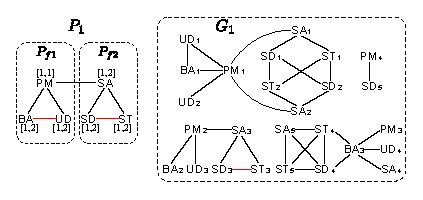
\includegraphics[scale=1.15]{./fig/motivation-example.eps}
\end{center}
\vspace{-3ex}
\caption{Motivation example}
\label{fig-motivation-example}
\vspace{-4ex}
\end{figure}

\eat{
A natural question is how to further capture the {\em structural and capacity constraints} in a unified model for team formation?
We essentially introduce a revision of graph pattern matching, an extension of graph simulation~\cite{infsimu95} and strong simulation~\cite{MaCFHW14}, for team formation to fill in this gap.
}%%%EAT

A natural question is how to further capture the {\em structural and capacity constraints} in a unified model for team formation?
We  introduce a revision of {\em graph pattern matching} for team formation to fill in this gap.
% 
Given a pattern graph $P$ and a data graph $G$, graph pattern matching is to find all subgraphs in $G$ that match $P$, and has been extensively studied~\cite{Ullmann76,infsimu95,FanLMTWW10,MaCFHW14,Guanfeng15,FanCount16}.  Essentially, we utilize patterns to captures the structural constraint, and revise the semantics of graph pattern matching for team formation. For instance, a desired team requirement can be specified by the pattern $P_1$ (ignore dashed edges) in Fig.~\ref{fig-motivation-example}, in which nodes represent the skill requirements,  edges specify the topology constraint, and the bounds on nodes are the capacity constraint.

%Especially, {\em strong simulation} introduces duality and locality into simulation, and shows a good balance between its computational complexity and its ability to preserve graph topology~\cite{MaCFHW14}.


Another issue it that team formation is accompanied with a highly dynamic situation. It typically needs many labor efforts to find the ideal teams, and is common for professionals to refine patterns  (requirements) multiple rounds~\cite{SajjadPG12,HabibiP15}. Further, real-life graphs are often big and constantly evolve over time~\cite{FanWW13-tods}. We illustrate this with an example.

\begin{example}
\label{exm-motivation-inc}
Consider $P_{1}$ and $G_{1}$ in Example~\ref{exm-motivation} again.
	
\sstab{(1)} % When the manager gets the match result, \ie the top-$k$ teams $P_{1}(G_{1})$ to $P_{1}$ in $G_{1}$,
One may find that $P_1$ is too restrictive to find any sensible match in  $G_{1}$.
Hence, she needs to refine the pattern by updating $P_1$ with $\Delta P_{1}$, \eg an edge
deletion $(\kw{SD},\kw{ST})^-$.
%We denote $P_{1}\oplus\Delta P_{1}$ the updated pattern.
%It is much better to derive $P_{1}\oplus\Delta P_{1}(G_{1})$ from $P_{1}(G_{1})$
%than a computation for $P_{1}\oplus\Delta P_{1}$ in $G_{1}$ from scratch.
%\looseness=-1
	
\sstab{(2)} It is also common that a data update $\Delta G_1$ comes on $G_1$, \eg an edge insertion $(\kw{SD_3},\kw{ST_3})^+$.
%Similar with (1), it is better to compute $P_{1}(G_{1}\oplus\Delta G_{1})$ from $P_{1}(G_{1})$ incrementally.
	
\sstab{(3)} Finally, it can be the case when pattern update $\Delta P_{1}$  and data update $\Delta G_{1}$ come simultaneously on $P_1$ and $G_1$.
%,  $P_{1}\oplus\Delta P_{1}(G_{1}\oplus\Delta G_{1})$ from $P_{1}(G_{1})$ incrementally
\end{example}

This motivates us to study the {\em dynamic top-k team formation} problem, to handle continuous
pattern and data updates, separately and simultaneously. It is known that incremental algorithms avoid re-computing from scratch by re-using previous results~\cite{inc-survey}. However, incremental algorithms of graph pattern matching for pattern updates has not been investigated, though there exist incremental algorithms of graph pattern matching for dealing with data updates~\cite{FanLMTWW10,FanWW13-tods,FanHT17}.
Further, it is also challenging for incremental algorithms to handle simultaneous pattern and data updates  in a unified way.



\eat{
often too costly to recompute top-$k$ teams from scratch in response to pattern and data updates.
These highlight the need for incremental algorithms to compute the updated top-$k$ teams.
As opposed to batch algorithms, incremental algorithms avoid re-computing from scratch by re-using previous results.
Traditional incremental algorithms for graph queries including graph pattern matching queries are proposed to compute changes in response to data updates, which has a lot of work~\cite{FanLMTWW10,FanWW13-tods,FanHT17}.
However, the study on incremental algorithms for graph pattern updates is in its vacancy.

Given a pattern graph $P$ and a data graph $G$, the graph pattern matching results $P(G)$ in $G$ for $P$ and changes $\Delta G$ to $G$ as input,
the traditional incremental matching problem is to compute changes $\Delta O$ to $P(G)$ such that $P(G\oplus\Delta G)$=$P(G)\oplus \Delta O$.
Here $\oplus$ denotes applying changes $\Delta S$ to $S$, when $S$ is data graph $G$ or query result $P(G)$.
It is to improve response time by reducing computations on big $G$ to small $\Delta G$ and $\Delta O$.

As a basis of \dynteamF, we also investigate the incremental problem for graph pattern matching on pattern updates.
The definition can be formulated along the same line with existing data incremental problems.
%different with data incremental algorithms that preserve some desirable properties that the recomputation can be {\em bounded}  by the changes in the input and output as the impact of data updates can be localized~\cite{Reps96, FanLMTWW10,FanWW13-tods,FanHT17},
However, devising pattern incremental algorithms is quite challenging as the impact of pattern updates is global,
due to the inherent hardness of the problem.
Despite of this, we devise an effective unified incremental approach for the \dynteamF\, problem.

 }%%%EAT






\looseness = -1

\stitle{Contributions}. To this end,  we introduce a graph pattern matching approach for (dynamic) top-$k$ team formation.


\stab (1) We propose {\em team simulation}, a revision of traditional graph pattern matching, for top-$k$ team formation (Section~\ref{sec-tsim}).
It extends existing methods by incorporating the structural and capacity constraints using pattern graphs .
To cope with the highly dynamic environment of team formation, we also formulate the dynamic top-$k$ team formation problem  (Section~\ref{sec-tsim}), for handling separate and simultaneous pattern and data updates.



\revise{
\stab (2) We develop a batch algorithm with two optimization techniques for computing top-$k$ teams via team simulation.}
We also study the satisfiability problem for pattern graphs, a new problem raised in the presence of capacity bounds for graph pattern matching (Section~\ref{sec-tsimAlg}).
We develop a unified approach to handling the need for both pattern and data updates.
We first prove that the dynamic top-$k$ team formation problem is unbounded even for single pattern or data updates, by extending the notion of incremental boundedness~\cite{Reps96}.
In light of this, we then propose an incremental strategy based on {\em pattern fragmentation} and {\em affected balls} to localize the effects of pattern and data updates (Sections~\ref{sec-dynamictopk}).
We finally develop a unified incremental algorithm for dealing with separate and simultaneous pattern and data updates,
with an optimization technique with the {\em early return} property for incremental top-$k$ algorithms, an analogy of the traditional early termination property (Sections~\ref{sec-IncAlg}).


\eat{%%%%%%%%%%%%%%%%move to section 3

As opposed to batch algorithms that recompute new match results from scratch,
incremental algorithms \cite{inc-survey} have been proposed to compute new match results,
by reusing and updating previous cached results according to the changes in input.
\looseness=-1

\begin{example}
\label{exm-motivation-inc}
Recall $P_{1}$ and $G_{1}$ in Fig.~\ref{fig-motivation-example} and continue.

\sstab{(1)} When the user gets the matched teams $P_{1}(G_{1})$ to $P_{1}$ in $G_{1}$, she may find $P_1$ is too restrictive to find possible teams.
Therefore, she enters pattern updates $\Delta P_1$ on $P_1$, composed of an edge deletion $(\kw{SD},\kw{ST})^-$.
We denote $P_{1}\oplus\Delta P_{1}$ the revised pattern.
It is much better to derive $P_{1}\oplus\Delta P_{1}(G_{1})$ from $P_{1}(G_{1})$
than a computation for $P_{1}\oplus\Delta P_{1}$ in $G_{1}$ from scratch.
\looseness=-1

\sstab{(2)} When data updates $\Delta G_1$ come on $G_1$, composed of an edge insertion $(\kw{SD_3},\kw{ST_3})^+$.
Similarly with (1), it is better to compute $P_{1}(G_{1}\oplus\Delta G_{1})$ from $P_{1}(G_{1})$ incrementally.

\sstab{(3)} Even better, when it comes to the case pattern $\Delta P_{1}$ and data updates $\Delta G_{1}$ come together, it is desirable to compute $P_{1}\oplus\Delta P_{1}(G_{1}\oplus\Delta G_{1})$ from $P_{1}(G_{1})$ incrementally.
\end{example}
}%%%%%%%%EAT



\eat{%%%EAT
%Hence, there is an urgent need to study the team formation problem in a dynamic setting.
These encourage us to propose the {\em dynamic top-$k$ team formation} problem (\dynteamF),
to handle separate and simultaneous pattern and data updates.
However, the problem is non-trivial.
There has been a bunch of work on data incremental algorithms on graphs~\cite{Reps96,FanWW13-tods},
but less work on handling pattern updates is known, and furthermore less work on handling both data and pattern updates is known. The challenges comes from three aspects:
(a) the nature of pattern updates, pattern updates have significant impacts on the match results.
A unit update is likely to result in the entire change in match results, such that all previous match results need to be re-computed, which is actually a costly batch computation;
(b) the demand to design light weight and effective auxiliary data structures for the dynamic team formation problem, concerning the space consumption and the efficiency;
and (c) the requirement to design a {\em one-method-fits-two} model, to support pattern and data updates simultaneously and separately.

To solve the {\em top-$k$ team formation} problem and the {\em dynamic top-$k$ team formation} problem, several fundamental problems call for a full treatment.
(1) How to extend graph pattern matching for top-$k$ team formation to retain the properties in existing methods, and pursue more practical usage,
%such as combine capacity bound and structural constraints on matched results,
without sacrificing the efficiency?
(2) How to efficiently support pattern updates for, \eg user query adjustments on patterns, by reusing previous cached results as much as possible?
(3) How to handle data updates to meet the practical requirements?
(4) How to design a unified incremental model to handle both pattern and data updates efficiently in a simultaneous manner?
}%%%EAT

\eat{
\stitle{Contributions}. To this end,  we introduce a graph pattern matching approach for (dynamic) team formation.

\stab (1) We propose {\em team simulation} for top-$k$ team formation, a revision of traditional graph pattern matching,
which extends existing methods {\em strong simulation} for team formation by incorporating the structural and capacity constraints using pattern graphs  (Section~\ref{sec-tsim}).
We also study the satisfiability problem for pattern graphs, a new problem raised in the presence of capacity bounds for graph pattern matching.
We finally develop an efficient cubic batch algorithm with two optimization techniques, \ie density based filtering and pattern minimization, for computing top-$k$ teams via team simulation.

\stab (2) We formulate the dynamic top-$k$ team formation problem, and develop a unified approach to handling the need for both pattern and data updates (Sections~\ref{sec-dynamictopk} \& \ref{sec-IncAlg}).
We first prove that the  problem is unbounded even for single pattern or data updates, by extending the notion of incremental boundedness~\cite{Reps96}.
In light of this, we then propose an incremental strategy based on {\em pattern fragmentation} and {\em affected balls} to localize the effects of pattern and data updates. We finally develop a unified incremental algorithm for dealing with continuous pattern and data updates, separately and simultaneously,
with an optimization technique with the {\em early return} property for incremental top-$k$ algorithms, an analogy of the traditional early termination property.
}%%%EAT

\eat{%%%EAT
\stab (3) Using real-life and synthetic graphs, we experimentally verify the effectiveness and efficiency of the static and dynamic top-$k$ graph pattern matching model and optimization techniques, for separate and simultaneous pattern and data updates, for solving \teamF\,and \dynteamF\,problems.
{\bf Add details}
}%%%EAT

\stab (3) Using real-life data (\citationd) and synthetic data (\synthetic), we demonstrate the effectiveness and efficiency of our graph pattern matching approach for (dynamic) team formation (Section~\ref{sec-expt}).
We find that (a) our method is able to identify more sensible teams than existing team formation methods \wrt \eat{three} practical measurements,
and (b) our incremental algorithm outperforms our batch algorithm, even when changes reach 36\% for pattern updates, 34\% for data updates and (25\%, 22\%) for simultaneous pattern and data updates, and when 29\% for continuous pattern updates, 26\% for continuous data updates and (20\%, 18\%) for continuous simultaneous pattern and data updates, respectively.


To our knowledge, this work is among the first to study simultaneous pattern and data incremental computations, no previous work has studied pattern updates for incremental pattern matching~\cite{FanHT17,FanWW13-tods}, not to mention continuous and simultaneous pattern and data updates.  This is  the most general dynamic setting for incremental computations.

All detailed proofs are available  in the full version~\cite{fullvldb18}.

\stitle{Related work}. Previous work can be classified as follows.

%\etitle{Graph pattern matching}.

 Graph simulation \cite{infsimu95} and its extensions have been introduced for graph pattern matching~\cite{FanLMTWW10,MaCFHW14,Guanfeng15,FanCount16}, in which {\em strong simulation} introduces duality and locality into simulation~\cite{MaCFHW14}, and shows a good balance between its computational complexity and its ability to preserve graph topology. Furthermore, \cite{FanCount16} already adopts capacity bounds on the edges of pattern graphs via subgraph isomorphism, and \cite{FanWWXin13} uses graph pattern matching to find single experts, instead of a team of experts. In this study, team simulation is proposed for team formation as an extension of graph simulation and strong simulation on undirected graphs with capacity constraints on the nodes of pattern graphs.


%\etitle{Team formation}.

There has been a host of work on team formation by minimizing the communication cost of team members, based on the diameter, density, minimum spanning tree, Steiner tree, and sum of pairwise member distances among others \cite{Lappas09,Kargar11,ArisLuca12,GajewarS12,realTeamForm13,SamikKVM12,LiTongCao15}, which are essentially  a specialized class of keyword search on graphs~\cite{Aggarwal10}. Similar to~\cite{Kargar11}, we are to find top-$k$ teams. However, \cite{Kargar11} adopted Lawler's procedure \cite{Lawler1972}, and is inappropriate for large graphs. We also adopt {\em density}  as the communication cost, which shows a better performance~\cite{GajewarS12}, and further require that all team members are {\em close to each other} (located in the same balls), along the same line with~\cite{Lappas09,Kargar11,ArisLuca12,SamikKVM12}.
\revise{Except for simply minimizing the communication cost among team members,
\cite{HuangLv16,Kargar11} consider minimizing the cost among team members and team leaders.}
Different from these work, we introduce {\em structural constraints}, in terms of graph pattern matching~\cite{FanLMTWW10,MaCFHW14}, into team formation, while retaining the capacity bounds on specific team members like~\cite{realTeamForm13,GajewarS12}.



%\etitle{Incremental computations}.

Incremental algorithms (see \cite{inc-survey,FanHT17} for a survey) have proven usefulness in a variety of applications,
and have been studied for graph pattern matching~\cite{FanLMTWW10,FanWW13-tods} and team formation \cite{ArisLuca12} as well.
However, \cite{inc-survey,FanHT17,FanLMTWW10,FanWW13-tods} only consider data updates,
and \cite{ArisLuca12} only considers continuous coming new tasks. In this work, we  deal with both pattern and data updates for team formation, and support both insertions and deletions. To our knowledge, this is the first study on pattern updates, and is the most general and practical dynamic setting considered so far.

{Query reformulation (\aka query rewriting /modification) is to generate alternative queries that may produce better answers,
and has been studied for structured queries~\cite{MottinEmpty13}, keyword queries~\cite{YaoQReform12} and graph queries~\cite{MottinGReform15}.
However, different from our study of handling pattern updates, the focus of query reformulation is not on incremental computations.

%\etitle{Top-k queries}.

Although top-$k$ queries (see~\cite{IlyasBS08} for a survey) have been studied for both graph pattern matching and team formation~\cite{Kargar11},
they have never been studied for both team formation and graph pattern matching  in a dynamic setting.


\eat{
\etitle{Query reformulation}. \textcolor{blue}{Query reformulation (\aka query rewriting/modification) is to provide users with a set of specializations of the original query that may better capture their search intent.
It has been studied for structured queries~\cite{MottinEmpty13}, keyword queries~\cite{YaoQReform12} and graph queries~\cite{MottinGReform15}.
However, they all aim at automatically providing alternative queries (\eg supergraphs~\cite{MottinGReform15}) to users,
while care less about answering the changed queries.
In this work, we focus on handling query modification from users and how to quickly return the answers based on previous answers.}
}

\eat{%%%EAT
To retain the properties in existing methods, and pursue more practical usage, we incorporate the capacity bounds, density measure and locality into graph simulation as the matching semantics.

When a user inputs a pattern graph into a system with a data graph already stored in it, and gets the match result, sometimes he or she may find that the query is not appropriate in some sense after an analysis on the result. Then the user probably makes some small adjustments on the pattern graph. However, it is expensive to recompute the matches from scratch via batch algorithm due to the slight change in pattern graph, and this comes the convenience for executing incremental graph matching, which just computes changes in the match result corresponding to the updates in pattern graph.
}%%%EAT

\newcommand{\grouprec}{\kw{batch}}
\newcommand{\optgrouprec}{\kw{batch}}
%\newcommand{\grouprecopt}{\kw{kTeamFormOpt}}
\newcommand{\minp}{\kw{minP}}
\newcommand{\rgraphsim}{\kw{undirgSim}}
\newcommand{\incsim}{\kw{incSim}}


\section{Dynamic Team Formation}
\label{sec-tsim}


We first propose {\em team simulation}, a revision of traditional graph pattern matching.
We then formally introduce the {\em top-$k$ team formation} problem via team simulation.
We finally present the {\em dynamic top-$k$ team formation} problem.

\eat{
In this section, we first present basic notations of graphs, and then propose team simulation, an extension of traditional graph pattern matching.
We finally formally introduce the top-$k$ team formation problem via team simulation, and propose a cubic algorithm with two optimization techniques.

\subsection{Data Graphs and Pattern Graphs}
\label{subsec-graphdefs}


\stitle{Data graphs}.
A {\em data graph} is a labeled undirected graph $G(V, E, l)$, where
(1) $V$ is a finite set of nodes;
(2) $E \subseteq V \times V$, in which $(u, u')$ or $(u', u)$ $\in E$ denotes an undirected edge between nodes $u$ and $u'$; and
(3) $l$ is a total labeling function that maps each node in $V$ to a set of labels.

%; and(4) $w$ is a total weight function that maps each edge in $E$ to a positive rational number.

Intuitively, the node labels carry the content of the node, \eg skills, keywords, blogs, rating~\cite{AmerYahiaBB07}.
The edges specify the affinity or collaborative compatibility among nodes~\cite{GajewarS12}.

\stitle{Pattern graphs}.
A {\em pattern graph} (or simply pattern) is an undirected graph $P(V_P$, $E_P$, $l_P$, $f_P)$, in which
(1) $V_P$ and $E_P$ are the set of nodes and the set of edges, respectively;
(2) $l_P$ is a total labeling function that maps each node in $V_P$ to a single label; and
(3) $f_P$ is a total capacity function such that for each node $u\in V_P$, $f_P(u)$ is a closed interval $[x, y]$, where $x\le y$ are non-negative integers.

Intuitively, $f_P(u)$ specifies a range bound for node $u$,
indicating the required quantity for the matched nodes in data graphs.
Note that for traditional graph patterns~\cite{Galla06, b-matching,FanLMTWW10,FanCount16}, bounds are typically carried on edges, not on nodes.
\looseness=-1


\begin{example}
\label{exm-pattern}
Consider pattern graph $P_1$ and data graph $G_1$ in Fig.~\ref{exm-motivation}. Observe that there is a capacity bound on each node in $P_1$.
For example, capacity bound [1,2] on node \kw{SD} in $P_1$ indicates in the match result,
there should be at least one and at most two nodes matched with \kw{SD}.
\end{example}


\stitle{Remarks}. We assume \kwlog~that pattern graphs are connected, as a common practice.
We also simply denote data graphs $G(V, E, l$) as  $G(V, E)$ and pattern graphs $P(V_P$, $E_P$, $l_P$, $f_P)$ as $P(V_P$, $E_P)$, respectively.
Furthermore, the size $|G|$ of data graphs $G$ (resp. $|P|$ of pattern graphs $P$) is the total number of nodes and edges in $G$ (resp. $P$).
}%%%EAT

\eat{%%%%%%%%%%%%%%%%
We shall use the following notation
	
\etitle{Subgraphs}.
Graph $H(V_s, E_s,  l_{H})$ is a {\em subgraph} of data graph $G(V, E, l)$, denoted as $G[V_s, E_s]$, if
(1) for each node $u\in V_s$, $u\in V$ and $l_{H}(u) = l(u)$, and
(2) for each edge $e\in E_s$, $e\in E$. % and $w_{H}(e) = w(e)$.
That is, subgraph $G[V_s, E_s]$ only contains a subset of nodes and a subset of edges of graph $G$.

We also denote subgraph $G[V_s, E_s]$ as subgraph $G[V_s]$, if $E_{s}$ is exactly


Similarly, we can define {\em subgraphs for pattern graphs}, which further requires the preservation of the node capacity.

\etitle{Induced subgraphs}. An {\em induced subgraph} $G_{s}(V_{s}, E_{s})$ is composed of vertices $V_{s}$ who is a subset of the vertices $V$ of graph $G(V, E)$, and together with the edge set $E_{s}$ whose endpoints are both in $V_{s}$ in $G(V, E)$.


\etitle{Subpatterns}.
Pattern $Q(V_s, E_s,  l_{q}, f_{q})$ is a {\em subpattern} of pattern $P(V_p$, $E_p$, $l_p$, $f_p)$, denoted as $P[V_s, E_s]$, if
(1) for each node $u\in V_s$, $u\in V$, $l_{q}(u) = l_p(u)$ and $f_{q}(u) = f_p(u)$, and
(2) for each edge $e\in E_s$, $e\in E$. % and $w_{H}(e) = w(e)$.
That is, subpattern $G[V_s, E_s]$ only contains a subset of nodes and a subset of edges of pattern $P$.}

% \etitle{Connected components}.
% A {\em connected component} of a graph is a subgraph in which any two nodes are connected to each other by undirected paths,
% and which is only connected to the nodes of itself, \ie a connected component is maximal.
% A graph that is itself connected has exactly one connected component, which is the entire graph.

\eat{%%%%%%%%%%%
\etitle{Neighbors}. We say that node $u'$ is a {\em neighbor} of node $u$ if there is an edge between $u$ and $u'$ in a data or pattern graph.

\etitle{Paths}.
A {\em simple path} (or simply a {\em path}) $\rho$ is a sequence of nodes $v_1/\ldots/v_n$ with no repeated nodes, and, moreover, for each $i\in[1, n-1]$, $(v_i$, $v_{i+1})$ is an edge in $G$. The {\em length} of a path $\rho$ is the number of edges in $\rho$.

A graph is {\em connected} if for each pair of nodes, there exists a  path connecting them.

\etitle{Distances}. Given two nodes $v$ and $v'$ in a graph $G$, the {\em  distance} from $v$ to $v'$,
denoted by $\dist(v,v')$, is  the shortest length of all {\em paths}
from $v$ to $v'$ in $G$.
}


\eat{%%%%%%%%%%
\etitle{Diameter}. The {\em diameter} of a connected graph $G$,  denoted by $\diameter{G}$, is the longest shortest distance of all pairs of nodes in $G$, \ie $\diameter{G}$ = $\kw{max}(\kw{dis}(v,v'))$ for all nodes $v,v'$ in $G$.
}%%%%%%%%%%%%%%


\eat{
\etitle{Distances}. The {\em length} of a path $\rho$ is
the sum of the weights of its constituent edges, \ie $\sum_{i=1}^{n-1} w(v_i, v_{i+1})$.

Given two nodes $v, v'$ in a graph $G$, the {\em distance} from $v$ to $v'$,
denoted by $\dist(v,v')$, is the length of the shortest {\em path}
from $v$ to $v'$ in $G$.
}

%\vspace{-4ex}
\subsection{Team Formation}
\label{subsec-extsim}

We first extend pattern graphs of traditional graph pattern matching to carry capacity requirements,
and then define team simulation on undirected graphs.
%We then redefine strong simulation on directed graphs, originally defined on directed graphs~\cite{MaCFHW14}.}

We start with basic notations.

\stitle{Data graphs.} A {\em data graph} is a labeled undirected graph $G(V$, $E$, $l)$, where $V$ and $E$ are the sets of nodes and edges, respectively; and $l$ is a total labeling function that maps each node in $V$ to a set of labels.

\stitle{Pattern graphs}.
A {\em pattern graph} (or simply pattern) is an undirected graph $P(V_P$, $E_P$, $l_P$, $f_P)$, in which
(1) $V_P$ and $E_P$ are the set of nodes and the set of edges, respectively;
(2) $l_P$ is a total labeling function that maps each node in $V_P$ to a single label; and
(3) $f_P$ is a total capacity function such that for each node $u\in V_P$, $f_P(u)$ is a closed interval $[x, y]$, where $x\le y$ are non-negative integers.

Intuitively, $f_P(u)$ specifies a range bound for node $u$,
indicating the required quantity for the matched nodes in data graphs.
Note that for traditional patterns~\cite{Galla06, b-matching,FanLMTWW10,FanCount16}, bounds are typically carried on edges, not on nodes.

We also also denote data and pattern graphs as $G(V$, $E)$ and $P(V_{P}$, $E_{P})$ respectively. The size of $G$ (resp. $P$), denoted by $|G|$ (resp. $|P|$), is defined to be the total number of nodes and edges in $G$ (resp. $P$).

%We define $r$-simulation by extending graph simulation~\cite{infsimu95,FanLMTWW10,MaCFHW14} on undirected graphs  and introducing capacity constraints.

\eat{As strong simulation is an extension of graph simulation, which is also defined on directed graphs~\cite{infsimu95,FanLMTWW10},
We now redefine graph simulation on undirected graphs. Consider a pattern graph $P(V_P$, $E_P)$ and a data graph $G(V$, $E)$.
}%%%EAT

We now redefine graph simulation on undirected graphs, which is originally defined on directed graphs~\cite{infsimu95,FanLMTWW10}. Consider pattern graph $P(V_P$, $E_P)$ and data graph $G(V$, $E)$.


\stitle{Graph simulation}. Data graph $G$ {\em matches} pattern graph $P$ via
graph simulation, denoted by $P \eps G$, if there exists a binary {\em match relation} $\Reps \subseteq V_P \times V$ in $G$ for $P$ such that

\vspace{0.5ex}
\ni
(1) for each $(u, v) \in \Reps$, the label of $u$ matches one label in the label set of $v$, \ie $l_{P}(u) \in l(v)$; and

\vspace{0.5ex}
\ni
(2) for each node  $u\in V_P$, there exists $v\in V$ such that
(a) $(u, v) \in \Reps$, and
(b) for each adjacent node $u'$ of $u$ in $P$, there exists a adjacent node $v'$ of $v$
in $G$ such that $(u',v') \in \Reps$.

For any $G$ that matches $P$, there exists a {\em unique maximum} match relation via graph simulation~\cite{infsimu95}.

We then introduce the notions of balls and match graphs.

%While there may be multiple match relations in a graph $G$ for a pattern graph $P$,
%there exists a unique {\em maximum} match relation $\Reps_m$ in $G$ for $P$ such that for any match relation $R$ in $G$ for $P$, $\Reps \subseteq \Reps_m$,

\eat{%%%EAT
Intuitively, graph simulation preserves the label match and
neighborhood relationships between pattern graphs and the matched data graphs~\cite{FanLMTWW10,MaCFHW14}.

Following from \cite{FanLMTWW10,MaCFHW14}, the revised graph simulation above is well-defined, as shown below.
%Following from \cite{FanLMTWW10,MaCFHW14}, it is easy to know that the graph simulation revised above has the following.

\begin{prop}
\label{prop-sim-maximum-match}
For any data graph $G$ and pattern graph $P$  such that $P\eps G$, via graph simulation, there is a unique maximum match relation in $G$ for $P$.
\end{prop}
}%%%EAT


\etitle{Balls}. For a node $v$ in data graph $G$ and a non-negative integer $r$,
the {\em ball} with {\em center} $v$ and {\em radius} $r$  is a subgraph of $G$,
denoted by $\ball{[v, r]}$, such that (1) all nodes $v'$ are in $\ball{[v, r]}$, if
the number of hops between $v'$ and $v$, $\hop(v', v)$, is no more than $r$, and (2) it has exactly the edges
appearing in $G$ over the same node set.

\eat{%%EAT
Intuitively, a ball is a connected graph such that all node pairs have bounded hops.
Indeed, as observed in~\cite{Buchan2004}, when social distance increases, the
closeness of relationships decreases and the  relationships may become
irrelevant. Hence it often suffices in practice to consider only those
matches of a pattern graph that fall in a small ball.
}%%%EAT

\etitle{Match graphs}. The {\em match} graph $\wrt$ a binary relation $\Reps\subseteq V_P\times V$ is a subgraph $G_s$ of data graph $G$, in which
(1)  a node $v\in V_s$ if and only if it is in $\Reps$, and
(2) it has exactly the edges
appearing in $G$ over the same node set.

Intuitively, the match graph $G_s$ $\wrt$ $\Reps$ is the induced subgraph of
$G$ such that its nodes play a role in $\Reps$.


\eat{%%%%EAT
\stitle{Induced match graphs}. Consider a binary relation $\Reps\subseteq V_q\times V$.
The {\em induced match} graph $\wrt$ $\Reps$ is a induced subgraph $G[V_s, E_s]$ of $G$, in which
(1) a node $v\in V_s$ if and only if it is in $\Reps$, and
(2) an edge $(v,v')\in E_s$ if and only if $v$ and $v'$ are in $\Reps$.
%
Intuitively, the induced match graph $G[V_s, E_s]$ $\wrt$ $\Reps$ is the induced subgraph of $G$ such that each of its nodes plays a role in $\Reps$, together with the adjacent edges in $G$.
}%%%%%%%%%EAT

We are now ready to define team simulation, by extending graph simulation to incorporate the locality constraints enforced by balls, and the capacity bounds carried by patterns.
\looseness=-1

%\vspace{-1ex}
\stitle{Team simulation}. Data graph $G$ {\em matches} pattern $P$  via
team simulation \wrt a radius $r$, denoted by $P \eeps G$, if
there exists a {\em ball} $\ball{[v, t]}$ ($t \in [1,r]$, $t \in Z$) in $G$, such that

\vspace{0.5ex}
\ni(1) $P\eps \ball{[v, t]}$, with the maximum match relation $\Reps$ and the match graph $G_s$ $\wrt$ $\Reps$; and

\vspace{0.5ex}
\ni(2) for each node $u$ in $P$, the number of nodes $v$ in $G_s$  with $(u, v)\in \Reps$ falls into $f_P(u)$.

\vspace{0.5ex}
We refer to  $G_s$ as a {\em perfect} subgraph of $G$ \wrt $P$.


Intuitively, (1) pattern graphs $P$ capture the structural and capacity constraints, and (2) a perfect subgraph $G_s$ of pattern $P$ corresponds to a desired team, which is required to satisfy the following conditions:
(a) $G_s$ itself is located in a ball $\ball{[v, t]}$  where $t \in [1,r]$ as a match graph; and
(b) $G_s$ satisfies the capacity constraints carried over pattern $P$.



\begin{example}
\label{exm-rsimulation}
Consider pattern $P_1$ and data graph $G_1$ in Fig.~\ref{exm-motivation}, and  team simulation with $r=2$ is adopted.

One can easily verify that $P_1$ matches $G_1$  via team simulation, \ie $P_1 \eeps G_1$,
as (a) there is a perfect subgraph in in ball
$\ball{[\kw{PM_1}, 2]}$, \ie the connected component of $G_1$ containing $\kw{PM_{1}}$, which maps \kw{PM}, \kw{BA}, \kw{UD}, \kw{SA}, \kw{SD} and \kw{ST} in $P_1$ to \kw{PM_1}, \kw{BA_1}, \{\kw{UD_1}, \kw{UD_2}\}, \{\kw{SA_1}, \kw{SA_2}\}, \{\kw{SD_1}, \kw{SD_2}\} and \{\kw{ST_1}, \kw{ST_2}\}, respectively, and, moreover, (b) the capacity bounds on all pattern nodes are satisfied.
\end{example}

\eat{%%%170720
\stitle{Remarks}.
(1) Graph simulation is a special case of team simulation on undirected graphs,
when the capacity on each pattern node is $[1, +\infty]$, and $r$ is no less than the diameter of data graphs.
%
(2) Further, strong simulation is also a special case of team simulation on undirected graphs,  when the capacity on each pattern node is $[1, +\infty]$,
$r$ is equal to the diameter of pattern graphs, and match graphs only involve with those edges matching edges in pattern graphs.
}%%%EAT170720

\stitle{Remarks}.
(1) Team simulation differs from graph simulation~\cite{infsimu95} and strong simulation~\cite{MaCFHW14} in the existence of capacity bounds on pattern graphs and its ability to capture matches on undirected graphs.

\sstab(2) Different from strong simulation with balls having a fixed radius (\ie the diameter of a pattern), team simulation adopts a more natural setting that the radius of the balls is flexible, and is only less than a user specified upper bound.

%(2) Graph simulation (resp. strong simulation) is a special case of team simulation on undirected graphs when the capacity on each pattern node is $[1, +\infty]$, and $r$ is no less than (resp. equal to) the diameter of data graphs (resp. pattern graphs).





\eat{%%%EAT
\stitle{Remarks}.
(1) Graph simulation is a special case of (1) team simulation for undirected graphs,
when the capacity on each pattern node is $[1, +\infty]$ and $r$ is no less than the diameter of data graphs.
%
(2) Graph simulation~\cite{FanLMTWW10} and dual simulation~\cite{MaCFHW14} are equal on undirected graphs.
Hence, many good properties of dual simulation naturally carry over to graph simulation on undirected graphs.
%
(3) {\bf The difference of matched graphs between strong simulation and T-simulation.}
}%%%EAT

%and also a special case of (2) subgraph isomorphism, when the labels on pattern nodes are different from each other and the capacity on each pattern node is $[1, 1]$.

%(1) Graph simulation and its extensions were originally proposed on directed graphs.
%They were introduced for social networks analysis~\cite{BrynielssonHKMS10}, and for graph pattern matching~\cite{FanLMTWW10,FanLMTW11} due to its low \PTIME
%computational complexity~\cite{infsimu95}.


\eat{%%%%%%%%

When given a pattern graph, we first make a examination on it ensuring that there exist data graphs in which we can find matches using the pattern graph. If the answer is true, we can execute the following computing work. Otherwise, we require the user to retype in another pattern graph.
}


\eat{%%%170720
\begin{figure}[tb!]
%\vspace{-1ex}
\begin{center}
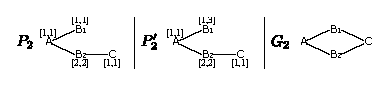
\includegraphics[scale=1.28]{./fig/consistency_motivation.eps}
\end{center}
\vspace{-3ex}
\caption{Pattern graphs}
\vspace{-4ex}
\label{fig-consistency-example}
\end{figure}

\stitle{Pattern satisfiability}.
We say that a pattern $P$ is {\em satisfiable} iff there exists a data graph $G$ such that $P \eeps G$.



Different from graph simulation \cite{infsimu95} and its extensions \cite{FanLMTWW10,MaCFHW14},
pattern graphs may be unsatisfiable for team simulation, due to the presence of capacity constraints enforced on patterns. We illustrate this with an example below.
%\looseness=-1

\begin{example}
\label{exm-consistency}
\ni(1)  Consider pattern $P_2$ in Fig.~\ref{fig-consistency-example}.
One can verify that there exist no data graphs $G$ such that $P_2 \eeps G$ because (a) for any nodes $u$ in $G$, if $u$ matches with the node labeled with $B_2$, then it must match with the node labeled with $B_1$, and, hence, (b) the capacity upper bound on $B_1$ should not be less than the lower bound on $B_2$.


\sstab(2) Pattern $P_1$ in Fig.~\ref{exm-motivation} is satisfiable as $P_1 \eeps G_1$.
\end{example}


The good news is that checking the satisfiability of pattern graphs can be done in low polynomial time.

\begin{prop}
\label{prop-pattern-consistency}
The satisfiability of patterns $P$ can be checked in $O(|P|^2)$ time.
\end{prop}

\proofS By treating $P$ as both data and pattern graphs, compute the maximum match relation $M$ in $P$ for $P$, via graph simulation.
Indeed, pattern $P$ is satisfiable iff for each $(u, v)\in M$ with the capacity bounds $[x_u, y_u]$ on $u$ and $[x_v, y_v]$ on $v$, respectively, $x_v \leq y_u$ holds. Observe that the size of $M$ is bounded by $|P|^2$.
\eop

Pattern graphs are typically small, and we only consider  satisfiable patterns in the sequel, by Proposition~\ref{prop-pattern-consistency}.
}

\subsection{Top-k Team Formation}
\label{subsec-teamF}

 Given pattern $P$, data graph $G$, and two positive integers $r$ and $k$, the {\em top-$k$ team formation} problem, denoted as \teamF{(P, G, k)},
is to find a list $L_{k}$ of $k$ perfect subgraphs (\ie teams) with the top-$k$ largest density in $G$ for $P$, via team simulation.
\looseness=-1

Here the {\em density}\, $\density{G}$ of graph $G(V, E)$ is $|E|/|V|$, where $|E|$ and $|V|$ are the number of edges and the number of nodes respectively, as commonly used in data mining applications~\cite{maximumDenseSubgraph,EVMK12}.
Intuitively, the larger $\density{G}$ is, the more collaborative a team is.
In this way, not only the two objective functions of existing team formation methods are preserved,
\ie the locality retained by balls and the density function in selecting top-$k$ results,
but also the relationships among members and the capacity constraint on patterns.


\begin{example}
\label{exa-teamF}
Consider $P_1, G_1$ in Fig.~\ref{exm-motivation} and $r=2$.
We simply set $k=1$, as most existing solutions for \teamF{} only compute the best team \cite{Lappas09,ArisLuca12,GajewarS12,realTeamForm13,SamikKVM12}.

One may want to look for candidate teams with existing methods, satisfying the search requirement in Example \ref{exm-motivation}:
\ni(1) by minimizing the {\em team diameter} \cite{Lappas09},
which returns the team with $\{\kw{BA_3}$, \kw{PM_3}, \kw{UD_4}, \kw{SA_4}, \kw{SD_4}, $\kw{ST_4}\}$,

\ni(2) by minimizing the {\em sum of all-pair distances} of teams \cite{Kargar11},
which returns exactly the same team as (1) in this case, or

\ni(3) by maximizing the {\em team density} \cite{GajewarS12}, which returns the team with all the nodes in the two connected components in $G_1$ with \kw{PM_1} and \kw{BA_3}, except \kw{UD_2}, \kw{PM_3}, \kw{UD_4}, \kw{SA_4}.

One may already notice that these teams only satisfy the skill requirement, \ie condition (i) in Example \ref{exm-motivation}, and cannot guarantee  the specific collaboration relationships among team members.
Indeed, the team found in (1) and (2) is connected by \kw{BA_3} only, and the team found in (3) has loose collaborations among its members.
That is, existing methods are not appropriate for identifying the the desired teams.

When team simulation is adopted, it returns the perfect subgraph in Example \ref{exm-rsimulation} with its density = 1.4,
satisfying both conditions (i) and (ii), much better than those teams found by the above existing methods.
\end{example}

\eat{%%%EAT
\sstab
(a) Algorithm \mindia~\cite{Lappas09} is to find a team with the {\em minimum diameter}, and returns $\{\kw{BA_3}$, \kw{PM_3}, \kw{UD_4}, \kw{SA_4}, \kw{SD_4}, $\kw{ST_4}\}$.

\sstab
(b) Algorithm \minsumdis~\cite{Kargar11} aims at minimizing the sum of all-pair distances, which is an extension of \mindia, and it returns exactly the same team as \mindia in this case.

\sstab
(c) Algorithm \denalk~\cite{GajewarS12} is to find a team with the {\em largest density}, and
returns the subgraph consisting of the two connected components of $G_1$ containing \kw{PM_1} and \kw{BA_3} respectively (excluding \kw{UD_1},\kw{PM_3},\kw{UD_4},\kw{SA_4}), whose density is 1.5.
%Indeed, larger density always results in a larger quantity.

\sstab
(d) Our team simulation returns the perfect subgraph in Example \ref{exm-rsimulation} with its density = 1.4 as the best team.

One can see that only team simulation captures the topology, cardinality and collaboration requirements of teams.
}%%%EAT



\eat{%%%EAT170720
\begin{figure}[t!]
%\vspace{-2ex}
\begin{center}
{\small
\myhrule
\vspace{-3ex}
\mat{0ex}{
\sstab {\sl Input:\/} $G(V$, $E)$, $P(V_P$, $E_P)$, and positive integers $k, r$.\\
{\sl Output:\/} The list $L_{k}$ of top-$k$ teams\\
\sstab \bcc \hspace{1ex} \= $L_{k} := \emptyset$;\\
\icc \> \For each ball $\ball{[v,r]}$ in $G$ \Do\\
\icc \>\hspace{2ex}\= $G_s$ := \rgraphsim$(P, \ball{[v,r]})$;\\
\icc \>\> \If $\density{G_s}>$ the density of the $k$-th result in $L_{k}$ \Then\\
%\icc \>\> \If $\density{G_s}>$ the density of $kth$ result in $L_{k}$ and there exists\\
%     \>\>\hspace{0.5ex}   no $G'_s$ in $L_{k}$ that is same with $G_{s}$ \Then\\
\icc \>\>\hspace{2ex}\= remove the $k$-th result in $L_{k}$ and insert $G_s$ into $L_{k}$;\\
\icc \> \Return $L_{k}$.
}

\vspace{-4ex} \myhrule
}
\end{center}
\vspace{-3ex}
\caption{Algorithm \grouprec} \label{alg-grouprec}
\vspace{-4ex}
\end{figure}

We now present an algorithm for \teamF{} via team simulation.


\stitle{Algorithm for Top-k Team Formation.} Given $P$, $G$, and two integers $r$ and $k$, an algorithm, referred to as \grouprec, is shown in Fig.~\ref{alg-grouprec}.
\grouprec is to find the set of perfect subgraphs $G_s$ by inspecting those balls $\ball{[v, r]}$ centered at each node $v$ of $G$, and returns the top-$k$ densest ones.
It computes the perfect subgraph $G_s$ of $P$ in the ball $\ball{[v,r]}$ via team simulation by invoking \rgraphsim(lines 2-3).
Procedure \rgraphsim is deferred to the appendix, which is an adaption from graph simulation~\cite{infsimu95,FanLMTWW10},
by extending from directed to undirected graphs,  incorporating the capacity constraint check, and only maintaining the capacity bounds satisfied perfect subgraphs.
In the process, \grouprec maintains the top-$k$ non-repeated perfect subgraphs with current top-$k$ largest density (lines 4-5), and returns them when all balls are processed (line 6).


\begin{example}
\label{exa-alg-batch} Consider $r=2$ and $k=2$.

\sstab(1) For $P_1$ and $G_1$ (ignore dashed edges) in Fig.~\ref{fig-motivation-example},
 \grouprec returns the team found in Example~\ref{exm-rsimulation} as its only answer.

\sstab(2) For $P_1$ and $G_1$ (with dashed edges), \grouprec returns the team in (1) as the best,
and the connected component containing \kw{PM_2} with its density = 1 as the second best.
\end{example}


\stitle{Correctness \& complexity analyses}. The correctness of algorithm \grouprec is assured by the following.
(1) There is a unique perfect subgraph in each ball of $G$.
(2) The correctness of \rgraphsim can be verified along the same lines as for simulation~\cite{infsimu95}.
(3) The list $L_{k}$ always maintains the current top-$k$ teams with largest density.
It takes $O(|V||P||G|)$ time to compute team simulation for all balls,
and $O(|V|\cdot(|V_{G_s}|^2+|G_s|))$ time to maintain the top-$k$ teams.
Thus \grouprec is in $O(|V|\cdot(|P||G|+|V_{G_s}|^2))$ time.
}%%%EAT170720


\subsection{Dynamic Top-k Team Formation}
\label{subsec-dynteamF}

We now introduce dynamic top-$k$ team formation.
%For convenience, the notations used are summarized in Table~\ref{tab-notation}.

\stitle{Pattern updates ($\Delta P$)}. There are five types of pattern updates:
%
(1) {\em edge insertions} connecting nodes in $P$,
%
(2) {\em edge deletions} disconnecting nodes in $P$,
%
(3) {\em node insertions} attaching new nodes to $P$,
%
(4) {\em node deletions} removing nodes from $P$, and
%
(5) {\em capacity changes} adjusting the node capacities in $P$,
%
while $P$  remains connected in all cases.


\stitle{Data updates ($\Delta G$)}. There are four types of data updates,
defined along the same lines as the first four types of pattern updates.
Further, different from pattern updates, there is no need to keep $G$ connected for data updates.


\stitle{Dynamic top-$k$ team formation}. Given pattern $P$, data graph $G$, positive integers $r$ and $k$, the list $L_{k}(P,G)$ of top-$k$ perfect subgraphs for $P$ in $G$,
a set of pattern updates $\Delta P$ and a set of data updates $\Delta G$,
the {\em dynamic top-k team formation} problem, denoted by \dynteamF{(P, G, k, L_{k}, \Delta P, \Delta G)},
is to find a list of $k$ perfect subgraphs with the top-$k$ largest density for $P\oplus\Delta P$ in $G\oplus\Delta G$, via team simulation.


Here $\oplus$ denotes applying changes $\Delta P$ to $P$ and $\Delta G$ to $G$, and
 $P\oplus\Delta P$ and $G\oplus\Delta G$ denote the updated pattern and data graphs.
 It is worth mentioning that \dynteamF{} covers a broad range of dynamic situations,
\ie handling continuous separate and simultaneous pattern and data updates.

\eat{
\begin{example}
\label{exm-dyn-team}
Recall $P_1$, $G_1$, $\Delta P_1$ and $\Delta G_1$ in Example \ref{exm-motivation-inc} (3), and set $r=2$ and $k=2$.
When get the top-$2$ teams for $P_1$ in $G_1$, \ie $L_k(P_1,G_1)$,
\dynteamF{} is to find the top-$2$ teams for $P_{1}\oplus\Delta P_{1}$ in $G_{1}\oplus\Delta G_{1}$ via team simulation.
\end{example}}%%%EAT




\eat{%%%EAT170720
\subsection{Optimization Techniques}
\label{subsec-batch-opt}
%We next prove there exists a better way to find top-$k$ perfect subgraphs. Two optimization techniques are provided.
We next develop two optimizations for algorithm \grouprec.
%\looseness=-1

\stitle{Density based filtering}. This technique allows algorithm \grouprec to compute the top-$k$ perfect subgraphs \wrt $P$ without necessarily computing team simulation for all balls in $G$. The important issue is how can tell whether a ball has the possibility to have one of the final top-$k$ results.
%If the answer is yes, we should check team simulation for that ball; Otherwise, we just skip the ball to the remaining balls.
The idea is, given a ball $\ball{[v,r]}$ in $G$, we calculate the upper bound of $\density{\hat{G}_s}$,
where $\hat{G}_s$ is a subgraph of $\ball{[v,r]}$.
If the bound is larger than the current $k$-th result, \ie there is possibility the final answer resides in the ball, compute team simulation in it \wrt $P$;
Otherwise, skip the ball to the remaining balls to avoid redundant team simulation computing.

The problem here is how to efficiently compute the upper bound of $\density{\hat{G}_s}$ for each ball in $G$.
As the best densest subgraph algorithms are in $O(|\ball{[v,r]}|^3)$ time \cite{maximumDenseSubgraph}, which is costly,
we utilize an important result in~\cite{EVMK12}, shown as follows.



\begin{lemma}
\label{lemma-approximation-bound}
Let $\density{H_{c}}$ and $\density{H_{d}}$ be the density of the maximum core  $H_{C}$  and the  densest subgraph $H_{d}$ of graph $H$. Then (1) $\density{H_{c}}\leq \density{H_{d}} \leq 2*\density{H_{c}}$; and (2) there exists an algorithm that computes $\density{H_{c}}$ in $O(|E_H|)$ time~\cite{EVMK12}.
\end{lemma}


Here the maximum core $H_{C}$ of a graph $H$ is a subgraph of $H$ whose node degree is at least $\rho$, where $\rho$ is the maximum possible one. By Lemma~\ref{lemma-approximation-bound}, we use $2*\density{H_{c}}$ as the density upper bound for filtering unnecessary balls.


\stitle{Pattern minimization}.
Minimizing patterns is an effective way for improving the efficiency of querying graphs.

%\looseness=-1


We say two pattern graphs $P$ and $P'$ are {\em equivalent via team simulation}, denoted by $P\equiv P'$, iff they return the same result on any data graph $G$ via team simulation. We say $P$ is {\em minimum} if for any other $P'$ such that $P\equiv P'$, $|P|\leq |P'|$.


\begin{theorem}
\label{thm-pattern-minimization}
For any pattern $P$, (1) there exists a unique minimum equivalent pattern $P_m$ via team simulation;
and (2) there exists an algorithm finding $P_m$ in $(|P|^2)$ time.
\end{theorem}


We propose an algorithm to minimize patterns (\ie\ \minp in the Appendix), which
 computes the maximum match relation $\Reps$ \wrt graph simulation by treating $P$ as both pattern and data graphs,
combines equivalent nodes \wrt $\Reps$, and merges capacity bounds on equivalent nodes.


\begin{example}
Takes as input the pattern $P_3$ shown in Fig.~\ref{fig-consistency-example}.
By Proposition~\ref{prop-pattern-consistency}, it determines that pattern $P_3$ is satisfiable.
By algorithm \minp, it constructs the minimum equivalent pattern graph $P_{3m}$ of $P_3$, shown in Fig.~\ref{fig-consistency-example}.
\end{example}


Note that algorithm \grouprec is finally incorporated with the above two optimization techniques.
}%%%EAT170720

%\stitle{Remarks.}
%By utilizing \grouprec (\optgrouprec) for \teamF,
%it is worth to mention we not only preserve both two objective functions in existing \teamF\, algorithms,
%\ie the locality retained by balls and the density function in selecting top-$k$ results,
%but also captures more practical usages,
%\ie the structural relations between team members and the budget restriction controlled by capacity bounds on patterns.

%Given a graph $H$, they have illustrated that the density of the maximum core of a graph $H$ is a (1/2)-approximation of the density of the densest subgraph of $H$. That is, the density of the densest subgraph of $H$ is at most twice of the density of maximum core, and there exists accurate linear time algorithm for calculating maximum core of a graph. Such that we can use the density of maximum core as an upper bound of the densest subgraph of $H$.

%Besides, algorithm \grouprec builds balls only using the set of data nodes with labels included in pattern nodes, instead of using all data nodes, which is an effective improvement.

\eat{
{\bf 1. more details are needed.}

{\bf 2. Add an example.}

{\bf 3. Add Correctness and Complexity.}

{\bf 4. why not for k: space issues for preprocessing}

\textbf{to add: (1) the analyses and experiments on the space of balls: (a) directly store all balls (nodes and the edges for border nodes), (b) using reference method~\cite{NavlakhaRS08} to compress the balls}

This is to justify the solution that stores no balls.

\textbf{to add: (2) the analyses and experiments on the counter filters:}

This is to justify the solution of bloom filters and bitmap index.
}


\section{Finding Top-k Teams}
\label{sec-tsimAlg}


\begin{figure}[tb!]
	%\vspace{-1ex}
	\begin{center}
		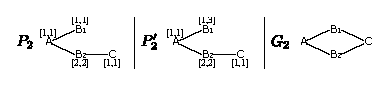
\includegraphics[scale=1.38]{./fig/consistency_motivation.eps}
	\end{center}
	\vspace{-3ex}
	\caption{Pattern satisfiability}
	\vspace{-4ex}
	\label{fig-consistency-example}
\end{figure}

In this section, we first study the pattern satisfiability problem for team formation, then introduce two  two optimization techniques, and finally we present our  batch algorithm for top-$k$ team formation.

% with one novel feature and two optimizations, \ie pattern satisfiability check, and incremental computing for radius varied balls and density based filtering optimization, compared with traditional algorithms for \warn{strong simulation}~\cite{MaCFHW14}.


\subsection{Pattern Satisfiability}
Different from graph simulation \cite{infsimu95} and its extensions \cite{FanLMTWW10,MaCFHW14},
there exist pattern graphs match no data graphs via team simulation, due to the presence of capacity constraints on patterns. We illustrate this with an example.
%\looseness=-1

\begin{example}
\label{exm-consistency}
\ni(1) For pattern $P_2$ in Fig.~\ref{fig-consistency-example},
one can verify that there exist no data graphs $G$ such that $P_2 \eeps G$ because (a) for any nodes $v$ in $G$, if $v$ matches with the node labeled with $B_2$, then it must match with the node labeled with $B_1$, and, hence, (b) the capacity upper bound on $B_1$ should not be less than the lower bound on $B_2$.

\sstab(2) However, pattern $P'_2$ in Fig.~\ref{fig-consistency-example} is satisfiable as $P'_2 \eeps G_2$, and pattern $P_1$ in Fig.~\ref{exm-motivation} is also satisfiable as $P_1 \eeps G_1$.
\end{example}


%Given a pattern $P$, \grouprec firstly checks whether $P$ is satisfiable.

We say that a pattern $P$ is {\em satisfiable} iff there exists a data graph $G$ such that $P$ matches $G$ via team simulation, \ie $P \eeps G$.
The good news is that checking the satisfiability of pattern graphs can be done in low polynomial time.

\begin{prop}
\label{prop-pattern-consistency}
The satisfiability of patterns $P$ can be checked in $O(|P|^2)$ time.
\end{prop}

By treating $P$ as both data and pattern graphs, compute the maximum match relation $M$ in $P$ for $P$, via graph simulation.
Then pattern $P$ is satisfiable iff for each $(u, v)\in M$ with the capacity bounds $[x_u, y_u]$ on $u$ and $[x_v, y_v]$ on $v$, respectively, $x_v \leq y_u$ holds. Observe that the size of $M$ is bounded by $|P|^2$, and pattern graphs are typically small.

By Proposition~\ref{prop-pattern-consistency}, we shall consider  satisfiable pattern graphs only  in the sequel.


\eat{%%%170721
Pattern graphs are typically small, and we only consider  satisfiable patterns in the sequel, by Proposition~\ref{prop-pattern-consistency}.
}%%%170721

\subsection{Batch Algorithm}


\stitle{Handling radius varied balls}. \teamF{} is to find top-$k$ teams within balls $\ball{[v, t]}$, where $v \in V$ and $t \in [1,r]$.
%centered at each node in $G$ with radius $t$ varying from 1 to $r$.
However, it is very costly to construct all $r|V|$ balls, and to compute perfect subgraphs in all of them.
Indeed it is also not necessary, and it only needs to constructs and computes the matches for a number of $|V|$ balls, \ie the set of balls $\ball{[v, r]}$
where $v \in V$ and radius is $r$, and then incrementally computes the perfect subgraphs for balls $\ball{[v, t]}$ ($t \in [1,r-1]$) from the match graphs for ball $\ball{[v, r]}$, as shown below.

\vspace{-1ex}
\begin{theorem}
	\label{thm-tsim-radius}
	Given $P$, ball $\ball{[v, r]}$ and $\ball{[v, t]}$ ($t \in[1,$ $r-1]$) in $G$,
	(1) if $P\eps \ball{[v, t]}$, then $P\eps \ball{[v, r]}$; and
	(2) if $G_s$ (resp. $G'_s$) is the match graph \wrt the maximum match relation $M$ (resp. $M'$) in $\ball{[v, r]}$ (resp. $\ball{[v, t]}$) for $P$ via graph simulation, then $M' \subset M$, and $G'_s$ is a subgraph of $G_s$.	
\end{theorem}
\looseness=-1

When we have the match graph $G_s$ in $\ball{[v, r]}$ for $P$ via graph simulation, to compute the perfect subgraph in $\ball{[v, t]}$ ($t \in [1,r-1]$) for $P$ via team simulation, we need to
(1) first identify the subgraph $G_s^{t}$ in $G_s$ belonging to $\ball{[v, t]}$, which can be easily identified in the process for constructing $\ball{[v, r]}$ without extra computation;
(2) check whether $G_s^{t}$ is already a match graph for $P$ in $\ball{[v, t]}$ via graph simulation; if not, remove the unmatched nodes and edges from $G_s^{t}$ until find the match graph $G'_s$ for $P$ in $\ball{[v, t]}$. This can be achieved by executing an efficient incremental process in~\cite{FanWW13-tods}; and
(3) finally check whether capacity bounds are satisfied. If so, $G'_s$ is the perfect subgraph in $\ball{[v, r]}$ for $P$ via team simulation.

\stitle{Density based ball filtering}. We further reduce the number of balls to speedup the process by adopting the density based filtering technique.
The key idea is to tell whether a ball is possible to produce one of the final top-$k$ matches.

Given a ball $\ball{[v,r]}$, we compute the density upper bound  $\density{\hat{G}_s}$,
where $\hat{G}_s$ is a subgraph of $\ball{[v,r]}$.
If the bound is larger than the density of the current $k$-th result, \ie there is a possibility the for the ball;
Otherwise, the ball is simply ignored to avoid redundant computations.

The trick part is how to efficiently compute the upper bound of $\density{\hat{G}_s}$ for each ball in $G$.
As the best densest subgraph algorithms are in $O(|\ball{[v,r]}|^3)$ time \cite{maximumDenseSubgraph}, which is costly,
we utilize an important result in~\cite{EVMK12}, shown below.



\begin{lemma}
	\label{lemma-approximation-bound}
	Let $\density{H_{c}}$ and $\density{H_{d}}$ be the density of the maximum core  $H_{C}$  and the  densest subgraph $H_{d}$ of graph $H$. Then (1) $\density{H_{c}}\leq \density{H_{d}} \leq 2*\density{H_{c}}$; and (2) there exists an algorithm that computes $\density{H_{c}}$ in $O(|E_H|)$ time~\cite{EVMK12}.
\end{lemma}


Here the maximum core $H_{C}$ of a graph $H$ is a subgraph of $H$ whose node degree is at least $\rho$, where $\rho$ is the maximum possible one. By Lemma~\ref{lemma-approximation-bound}, we use $2*\density{H_{c}}$ as the density upper bound for filtering unnecessary balls.


We are now ready to present our batch algorithm for \teamF{}.

\stitle{Algorithm \grouprec.} As shown in Fig.~\ref{alg-grouprec}, it takes input as $P$, $G$, and two integers $r$ and $k$, and outputs the top-$k$ densest perfect subgraphs in $G$ for $P$.
It firstly checks whether $P$ is satisfiable (line 1).
If so, for each ball $\ball{[v,r]}$ in $G$, it computes the maximum core $\ball{}_{C}$ of $\ball{[v,r]}$, and checks whether the early termination condition holds (lines 3-6).
If so, it returns the current top-$k$ densest perfect subgraphs as top-$k$ teams;
otherwise, it computes the perfect subgraph $G_{s}$ of $P$ in $\ball{[v,r]}$ via team simulation by invoking \rgraphsim (line 7, see full version~\cite{fullvldb18}),
an adaption from graph simulation~\cite{infsimu95,FanLMTWW10} and checking capacity bounds (line 8).
It then computes perfect subgraphs $G'_{s}$ of $P$ in inner balls $\ball{[v,t]}$ by invoking \incsim, an extension of the data incremental algorithms in \cite{FanWW13-tods} and checking capacity bounds (lines 9-11).
%Procedure \rgraphsim is deferred to the appendix, which is an adaption from graph simulation~\cite{infsimu95,FanLMTWW10}.}
%by extending from directed to undirected graphs,  incorporating the capacity constraint check, and only maintaining the capacity bounds satisfied perfect subgraphs.

\stitle{Correctness \& complexity analyses}. The correctness of \grouprec is assured by the following.
%(1) There is a unique perfect subgraph in each ball of $G$.
(1) The correctness of \rgraphsim (resp. \incsim) can be verified along the same lines as for simulation~\cite{infsimu95} (resp. incremental simulation \cite{FanWW13-tods}).
(2) Theorem~\ref{thm-tsim-radius} and Lemma~\ref{lemma-approximation-bound}.
It takes $O(|P|^2)$ to check pattern satisfiability, $O(|V||P||G|)$ to compute team simulation, $O(r|V||V_{P}||E|)$ to incrementally compute matches in inner balls, and $O(|V||E|)$  to compute the density of the maximum core for $|V|$ balls.
Thus \grouprec is in $O(|P|^2+|V||P||G|+r|V||V_{P}||E|)$. However, actual time is much less due to early termination and that  $O(r|V||V_{P}||E|)$ is the worst case complexity for incremental process, while $r$ is small, \ie 2 or 3.



\begin{figure}[t!]
	%\vspace{-2ex}
	\begin{center}
		{\small
			\myhrule
			\vspace{-3ex}
			\mat{0ex}{
				\sstab {\sl Input:\/} $G(V$, $E)$, $P(V_P$, $E_P)$, and positive integers $k, r$.\\
				{\sl Output:\/} Top-$k$ densest teams.\\
				\sstab \bcc \hspace{1ex}\= \If $P$ is unsatisfiable \Then \Return $nil$;\\
				\icc \> $L_{k} := \emptyset$;\\
				\icc \> \For each ball $\ball{[v,r]}$ in $G$ \Do\\
				\icc \>\hspace{2ex}\= compute the maximum core $\ball{}_{C}$ of the ball $\ball{[v,r]}$;\\
				\icc \>\> \If 2*$\density{\ball{}_C} <$  the density of the $k$-th result in $L_{k}$ \Then\\
				\icc  \>\>\hspace{2ex}\= \Return $L_{k}[0:k-1]$;\\
				\icc \>\> $G_s$ := \rgraphsim$(P, \ball{[v,r]})$; \\
				\icc \>\> If $G_s$ satisfy capacity bounds on $P$ \Then Insert $G_s$ into $L_{k}$;\\
				\icc \>\> \For each ball $\ball{[v,t]}$ with $t\in[1,r-1]$ \Do\\
				\icc \>\>\hspace{2ex}\= $G'_s$ := \kw{incSim}$(G_s, P, \ball{[v,t]})$;\\
				\icc \>\>\> If $G'_s$ satisfy capacity bounds on $P$ \Then Insert $G'_s$ into $L_{k}$;\\
				%\icc \>\> \If $\density{G_s}>$ the density of the $k$-th result in $L_{k}$ \Then\\
				%\icc \>\> \If $\density{G_s}>$ the density of $kth$ result in $L_{k}$ and there exists\\
				%     \>\>\hspace{0.5ex}   no $G'_s$ in $L_{k}$ that is same with $G_{s}$ \Then\\
				%\icc \>\>\hspace{2ex}\= remove the $k$-th result in $L_{k}$ and insert $G_s$ into $L_{k}$;\\
				\icc \>\, \Return $L_{k}[0:k-1]$.
			}
			
			\vspace{-4ex} \myhrule
		}
	\end{center}
	\vspace{-3ex}
	\caption{Algorithm \grouprec}
	\label{alg-grouprec}
	\vspace{-4ex}
\end{figure}


\newcommand{\changedinc}{\kw{Changed}}
\newcommand{\cut}{\kw{CUT}}
\newcommand{\imr}{\kw{IMR}}
\newcommand{\imrs}{\kw{IMRs}}
\newcommand{\fb}{\kw{FBM}}
\newcommand{\bs}{\kw{BS}}
\newcommand{\fs}{\kw{FS}}
\newcommand{\bfc}{\kw{BF}}
\newcommand{\upl}{\kw{UP}}
%\newcommand{\fbm}{\kw{FBM}}
\newcommand{\fbmatstruct}{\kw{FBMatStruct}}
\newcommand{\matchindex}{\kw{MatStaIndex}}
\newcommand{\matchimr}{\kw{MatchIMR}}
\newcommand{\for}{\kw{FOR}}
\newcommand{\while}{\kw{WHIlE}}
\newcommand{\allmatch}{\kw{mat}}
\newcommand{\affnode}{\kw{affnode}}

\newcommand{\ms}{\kw{SHOUDfs}}
\newcommand{\ballfilter}{\kw{SHOUDbfc}}

\newcommand{\dens}{\kw{den}}
\newcommand{\identifyaffball}{\kw{IdABall}}
\newcommand{\patedgeinsert}{\kw{patEIns}}
\newcommand{\incmatch}{\kw{IncMatch}}
\newcommand{\wmatchindex}{\kw{wMatStaCode}}
\newcommand{\cflag}{\kw{cflag}}
\newcommand{\dflag}{\kw{dflag}}
\newcommand{\gflag}{\kw{gflag}}
\newcommand{\rflag}{\kw{rflag}}

\newcommand{\incgrpat}{\kw{kPatIncGPM}}
\newcommand{\incgrdata}{\kw{kDataIncGPM}}
\newcommand{\dyngr}{\kw{kDynGPM}}
\newcommand{\affballx}{\kw{AffB}}
\newcommand{\affballsx}{\kw{AffBs}}
\newcommand{\affballacc}{\kw{AffBall^{acc}}}
\newcommand{\affballaccs}{\kw{AffBalls^{acc}}}
\newcommand{\affballimr}{\kw{AffBall^{imr}}}
\newcommand{\affballimrs}{\kw{AffBalls^{imr}}}
\newcommand{\patinc}{\kw{dynamicPG}}
%\newcommand{\patinc}{{\sc dynPG}\xspace}
%\newcommand{\datainc}{{\sc dynDG}\xspace}
\newcommand{\datainc}{\kw{dynamicDG}}
\newcommand{\optpatinc}{\kw{SHOULDoptinc}}
\newcommand{\inc}{\kw{dynamic}}
\newcommand{\matchs}{\kw{R}}
\newcommand{\comb}{\kw{combine}}
\newcommand{\optinc}{\kw{optDynamic}}

\newcommand{\incp}{\kw{dynamicP}}
\newcommand{\incd}{\kw{dynamicG}}


\section{A Unified Incremental Solution}
\label{sec-dynamictopk}

In this section, we first analyze the challenges and design principles of dynamic top-$k$ team formation,
and then develop a unified incremental framework for \dynteamF.
For convenience, the notations used are summarized in Table~\ref{tab-notation}.


\subsection{Analyses of Dynamic Team Formation}


By Theorem~\ref{thm-tsim-radius}, pattern $P$ matches a ball $\ball{[v, t]}$ ($t \in [1,r-1]$), only if $P$ matches ball $\ball{[v, r]}$ via graph simulation,
and the match results for $\ball{[v, t]}$ can be derived from the matches for $\ball{[v, r]}$.
Therefore, the key of the incremental computation is to deal with the balls $\ball{[v, r]}$ with radius $r$.
In the sequel, a ball has a radius $r$ by default.

%Moreover, incremental algorithms typically maintain some auxiliary data structures, which are specifically designed for the update types and need to be maintained by the incremental algorithms. An incremental algorithm for \dyngr should be able to design auxiliary structures to store information needed for both pattern and data increments and maintain it for future ({\em both}) pattern and data increments. This raises even more challenges in designing incremental algorithms for \dyngr, compared to those for \incgrpat and \incgrdata alone.

\eat{%%%EAT
Like data incremental problems, it would be nice to have {\em bounded incremental algorithms}~\cite{Reps96} for pattern incremental problems, which are a class of incremental algorithms whose time complexity depends on the sizes of $P$ and $\changedinc$, which is the changes to the input and output only (\ie $\Delta P$ and the difference between $PG_k(P, G)$ and $PG_k(P\oplus\Delta P, G)$),
and is independent of the size of $G$ and $PG_k(P, G)$.
However, due to the inherent difference between pattern increments and data increments, and the presence of top-$k$ semantic, they are not available for \incgrpat, as shown below.
We say an incremental problem is bounded if it has a bounded incremental algorithm described as above, and is unbounded otherwise.

Similar to the negative results in \cite{FanLMTWW10,FanWW13-tods}

The following results show that even we consider pattern or data increments alone, traditional bounded incremental algorithms are not available for \dyngr already.

%\begin{theorem}
%\label{thm-inc-grouprec-pat}
%$\incgrpat(P,G,k,PG_k(P,G),\Delta P)$ is unbounded, even when
%\bi
%\item $\Delta P$ is
%(a) a single-edge insert,
%(b) a single-edge delete,
%(c) a single-node insert,
%(d) a single-node delete, or
%(e) a single-node-capacity change;
%\item $k$ is 1 or $n$, where $n$ is the number of nodes in $G$.
%\ei
%\end{theorem}
%
%Moreover, due to the presence of top-$k$ semantic, the bounded incremental property is not available for \incgrdata either, as shown below.
%
%\begin{theorem}
%\label{thm-inc-grouprec-data}
%$\incgrdata(P,G,k,PG_k(P,G),\Delta G)$ is unbounded, even when
%\bi
%\item $\Delta G$ is
%(a) a single-edge insert,
%(b) a single-edge delete,
%(c) a single-node insert,
%(d) a single-node delete, or
%\item $k$ is 1 or $n$, where $n$ is the number of nodes in $G$.
%\ei
%\end{theorem}

}%%%EAT

We first analyze the inherent computational complexity of the dynamic top-$k$ team formation.

\stitle{Incremental complexity analysis}. As observed in~\cite{Reps96,inc-survey}, the complexity of incremental algorithms should be measured by the size $|\aff|$ of {\em the changes} in the input and output, rather than the entire input, to measure the amount of work essentially to be performed for the problem.

An incremental problem is said to be {\em bounded} if it can be solved by an algorithm whose complexity is a function of $|\aff|$ alone, and is {\em unbounded}, otherwise. Unsurprisingly, the dynamic top-$k$ team formation problem is unbounded, similar to the other extensions of graph simulation \cite{FanLMTWW10,FanWW13-tods}.


\begin{prop}
\label{thm-inc-grouprec-pat}
The \dynteamF{} problem is unbounded, even for $k$ = 1 and unit pattern or data updates.
\end{prop}


We then illustrate the impact of pattern and data updates on the matching results with an example.


\begin{example}
\label{exm-pattern-challenge}
Continue Example~\ref{exm-motivation-inc} with $\Delta P_1$ and $\Delta G_1$.

% that obviously may introduce new matches.
%For convenience of presentation, we treat $\Delta P_1$ and $\Delta G_1$ separately.

\sstab
(1) For $\Delta P_1$, $\ball{[\kw{PM_1}, 2]}$ already matches $P$, and may produce more matched nodes for $P_1\oplus \Delta P_1$,
thus a re-computation for perfect subgraphs is needed.
For all other balls, $\Delta P_1$ may turn unmatched nodes to matched and may produce perfect subgraphs,
thus re-computation is also needed.

\sstab
(2) For $\Delta G_1$, it produces a new perfect subgraph for $P$ in $G_1\oplus\Delta G_1$,
\ie the connected component having \kw{PM_2}.
%The question is how to directly find new and maintain previous answers without redundant computation.
\end{example}

%\subsection{Analyses of Challenges}
%\label{subsec-challenges}


\begin{table}[tb!]
	%\vspace{-2ex}
	%\vspace{2ex}
	\begin{center}
		\begin{small}
			%\vspace{-2ex}
			\scriptsize
			\begin{tabular}{|c|l|}
				\hline
				{\bf Notations}             &  {\bf Description}     \\
				\hline\hline
				$P,G$                     &  pattern and data graphs       \\ \hline
				$\ball{[v, r]}$              &  a ball in $G$ with center node $v$ and radius $r$  \\ \hline
				$L_k(P, G)$                  &  the list of top-$k$ perfect subgraphs in $G$ for $P$  \\ \hline
				$\Delta P, \Delta G$       &  pattern and data updates       \\ \hline
				$\oplus$                    &  applying updates $\Delta P$ and $\Delta G$ to $P$ and $G$       \\ \hline
				${\cal P}_{h}=\{P_{fi}, C\}$     &  pattern fragmentation: $h$ fragments and cut    \\ \hline
				$\affballsx$                &  affected balls       \\ \hline
				$M(P_{fi}, \ball{[v,r]})$    &  the maximum match relation in $\ball{[v,r]}$ for $P_{fi}$   \\ \hline
				$\tilde{M}(P,G)$            &  fragment-ball matches (auxiliary structure)     \\ \hline
				$\fs$, $\bs$              &  fragment status, ball status (auxiliary structure) \\    \hline
				$\fb$                       &  fragment-ball-match index, containing $\fs, \bs$ \\    \hline
				$\bfc$, $\upl$              &  ball filter, update planner (auxiliary structure) \\    \hline
			\end{tabular}
			\vspace{-1ex}
		\end{small}
		\caption{Notations}
		\label{tab-notation}
		\vspace{-6ex}
	\end{center}
\end{table}


We finally discuss the challenges and principles of designing incremental algorithms for \dynteamF{} from three aspects.

%impacts of pattern and data updates, maintenance of proper auxiliary information, and support of simultaneous pattern and data updates.


\stitle{(1) Impacts of pattern and data updates}.
Beyond Proposition~\ref{thm-inc-grouprec-pat} and Example~\ref{exm-pattern-challenge}, one can also verify that (a) unit pattern updates are likely to result in the entire change in previous results, such that all balls need to be accessed and all matches need to be re-computed,
and (b) the impact of data updates can also be global, such that the entire data graph may need to be accessed to re-compute matches.
Hence, the key is to identify and localize the impacts of pattern and data updates.

%It is rather better to identify the changes in match results in response to data updates, to minimize unnecessary recomputation.
%However, the identification can be difficult and time-consuming.
%It is crucial to identify which parts of $G$ are affected by the data updates and updates match results only within them.
%However, the identification can be difficult and time-consuming.
%The number of affected balls may vary with different data updates.


\stitle{(2) Maintenance of auxiliary information}.
Auxiliary data on intermediate or final results for $P$ in $G$ are typically maintained for incremental computation \cite{Reps96,FanWW13-tods}.
How to design light-weight and effective auxiliary structures is critical.
One may want to store $M(P,G)$, the match relations of $P$ for all balls in $G$,
as adopted by existing incremental pattern matching algorithms for data updates \cite{FanWW13-tods}.
However, the impact of $\Delta P$ is global, as shown in Example~\ref{exm-pattern-challenge}.
By storing $M(P,G)$, for pattern edge/node deletions, it has to recompute matches for all balls, \ie the entire $M(P,G)$.
Thus, storing $M(P,G)$ could be useless, not to mention $L_{k}(P,G)$, the list of top-$k$ perfect subgraphs for $P$ in $G$ \wrt $M(P,G)$.

\stitle{(3) Support of continuous pattern and data updates}.
%Previous research on incremental problems typically focus on increments to the data parts instead of the queries,
%and if exist, the dynamic algorithms either support pattern or data updates, not both of them~\cite{MottinGReform15,FanWW13-tods}.
A practical solution should support continuous pattern and data updates, separately and simultaneously, which further increases difficulties on the design of auxiliary data structures and incremental algorithms.

\subsection{Unified Incremental Framework}
\label{subsec-framework}

Nevertheless, we develop an incremental approach to handling pattern and data updates in a unified framework, by utilizing {\em pattern fragmentation} and {\em affected balls} to localize the impacts of pattern and data updates, and to reduce the cost of maintaining auxiliary structures and computations.

%In light of the challenges, it is desirable to devise a unified efficient incremental approach to handle both $\Delta P$ and $\Delta G$,
%which can reduce the cost for maintaining auxiliary structures and computing final results,
%by restricting the update impacts from global to local.
%Therefore, we propose the {\em dynamic top-$k$ graph pattern matching} model to solve \dynteamF\.
%\looseness=-1

\stitle{(1) Localization with pattern fragmentation}.
We say that \{$P_{f1}(V_{f1},V_{f1})$, $\ldots$, $P_{fh}(V_{fh},V_{fh})$, $C$\} is an {\em $h$-fragmentation} of pattern $P(V_{P}$, $E_{P})$, denoted as ${\cal P}_{h}$,
if (1) $\bigcup_{i=1}^{h}V_{fi}=V_{P}$, (2) $V_{fi}\cap V_{fj} = \emptyset$ for any $i\ne j\in[1, h]$,
(3) $E_{fi}$ is exactly the edges in $P$ on $V_{fi}$, and (4) $C=E_P \setminus (E_{f1}\cup\ldots\cup E_{fh})$.

We also say $P_{fi}$ ($i\in[1,h]$) as a {\em fragment} of $P$, and $C$ as a {\em cut} of $P$, respectively.

Observe that by pattern fragmentation, a pattern update on $P$ is either on a fragment $P_{fi}$ or on the cut $C$ of $P$, and, in this way, the impact of pattern updates is localized. Moreover, graph simulation holds a nice property on pattern fragmentation, as shown below.

\vspace{-0.5ex}
\begin{theorem}
\label{thm-compose}
Let $\{P_{f1},\ldots,P_{fh}\}$ be an $h$-fragmentation of pattern $P$.
For any ball $\ball{}_i$ in $G$, let $M_i$ ($i\in[1,h]$) be the maximum match relation in $\ball{}_i$ for $P_{fi}$ via graph simulation,
and $M$ be the maximum match relation in $\ball{}_i$ for $P$ via graph simulation, respectively,
then $M\subseteq\bigcup_{i=1}^{h}M_{i}$.
\end{theorem}

We also say that $M_i$ is a {\em partial match relation} in ball $\ball{}_i$ for $P$ via graph simulation.
%By Theorem~\ref{thm-compose}, instead of computing $M$ in $\ball{}$ \wrt\ $P$ directly, we can compute $M$ by first computing each $M_i$ in $\ball{}$ \wrt\ $P_{fi}$,
%and then combining them together.
By the nature of graph simulation~\cite{infsimu95}, $\bigcup_{i=1}^{h}M_{i}$ is actually an intermediate result of $M$.
%such that the method above does not incur additional computation cost.
Once we have the maximum match relation $M$ for $P$ in $\ball{}_i$, via graph simulation, we can further produce the result for $P$ in  $\ball{}$ via team simulation, by a capacity check.

That is, based on pattern fragmentation, we maintain
an auxiliary structure for storing fragment-ball matches for incremental computations,
\ie $\tilde{M}(P,G)$ \wrt ${\cal P}_{h}$ that is the maximum match relations for all pattern fragments of $P$ in all balls of $G$, via graph simulation.
Moreover, its space cost is light-weight, as will be shown in the experimental study.
%\revise{
%Moreover, by Theorem~\ref{thm-tsim-radius}, the match results in balls $\ball{[v, t]}$ ($1 \leq t < r$) can be easily derived from the %matches in ball $\ball{[v, r]}$.
%Thus, we only store the maximum match relations for all pattern fragments of $P$ in the balls with radius $r$ of $G$.}
%which will be shown to be much more informative than storing $M(P,G)$ and $L_{k}(P,G)$.
%Its space cost is light-weight, and takes 25MB only, together with all indexes for \citationd that needs 36MB to store itself.


%Indeed, it only takes 25MB and 65MB to store $\tilde{M}(P,G)$ along with all other indexes for Citation and YouTube,  which need 36MB and 114MB, respectively, for storing the entire data graphs.

%We already know that pattern updates $\Delta P$ on $P$ can be treated as the updates $\Delta P$ on $P_{fi}$ or $C$ of $P$.
%If we have cached the maximum match relations of all pattern fragments,
By storing $\tilde{M}(P,G)$, we have $\bigcup_{i=1}^{h}M_{i}$ for each ball $\ball{}$,
and we can simply update $M_i$ while leaving other parts untouched. That is, we indeed compute for $P_{fi}\oplus\Delta P(\ball{})$, instead of $P\oplus\Delta P(\ball{})$, and combine all $P_{fi}\oplus\Delta P(\ball{})$ derive $P\oplus\Delta P(\ball{})$.
Even better, the updates $\Delta P$ on $C$ of $P$ only involve with a simple combination process, avoiding the computation for any pattern fragments.


For a better incremental process, we typically want (1) to avoid skewed updates by balancing the sizes of all fragments, and (2) to minimize the efforts to assemble the partial matches of all fragments.
Thus we define and investigate the {\em pattern fragmentation} problem.

Given pattern $P$ and a positive integer $h$, it is to find
an $h$-fragmentation of $P$ such that both $\max(|P_{fi}|)$ ($i\in[1,h]$) and $|C|$ are minimized.
Intuitively, the bi-criteria optimization problem partitions a pattern into $h$ components of roughly equal size while minimizing the cut size.

\eat{%%%EAT2017-8-2}
Given $P$ and a positive integer $h$, the {\em pattern fragmentation}  problem is to find
an $h$-fragmentation of $P$ such that both $\max(|P_{fi}|)$ ($i\in[1,h]$) and $|C|$ are minimized.
%
Intuitively, we want (1)  to avoid skewed updates by making all fragments roughly the same size and (2) to  minimize the efforts to assemble the partial matches of all fragments.
}%%%EAT2017-8-2

The problem is intractable, as shown below.

\vspace{-0.5ex}
\begin{prop}
	\label{prop-fragmentation}
	The pattern fragmentation problem is \NP-complete, even for $h$ = 2.
\end{prop}



However, $P$ and $h$ are typically small in practice~\cite{FanLMTWW10}, \eg $|P|=15$ and $h=3$.
In light of this, we give a heuristic algorithm, denoted by \kw{PFrag}, for the problem, and is shown in the
full version~\cite{fullvldb18}.
\kw{PFrag} works by connecting pattern fragmentation to the widely studied {\sc $(k, \nu)$-Balanced Partition} problem \cite{AndreevR06},
which is not approximable in general, but has efficient and sophisticated heuristic algorithms~\cite{metis-KarypisK98a}.




\stitle{(2) Localization with affected balls (\affballsx)}.
We further localize the impact of pattern and data updates  with {\em affected balls} to avoid unnecessary computations.


We say that a ball in $G$ is {\em affected} \wrt an incremental algorithm \algorithm{A}, and pattern and data updates,
if \algorithm{A} accesses the ball again.
We use $||\affballsx||$ and $|\affballsx|$ to denote the cardinality and total size of \affballsx, respectively.

%We say that a ball is {\em affected} \wrt an incremental algorithm \algorithm{A} and a set of pattern and data updates if \algorithm{A} re-constructs the ball again using the data graph.

%
Indeed, \affballsx are those balls with a possibility to have final results \wrt $\Delta P$ and $\Delta G$.
We only access \affballsx, and ignore the rest balls.
Specifically, (1) for $\Delta P$, it allows us to avoid computing updated partial relations for an updated fragment in every ball;
and (2) for $\Delta G$, the locality property of team simulation supports to localize the update impacts to a set of balls whose structures are changed by $\Delta G$.
%we just do the computation for the balls whose structure is changed due to $\Delta G$.
\looseness=-1

%\stitle{Remark}. By pattern fragmentation and affected balls, we essentially localize the impact of pattern and data updates from the entire to a fraction of $P$ and from all to a subset of balls in $G$ for team simulation.


%\vspace{-0.5ex}
\stitle{(3) Algorithm framework}. We now provide a unified incremental algorithm to handle both pattern and data updates,
based on pattern fragmentation and affected balls.


Given pattern $P$ with its $h$-fragmentation ${\cal P}_{h}$, data graph $G$, two integers $r$ and $k$,
and auxiliary structures (to be introduced in Section \ref{sec-IncAlg}) such as the partial match relations for all pattern fragments and all balls (radius $r$),
algorithm \inc  consists of three steps for $\Delta P$ and $\Delta G$, as follows.


\etitle{(i) Identifying \affballsx}.
Algorithm \inc invokes two different procedures to identify \affballsx for separate $\Delta P$ or $\Delta G$, respectively.
For  simultaneous $\Delta P$ and $\Delta G$, \inc takes the union of the \affballsx produced by  the two procedures.


\etitle{(ii) Update partial match relations in \affballsx}.
For a ball affected by $\Delta P$, \inc updates the partial match relations for the updated pattern fragments with incremental computation;
For a ball affected by $\Delta G$, \inc updates the partial match relations for all pattern fragments;
And, for a ball affected by both $\Delta P$ and $\Delta G$, \inc follows the same way as $\Delta G$ only.
Meanwhile, auxiliary structure \fb (to be seen shortly) is updated for handling continuous separate and simultaneous pattern and data updates.


\etitle{(iii) Combining partial match relations}. \inc combines all partial relations for a subset of \affballsx and computes the top-$k$ perfect subgraphs within them and their inner balls.


Observe that \inc handles pattern and data updates, separately and simultaneously, in a unified way.



%%%%%%%%%%%%%%%%%%%%%%%%%%%%%%%%%%%%%%%%%%%%%%%%%%%%%%%%%%%%%%%%%%%%%%%%%%%%%%%%%%%%%%%%%%%%%%%%%%%%
\eat{%%%EAT
Theorem~\ref{thm-inc-grouprec-pat} and ~\ref{thm-inc-grouprec-data} show that, conventional bounded incremental algorithms are not available for $\incgrpat$ and $\incgrdata$ even for unit update only.
The main reasons are three challenges introduced by pattern/data incremental and the top-$k$ semantic, summarized as follows.

\sstab {\bf Challenge (1): impacts of pattern or data changes}.
The first challenge is how to identify and restrict, if possible, the impacts of pattern or data changes. This is nontrivial.
(a) Due to the nature of pattern changes, a unit update on pattern graph may have impact on all perfect graphs in $PG(P,G)$, or even add new matches. Indeed, for any algorithm takes input as $P$, $G$, $k'$, $PG_k(P,G)$ and $\Delta P$, it has to access entire $G$ (every ball in $G$), even when $\Delta P$ is a unit update, $k' = 1$ and $k = |V_G|$. That is, the impacts of a pattern update can be global.
(b) Data changes may also cause complicated impacts on both the ball structures and the number of balls in $G$. For one thing, the number of balls in $G$ may increase or decrease with new data changes; for another, the match relations in existing balls may have to be re-computed since the structure of balls may change.
These impacts may vary over updates, and require us to identify them.
% the number of balls used by the TEAM simulation, and the
% For data changes, an edge/node delete (insert) may turn a matched node unmatched (unmatched node matched). We need to recompute new matches for all balls when we do not know which balls will contain matches due to the structure changes.

\sstab {\bf Challenge (2): necessary auxiliary information}.
The second challenge comes from the uninformative in the output top-$k$ perfect graphs of the team simulation.
(a) Due to the top-$k$ semantics, $PG_k(P,G)$ contains only top-$k$ perfect graphs \wrt match relations in $M(P,G)$, which could be extremely uninformative even when $k$ is large, as any changes in the results may requires the knowledge of all perfect graphs to enforce the top-$k$ semantics.
(b) Worse still, for pattern changes, even all perfect subgraphs $PG(P,G)$ are precomputed and cached, it can provide no help for pattern incremental when there are pattern edge/node deletes, as indicated in example~\ref{exm-pattern-challenge}.
(c) Traditional incremental algorithms typically maintain some auxiliary data structures to accelerate the incremental process. However, the physical storage is limited in practice, and essential structures needed for team simulation may not be able to fit in the storage budget.
Indeed, we examined basic structures for team simulation and using real-life data to validate whether they are suitable as auxiliary structures.
%
(i) The first candidate is the balls, since balls of the data graph are the basic computation unit for team simulation. We test the cost of cache them. The results are discouraging.
It will take about 361GB, 437GB and 222GB for Citation, YouTube and Synthetic data ($10^7$ nodes) when $r$ is set to 3, and 338GB, 420GB and 222GB even when compression technique is adopted. This shows that precomputing and caching all balls in $G$ as auxiliary information is impractical.
(ii) Another choice is to precompute and store $M(P,G)$, as adopted by some pattern incremental algorithms~\cite{FanWW13-tods}.
However, as indicated in Challenge (1), the impact of $\Delta P$ is global. By storing $M(P,G)$, for edge/node inserts or capacity changes, the incremental process can get match results by updating all matches in $M(P,G)$ for all balls in $G$; worse still, for edge/node deletes, it has to recompute all matches in $M(P,G)$ for all balls in $G$. Therefore, storing $M(P,G)$ cannot improve the incremental process in many cases, worst still, it even takes extra cost to maintain $M(P,G)$.
}%%%EAT


%%%%%%%%%%%%%%%%%%%%%%%%%%%%%%%%%%%%%%%%%%%%%
\begin{figure*}[tb!]
	\begin{center}
		\subfigure{\label{fig-auxstr-index}
			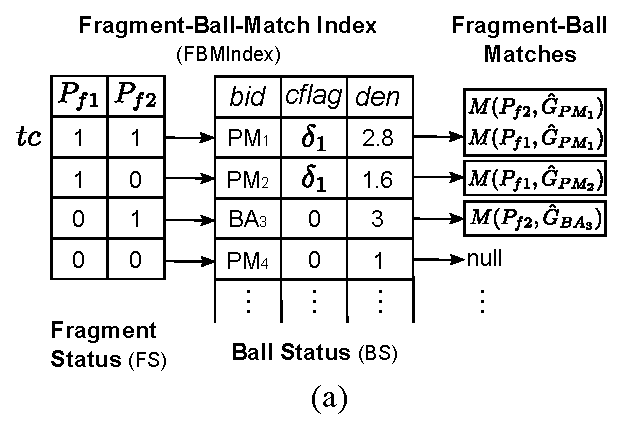
\includegraphics[scale=0.585]{./fig/fig-auxstr-index.eps}}
		\subfigure{\label{fig-inc-maintain-unit}
			\quad\quad \vrule \quad\quad
			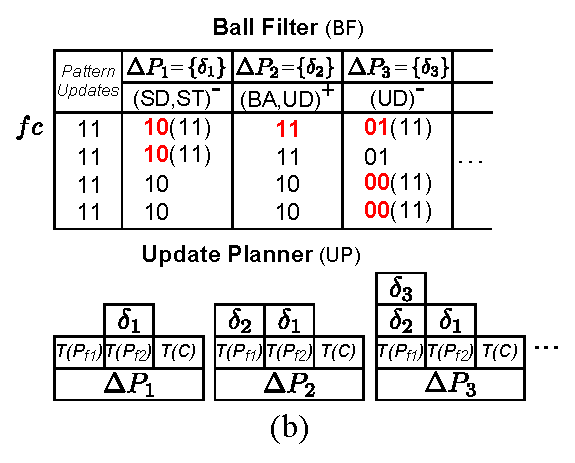
\includegraphics[scale=0.585]{./fig/fig-inc-maintain-unit.eps}}
		\subfigure{\label{fig-inc-maintain-batch}
			\vrule \quad\quad
			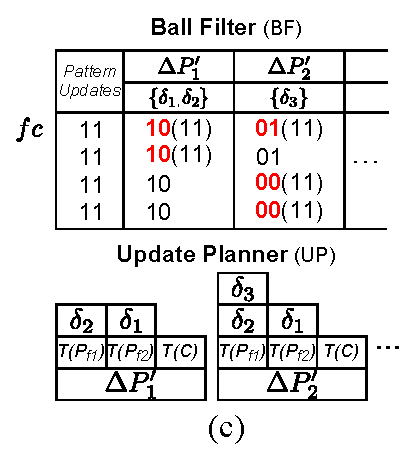
\includegraphics[scale=0.585]{./fig/fig-inc-maintain-batch.eps}}
		\vspace{-2ex}
		\caption{Example auxiliary data structures}
		\label{fig-auxiliary-structures}
		\vspace{-4ex}
	\end{center}
\end{figure*}
%%%%%%%%%%%%%%%%%%%%%%%%%%%%%%%%%%%%%%%%%%%%%

\section{Incremental Algorithms}
\label{sec-IncAlg}

In this section, we introduce the details of our incremental algorithm \inc, including (a) auxiliary data structures,
(b) algorithms \incp and \incd to handle pattern and data updates, respectively, and (c) \inc by integrating \incp and \incd together.
%We finally unify pattern and data updates by integrating \incp and \incd together.

\subsection{Auxiliary Data Structures}
\label{subsec-auxstr}

Auxiliary structures fall into two classes:
maintain partial matches and handle pattern incremental computing. Consider an $h$-fragmentation \{$P_{f1}, \ldots, P_{fh}, C$\} of pattern $P(V_P, E_P)$, data graph $G(V, E)$, and pattern updates $\Delta P$.

\vspace{0.5ex}
(I) Data structures in the first class are as follows.

\etitle{(1) Fragment status (\fs)} consists of $2^h$ boolean vectors $(b_1,\ldots,b_h)$, referred to as {\em type code (tc)}, where $b_i$ $(i\in [1,h])$ is either 0 or 1. Recall that $h$ is very small, \eg 3.

We use \fs to classify the match status of balls in $G$ into $2^h$ types \wrt ${\cal P}_h$.
For a ball with type code $(b_1,\ldots,b_h)$, $b_i$ is 1 iff $P_{fi}$ matches the ball via graph simulation.

\vspace{0.4ex}
\etitle{(2) Ball status (\bs)} consists of $|V|$ triples $(bid, cflag, den)$, such that $bid$ is the $id$ of a ball,
$cflag$ is the id of the latest processed unit pattern update for the ball (initially set to $0$),
and $den$ is the density upper bound of subgraphs in the ball.
\looseness=-1

We use \bs to store the basic information for balls in $G$.

\vspace{0.4ex}
\etitle{(3) Fragment-ball matches} of $P$ in $G$, denote as $\tilde{M}(P,G)$,
are $\bigcup_{i\in[1,h], v\in V} M(P_{fi},\ball{[v,r]})$,
such that $M(P_{fi},\ball{[v,r]})$ is the maximum match relation for $P_{fi}$ in ball $\ball{[v,r]}$, via graph simulation,
and there are in total $|V|$ balls.

Here $\tilde{M}(P,G)$ is used to store match relations for the pattern fragments of $P$ in all balls of $G$. Instead of storing a single $\tilde{M}(P, G)$, we organize $\tilde{M}(P, G)$ in terms of the match status between pattern fragments and balls, \ie\ \fs and \bs.

\vspace{0.4ex}
\etitle{(4) Fragment-ball-match index (\fb)} links \fs and \bs together, to form the {\em fragment-ball-match index}. Then \fb is linked to $\tilde{M}(P,G)$. \revise{The details are shown below.}

For each record of ball $\ball{[v,r]}$ in \bs, (a) there is a link from its type code in \fs pointing to the record; and
(b) there is another link from the record to a set of $M({P}_{fi}, \ball{[v,r]})$ $(i\in [1,h])$ in $\tilde{M}(P,G)$,
if the type code with which the ball is associated has $b_i = 1$, \ie $M({P}_{fi}, \ball{[v,r]})$ is not empty.

Intuitively, \fb indexes the partial match relations $\tilde{M}(P,G)$ based on the match status of balls \wrt ${\cal P}_h$.




\begin{example}
\label{exa-matchindex}
Consider $P_1$ and $G_1$ (both without dashed edges) in Fig.~\ref{exm-motivation}, $r=2$, $k=2$, $h=2$,
auxiliary structures $\tilde{M}(P,G)$ and \fb\,that are shown in Fig.~\ref{fig-auxiliary-structures}(a).
$P_1$ is divided into fragments $P_{f1}$ and $P_{f2}$ by algorithm \kw{PFrag},
so there are $2^2=4$ type codes in \fs.
For balls linked with $tc$ $(1, 1)$, \eg ball $\ball{[\kw{PM_1},2]}$,
there are matches to both $P_{f1}$ and $P_{f2}$ in the ball.
Besides, there exist balls $\ball{[\kw{PM_2},2]}$, $\ball{[\kw{BA_3},2]}$ and $\ball{[\kw{PM_4},2]}$
linked with $tc$ $(1, 0)$, $(0, 1)$ and $(0, 0)$ respectively.
We only consider these 4 balls in the sequel.
\end{example}

%Algorithm \inc uses \fb in step (1) and $\tilde{M}(P,G)$ in step (2), and updates both of them in step (2).

\vspace{0.5ex}
(II) Data structures in the second class are as follows.

\vspace{0.5ex}
\etitle{(1) Ball filter  (\bfc)} consists of $2^{h}$ boolean vectors $(b_1$, $\ldots$, $b_h)$, referred to as {\em filtering code (fc)},
such that each $fc$ in \bfc corresponds to a type code $tc$ in \fs.
Each $b_i$ $(i\in [1, h])$ in an $fc$ of \bfc is initially set to $1$,
and is updated for each unit pattern update $\delta$ in $\Delta P$:
(a) when $\delta$ is an edge deletion or a node deletion to ${P}_{fi}$,
the $i$-th bit of all the $2^{h}$ filtering codes in \bfc is set to $0$; Otherwise, (b) \bfc remains intact.


%Algorithm \inc updates and uses \bfc in step (1) for identifying \affballsx for pattern updates.
\vspace{0.5ex}
\etitle{(2) Update planner (\upl)} consists of $h+1$ stacks $T({P}_{f1})$, $\ldots$, $T({P}_{fh})$, $T(C)$.
Stack $T(P_{fi})$ $(i\in [1,h])$ (resp. $T(C)$) records all unit updates in all arrived pattern updates $\Delta P_1$, $\ldots$, $\Delta P_{N}$ that are applied to fragment $P_{fi}$ (resp. $C$) of $P$.
Initially, all of them are empty.
They are dynamically updated for each unit update in each set of coming pattern updates.
\looseness=-1

%Algorithm \inc updates \upl in step (1) to organize and accumulate unit pattern updates to pattern fragments, and uses \upl in step (2) to update $\tilde{M}(P,G)$ in \affballsx.


%More specifically, we use (a) {\em fragment-ball status index} and (b) {\em ball status index} to organize $\tilde{M}(P, G)$ in terms of the match status between balls and pattern fragments. We then link them to the fragment-ball matches, to form an integrated organization of $\tilde{M}(P, G)$, called {\em fragment-ball math struct}, denoted by \fb.




\subsection{Dealing with Pattern Updates}
\label{subsec-Qinc}

We present algorithm \incp to handle pattern updates $\Delta P$, followed the steps in Section~\ref{sec-dynamictopk}, and
an early return optimization technique for \incp.
%Note that for any $h$-fragmentation ${\cal P}_h$ of $P$, $|{\cal P}_h|$ = $|P|$.




%\ie identifying \affballsx (Section~\ref{subsubsec-affball}), updating $\tilde{M}(P,G)$ within \affballsx (Section~\ref{subsubsec-updtm}), and combining to get final results (Section~\ref{subsubsec-combine}).






\subsubsection{Identifying Affected Balls}
\label{subsubsec-affball}

We first develop procedure \identifyaffball to identify \affballsx,
which utilizes auxiliary structures \fb and \bfc.

\stitle{Procedure \identifyaffball}.
Given an $h$-fragmentation ${\cal P}_{h}$ of $P$, $\Delta P$,
(1) it updates \bfc by processing all unit updates in $\Delta P$.
(2) For each $i\in [1, 2^h]$, it then executes a bitwise \kw{AND} operation (\&) between type code $tc_i$ of \fs in \fb and updated $fc_{i\Delta}$ in \bfc, \ie $tc_i\& fc_{i\Delta}$.
(3) Finally, if $tc_i\& fc_{i\Delta} = fc_{i\Delta}$, \identifyaffball refers to \bs in \fb to mark the balls with type code $tc_i$ as \affballsx, and resets $fc_{i\Delta}$ to $(1, \ldots, 1)$.


%If there exists a single-edge delete on pattern fragments or single-node insert/delete in $\Delta P$, then \identifyaffball returns all such \affballsx as \affballaccs. Intuitively, \affballsx are those balls that may contain new matches due to the pattern updates, while \affballaccs are those ones that cannot be computed from $P$ and $\tilde{M}(P,G)$ due to node inserts/deletes or edge deletes on pattern fragments in $\Delta P$.


\begin{example}
\label{exa-identifyaffball}
Consider the input and auxiliary structures in Example~\ref{exa-matchindex}, and \bfc in Fig.~\ref{fig-auxiliary-structures}.

\sstab(1) $\Delta P_1$ comes with a unit edge deletion $\delta_1$=$(\kw{SD},$ $\kw{ST})^-$ on $P_{f_2}$, and
\bfc is updated accordingly as shown in the second column of \bfc in Fig.~\ref{fig-auxiliary-structures}(b).

\identifyaffball first identifies balls with type code $(1, 1)$ and $(1, 0)$ as \affballsx,
\ie $\ball{[\kw{PM_1},2]}$ and $\ball{[\kw{PM_2},2]}$, and then \identifyaffball resets the two corresponding filtering codes in \bfc to $(1, 1)$.


\sstab(2) Consider another case when $\Delta P'_1$ comes with $\delta_1$ and $\delta_2$, where $\delta_1$ is same as above and $\delta_2 = (\kw{BA},\kw{UD})^+$. \bfc is updated as shown in the second column of \bfc in Fig.~\ref{fig-auxiliary-structures}(c), and \identifyaffball identifies the same \affballsx as above.
\end{example}

In real-life networks, the quantity of balls with type code ($0,\ldots,0$) is several orders of magnitude larger than that of balls who match with at least one pattern fragment. By filtering out balls with \eg $tc$ = ($0,\ldots,0$) or ($1,0,\ldots,0$),
it can reduce a large amount of redundant computations.


\begin{prop}
\label{prop-canaffballs}
For any ball $\ball{[v,r]}$ in $G$, if there exists a perfect subgraph of $P\oplus \Delta P$ in $\ball{[v,r]}$,
then $\ball{[v,r]}$ must be an affected ball produced by procedure \identifyaffball.
\end{prop}

%The proof is deferred to the full version~\cite{fullvldb18}.


%\vspace{1ex}
\stitle{Lazy update policy}. To reduce computation, \incp only updates the partial relations for \affballsx in $\tilde{M}(P,G)$ for computing  $L_k(P\oplus \Delta P, G)$.
%However, the filtered balls are still in need for handling future pattern updates $\Delta P'$,
%and their partial match relations are outdated \wrt $P\oplus \Delta P$.
However, those partial relations in the filtered balls also needs an update for handling future updates $\Delta P'$, but
definitely become outdated \wrt $P\oplus \Delta P$.
Hence, \incp needs a smart policy to maintain those match relations in the filtered balls.
%$L_k(P\oplus \Delta P \oplus \Delta P', G)$ even though $\tilde{M}(P,G)$ are not updated entirely for all balls.


To do this, algorithm \incp maintains the status of all unit updates applied to $P$ so far, and processes unit updates in $\Delta P$ as {\em late} as possible, while having no effects on future updates $\Delta P'$, \ie a {\em lazy update policy}.
%In other words, the match results for each $\Delta P$ can be returned as {\em early} as possible.

Algorithm \incp utilizes auxiliary structure \upl together with the $cflag$ item in \bs.
When handling current $\Delta P$, for each ball $\ball{}$, $\ball{}[\kw{cflag}]$ records the id of the latest processed unit pattern update for $\ball{}$, and is initialized to $0$.
When future $\Delta P'$ comes, for any \affballx $\ball{}$ \wrt $\Delta P'$ and any fragment $P_{fi}$,
\incp computes $M(P_{fi}\oplus\Delta P'_{fi}, \ball{})$ based on $M(P_{fi}, \ball{})$ by procedure \incmatch (to see in Section~\ref{subsubsec-updtm}),
where $\Delta P'_{fi}$ consists of the unit updates stored in $T(P_{fi})$ whose ids are larger than $\ball{}[\kw{cflag}]$ in \bs.




\begin{example}
\label{exa-lazyupdate}
Continue Example~\ref{exa-identifyaffball}.
(1) Balls $\ball{[\kw{PM_1},2]}$ and $\ball{[\kw{PM_2},2]}$ are \affballsx, and
\upl is shown in Fig.~\ref{fig-inc-maintain-unit}.

\sstab(a) \upl is updated \wrt\ $\Delta P_1=\{\delta_1\}$.
\incp updates the partial relations for $P_{f2}$ \wrt\ $\delta_1$ in the two balls,
and sets their $cflag$ in \bs to $\delta_1$, as the status shown in Fig.~\ref{fig-auxstr-index}.

\sstab
(b) Afterwards, $\Delta P_2$ with an edge insertion $\delta_2 = (\kw{BA},\kw{UD})^+$ comes.
\identifyaffball updates \bfc and \upl as shown in Fig.~\ref{fig-inc-maintain-unit} and identifies balls with $tc$ $(1, 1)$ as \affballsx, \eg $\ball{[\kw{PM_1},2]}$.

\sstab
(c) Finally, $\Delta P_3$ with a node deletion $\delta_3$ = $(\kw{UD})^-$ comes.
\identifyaffball identifies $tc$ $(1, 1)$, $(0, 1)$ and $(0, 0)$ as \affballsx.
Take ball $\ball{[\kw{BA_3}, 2]}$ for example, which is the first time identified as an \affballx.
By referring to \upl, \incp updates the partial relations for $P_{f1}$ \wrt\ $\{\delta_2, \delta_3\}$,
and for $P_{f2}$ \wrt\ $\{\delta_1\}$.
\looseness=-1


\sstab
(2) In the case when $\Delta P'_i$ contains multiple\eat{unit} updates, \bfc and \upl are updated accordingly as shown in Fig.~\ref{fig-auxiliary-structures}(c).
\end{example}

\vspace{-.5ex}


\subsubsection{Updating Fragment-Ball Matches}
\label{subsubsec-updtm}

We then update the partial match relations for \affballsx in $\tilde{M}(P,G)$ \wrt $\Delta P$,
by procedure \incmatch.


\stitle{Procedure \incmatch}. Given $h$-fragmentation ${\cal P}_{h}$ of $P$, $G$, $\tilde{M}(P,G)$, $\Delta P$, \upl and \affballsx \wrt $\Delta P$.
\incmatch updates $M(P_{fi}, \ball{})$ to $M(P_{fi}\oplus\Delta P_{fi}, \ball{})$ in $\tilde{M}(P,G)$ for each fragment $P_{fi}$ and each \affballx $\ball{}$.
Recall that $\Delta P_{fi}$ consists of unprocessed unit updates accumulated in \upl applied to $P_{fi}$.
%Recall that $\Delta P_{fi}$ consists of the unit updates in $\Delta P$ applied to $P_{fi}$ we get from \upl.
We show how to update $M(P_{fi}, \ball{})$ in different cases.



%\eetitle{(1) Capacity changes in $\Delta P_{fi}$ or updates on $C$ only}.

\eetitle{(1) There exist edge/node deletions in $\Delta P_{fi}$}.
In this case, \incmatch accesses the \affballx $\ball{[v,r]}$ in $G$.
It simply computes the maximum match relations for $P_{fi}\oplus \Delta P_{fi}$ in $\ball{[v,r]}$
by procedure \rgraphsim in $O(|P_{fi}\oplus \Delta P_{fi}||\ball{[v,r]}|)$ time.

\eetitle{(2) No edge/node deletions in $\Delta P_{fi}$}.
\incmatch processes updates of the same type together in this case.

\eetitle{(2).i Capacity changes in $\Delta P_{fi}$ or updates on $C$}.
In this case, no computation is needed for maintaining \revise{partial relations for} \affballsx at all,
\ie $M(P_{fi}\oplus\Delta P_{fi}, \ball{}) = M(P_{fi}, \ball{})$.
\warn{Only a capacity check and an inner ball results check in the combination procedure are needed} (to see in Section~\ref{subsubsec-combine}).


%It is same for the updates on cut edges $C$ of ${\cal P}_{h}$ of $P$, which are also processed by the combination procedure.


%\eetitle{(3) Edge insertions in $\Delta P_{fi}$ only}.
\eetitle{(2).i Edge insertions in $\Delta P_{fi}$}.
In this case, \incmatch calls procedure \patedgeinsert to process edge insertions.
% $|\Delta P_{fi}|$ times.



\begin{figure}[t!]
%\vspace{-2ex}
\begin{center}
{\small
\myhrule
\vspace{-2ex}
\mat{0ex}{
\sstab {\sl Input:\/} $M(P_{fi}, \ball{[v,r]})$, $\ball{[v,r]}$, pattern edge insertion $\delta$ = $(u,u')^+$.\\
{\sl Output:\/} $M(P_{fi}\oplus \delta, \ball{[v,r]})$.\\
\sstab \bcc \hspace{1ex} \= $\kw{RMv}:=\emptyset$;\\
\icc \> \For \Each $u \in V_{P}$ \Do $\matchs(u)$ := \{$w | (u,w) \in M(P_{fi}, \ball{[v,r]})$\};\\
\icc \> \For \Each node $w \in \matchs(u)$\eat{in $M(P_{fi},\ball{[v,r]})$} \Do\\
\icc \>\hspace{2ex}\= \If there exists no $(w, w')\in E_{\ball{[v,r]}}$ with $w' \in \matchs(u')$ \Then\\
\icc \>\>\hspace{2ex}\= $\kw{RMv}.\kw{push}([u,w])$;\\
\icc \> \For \Each node $w' \in \matchs(u')$\eat{$M(P_{fi},\ball{[v,r]})$} \Do\\
\icc \>\> \If there exists no $(w', w)\in E_{\ball{[v,r]}}$ with $w \in \matchs(u)$ \Then\\
\icc \>\>\> $\kw{RMv}.\kw{push}([u',w'])$;\\
\icc \> \While $\kw{RMv}\neq \emptyset$ \Do\\
\icc \>\hspace{2ex}\= $[u,w]:=\kw{RMv}.\kw{pop}$(); $\matchs(u):=\matchs(u)\setminus\{w\}$;\\
\icc \>\> \For \Each $(u,u')\in E_{P_{fi}}$ \Do\\
\icc \>\>\hspace{2ex}\= \For \Each $(w, w')\in E_{\ball{[v,r]}}$ with $w' \in \matchs(u')$ \Do\\
\icc \>\>\>\hspace{2ex}\= \If there is no $(w', w'')\in E_{\ball{[v,r]}}$ with $w'' \in \matchs(u)$ \Then\\
\icc \>\>\>\>\hspace{2ex}\= \kw{RMv}.\kw{push}([$u',w'$]);\\
\icc \> \If there is a node $u\in V_{P_{fi}}$ with $|\matchs(u)| = 0$ \Then $\matchs(\cdot):=\emptyset$;\\
\icc \> $M(P_{fi}\oplus \delta, \ball{[v,r]})$ := \{$(u,w) | u \in V_{P}, w \in \matchs(u)$\};\\
\icc \> \Return $M(P_{fi}\oplus \delta, \ball{[v,r]})$;
}
\vspace{-2.5ex} \myhrule
}
\end{center}
\vspace{-3ex}
\caption{Procedure \patedgeinsert} \label{alg-patedgeinsert}
\vspace{-4ex}
\end{figure}


\stitle{Procedure \patedgeinsert}.
Given $M(P_{fi}, \ball{[v,r]})$ (also represented by $\matchs(\cdot)$), $\ball{[v,r]}$ and an edge insertion $\delta=(u,u')$, \patedgeinsert computes $M(P_{fi}\oplus\delta, \ball{[v,r]})$ {\em incrementally}, as shown in Fig.~\ref{alg-patedgeinsert},
along the same lines as for data incremental graph simulation~\cite{FanWW13-tods}.
\patedgeinsert first finds the directly affected data nodes which need to be removed from $\matchs(\cdot)$ due to the edge insertion to $P_{fi}$,
and pushes them along with the matched pattern nodes into $\kw{RMv}$ (lines 3-8).
It then recursively identifies and removes the nodes in $\matchs(\cdot)$ affected by the previous removed nodes (lines 9-14).
The recursive process is executed by utilizing a stack $\kw{RMv}$.
If there exists a pattern node $u$ with empty $\matchs(u)$, then $\matchs(\cdot)$ is set to $\emptyset$ (line 15).
Finally, \patedgeinsert returns the updated $\matchs(\cdot)$ for $P_{fi}\oplus \delta$ (lines 16-17).
\looseness=-1


\begin{example}
\label{exa-edge-insertion}
Consider case (1)-(b) in Example~\ref{exa-lazyupdate}.
Given $\delta_2 = (\kw{BA},\kw{UD})^+$, and $M(P_{f1}, \ball{}_{\kw{PM_1}})$, which is composed of nodes \kw{PM_1}, \kw{BA_1} and \{\kw{UD_1},\kw{UD_2}\} mapped to nodes \kw{PM}, \kw{BA} and \kw{UD} in $P_{f1}$.
To compute the updated $M(P_{f1}\oplus \delta_2, \ball{}_{\kw{PM_1}})$,
\patedgeinsert removes \kw{UD_2} which is directly affected by $\delta_2$, and finds no other nodes need to be removed.
\end{example}

%When update the partial match relations for fragment $P_{f2}$ \wrt\ $\delta_2 = (\kw{BA},\kw{UD})^+$ in ball $\ball{[\kw{PM_1},2]}$,
%and $M(P_{f2}, \ball{[\kw{PM_1},2]})$ is composed of nodes \kw{PM_1}, \kw{BA_1} and \{\kw{UD_1},\kw{UD_2}\}
%mapped to nodes \kw{PM}, \kw{BA} and \kw{UD} in $P_1$,
%\patedgeinsert removes \kw{UD_2} which is directly affected by $\delta_2$,
%and finds no other nodes need to be removed.


%\eetitle{(4) Node insertions in $\Delta P_{fi}$ only}.
\eetitle{(2).ii Node insertions in $\Delta P_{fi}$}.
Node insertions are handled in the same way as edge insertions, by extending \patedgeinsert.

Given a node insertion $\delta$ = $(u,(u,u'))^+$, where $u$ is a newly inserted node,
to compute the updated $M(P_{fi}\oplus \delta, \ball{[v,r]})$,
\incmatch firstly computes the set of nodes $\matchs(u)$ in $\ball{[v,r]}$ which have the same label with $u$, and then calls \patedgeinsert($M(P_{fi}, \ball{[v,r]})$, $\ball{[v,r]}$, $(u,u')$) to get the updated result.

\vspace{0.5ex}
\stitle{Updating \fb.} After updating $\tilde{M}(P,G)$,
\incp updates \fb for all \affballsx, by changing the links according to the updated partial relations in $\tilde{M}(P,G)$, and also updating the \kw{cflag} item in \bs, which is in $O(||\affballsx||)$ time.


\subsubsection{Combining Fragment-Ball Matches}
\label{subsubsec-combine}

Algorithm \incp finally combines the updated partial match relations in \affballsx to get the updated top-$k$ perfect subgraphs $L_{k}(P\oplus \Delta P,G)$ by procedure \comb. Observe that only the balls from \affballsx which match with all pattern fragments of $P\oplus \Delta P$ can enter the combination process.



\stitle{Procedure \comb}. For an \affballx $\ball{[v,r]}$, \comb invokes $\patedgeinsert(\bigcup_{i\in [1, h]}M(P_{fi},\ball{[v,r]}), \ball{[v,r]}, C\oplus \Delta C)$
to compute the maximum match relations of $P\oplus \Delta P$ for $\ball{[v,r]}$ incrementally,
where $\Delta C$ consists of the edge insertions/deletions in $\Delta P$ applied to the cut edges $C$.
It then checks whether the capacity bounds, together with the updates on them, are satisfied.
If so, it constructs the perfect subgraph \wrt the match relations above.
\warn{It then checks the inner balls results together with the capacity bounds} and finally returns the list of top-$k$ perfect subgraphs $L_{k}(P\oplus \Delta P,G)$.



\begin{example}
\label{exa-combination}
Continue Example~\ref{exa-lazyupdate}-(1), after \incp updated partial relations for \affballsx \wrt $\Delta P_3$,
balls $\ball{[\kw{PM_1},2]}$, $\ball{[\kw{PM_2},2]}$ and $\ball{[\kw{BA_3},2]}$ enter the combination process.

\sstab
(1) For $\ball{[\kw{PM_1},2]}$ and $\ball{[\kw{PM_2},2]}$, as $C\oplus \Delta C=\{(\kw{PM},\kw{SA})\}$,
\comb finds that there is an \kw{SA_i} (resp.\,\kw{PM_j}) connecting to \kw{PM_j} (resp.\,\kw{SA_i}),
and the capacity bounds are satisfied.
\warn{For inner balls, based on above results, \comb finds that no perfect subgraphs reside in $\ball{[\kw{PM_1},1]}$ and $\ball{[\kw{PM_2},1]}$.}
Hence it returns above two perfect subgraphs in two balls.

\sstab
(2) For $\ball{[\kw{BA_3},2]}$, \comb finds no \kw{SA_i} connecting to \kw{PM_j}, and vice versa.
\warn{So no results are in it and its inner balls.}
\end{example}


\subsubsection{Early Return Optimization Technique}
\label{subsubsec-Inc-opt}


%As introduced in last section, the {\em lazy update manner} accelerates the process to return updated top-$k$ perfect subgraphs by postponing the processing of each unit pattern update.
We propose an optimization technique for \incp to further speed-up the incremental computations, by making use of the top-$k$ semantics.
%
We first define {\em early return} for incremental top-$k$ algorithms, analogous to {\em early termination} for batch top-$k$ algorithms~\cite{FaginLotem03}.


\stitle{Early return}. An algorithm has the {\em early return property},
if for pattern $P$ with updates $\Delta P$ and for any data graph $G$,
it outputs $L_k(P\oplus \Delta P, G)$ as early as possible without the need to update match relations for every \affballx,
while the updates can be executed in background.


\begin{prop}
\label{prop-early-return}
There exists an algorithm for the dynamic top-$k$ team formation problem with early return property.
\end{prop}


We prove \incp retains the early return property.
Recall the density based filtering optimization for algorithm \optgrouprec in Section~\ref{sec-tsimAlg}.
\incp also utilizes density upper bounds for pruning a portion of \affballsx.
More specifically, given $P$ and $G$, \incp maintains the density upper bound for each ball in the $den$ item in \bs, \ie $\ball{}[\kw{den}]$,
calculated according to Lemma~\ref{lemma-approximation-bound}.
Thus, given $\Delta P$, if the top-$k$ densest perfect subgraphs found so far are denser than the density upper bound of the remaining \affballsx,
\incp\ {\em outputs} the current top-$k$ densest perfect subgraphs as $L_k(P\oplus \Delta P, G)$,
while continuing updating $\tilde{M}(P, G)$ in \affballsx in {\em background}.

Note that the early return optimization is  effective for pattern updates, but not for data updates and the case when $\Delta P$ contains node insertions with new labels (expertise).

\begin{figure}[t!]
	%\vspace{-2ex}
	\begin{center}
		{\small
			\myhrule \vspace{-2ex}
			\mat{0ex}{
				\sstab {\sl Input:\/} \= $P$, $h$-fragmentation ${\cal P}_{h}$, $G$, integers $r$ and $k$, $\Delta P$, and\\
				\>auxiliary structures $\tilde{M}(P,G)$, \fb, \bfc and \upl.\\
				{\sl Output:\/} Top-$k$ perfect subgraphs for $P \oplus \Delta P$ in $G$.\\
				\sstab \bcc \hspace{1ex} \= $L_{k}$ := $\emptyset$;\\
				\icc \> \affballsx\ :=  $\identifyaffball({\cal P}_h, \Delta P, \fb, \bfc)$;\\
				\icc \> Sort \affballsx by $\ball{}[\kw{den}]$ in non-ascending order;\\
				\icc \> \For \Each $\ball{[v,r]}$ in \affballsx \Do\quad/* non-ascending order */\\
				\icc \> \hspace{3ex} \= \If $|L_{k}| \geq k$ \And $\ball{[v,r]}[\kw{den}] \leq \density{L_{k}[k]}$ \Then \\
				\icc \>\>\hspace{2ex} \= \bf{Output} $L_{k}[0:k-1]$.\quad/* early-return optimization*/\\
				%/* Running in background after returning top-$k$ results for $\Delta P$ */\\
				\icc \>\>$\incmatch(M(P_{fi},\ball{[v,r]}),\ball{[v,r]}, \Delta P_{fi})$ $(i\in[1,h])$;\\
				\>\> /* runs in the background */\\
				\icc \>\> $S_{G_s} := \comb(\bigcup_{i\in [1, h]}M(P_{fi},\ball{[v,r]}), \ball{[v,r]}, C\oplus \Delta C)$;\\
				\icc \>\> Insert the set of perfect subgraphs in $S_{G_s}$ into $L_{k}$;\\
				\icc \> \Return $L_{k}[0:k-1]$.
				%\icc \>\> \If $|L_{k}| < k$ or $\kw{den}(G_s) > \density{L_{k}[k]}$ \Then\\
				%\icc \>\>\hspace{2ex} \= remove the $k$-th result in $L_{k}$ and insert $G_s$ into $L_{k}$.
				%\icc \hspace{-0.2ex}/*b*\hspace{-0.6ex}/\>\>Update the record of $\ball{[v,r]}$ in \fb;
			}
			\vspace{-2.5ex} \myhrule
		}
	\end{center}
	\vspace{-3ex}
	\caption{Algorithm \incp} \label{alg-optInc}
	\vspace{-4ex}
\end{figure}


\subsubsection{The Complete Algorithm for Pattern Updates}
\label{subsubsec-completedynamicP}

Given $\tilde{M}(P,G)$, \fb, \bfc and \upl, for pattern update $\Delta P$,
algorithm \incp computes the maximum match relations of $P \oplus \Delta P$ in $G$ with early return property, and maintains auxiliary structures simultaneously by invoking procedure \identifyaffball, \incmatch and \comb one by one.

\stitle{Algorithm \incp}. It works as follows, as shown in Fig.~\ref{alg-optInc}.
For each $\Delta P$, \incp firstly sets the result list $L_{k}$ to empty,
and identifies \affballsx \wrt $\Delta P$ by \identifyaffball (lines 1-2).
It then sorts \affballsx by their density upper bounds $\ball{}[\kw{den}]$ in \bs in non-ascending order (line 3),
and accesses \affballsx sequentially by this order (lines 4-10).
Whenever it comes to next \affballx $\ball{[v,r]}$, it firstly checks whether there are already $k$ perfect subgraphs found in $L_{k}$, and moreover,
the density of the $k$th (smallest) perfect subfgraph in $L_{k}$ is larger than $\ball{[v,r]}[\kw{den}]$ (line 5).
If so, \incp immediately outputs $L_{k}$ as final results (line 6),
and then continues to update $\tilde{M}(P,G)$ for those \affballsx in background by \incmatch (line 7);
Otherwise, \incp updates the partial relations and combines them by \comb to get the set of perfect subgraphs $S_{G_s}$ in $\ball{[v,r]}$ and its inner balls (lines 7-8).
It then inserts the set of perfect subgraphs in $S_{G_s}$ into $L_{k}$ (line 9).
%It updates $L_{k}$ by inserting the set of perfect subgraphs in $S_{G_s}$ into $L_{k}$ (line 9).

\stitle{Correctness \& complexity analysis}.
The correctness of \incp is assured by the correctness of \identifyaffball (Proposition~\ref{prop-canaffballs}), \incmatch, \comb, and early return property (Lemma~\ref{lemma-approximation-bound}).
\incp is in $O(\bigcup_{\hat{G}\in \affballsx}\bigcup_{i\in[1,h]}(|M(P_{fi}, \hat{G})|$ + $r|M(P_{fi} \oplus \Delta P_{fi}, \hat{G})|$) + $r|P \oplus \Delta P||\affballsx|$+$|\Delta P|)$ time \wrt $\Delta P$, while $r$ is small, \ie 2 or 3 (See full version~\cite{fullvldb18}).


%\vspace{0.5ex}
\stitle{Remarks}. The running time of \incp is determined by $P$, $\Delta P$, $\tilde{M}(P,G)$ and \affballsx, not directly depending on $G$.
Hence the part for pattern updates in Theorem~\ref{thm-framework-inc} is proved.



\subsection{Dealing with Data Updates}
\label{subsec-Ginc}

We next propose \incd to handle $\Delta G$, followed the steps in Section~\ref{sec-dynamictopk}.
Given auxiliary structures $\tilde{M}(P,G)$ and \fb,
we show how to combine procedures \identifyaffball, \incmatch and \comb for computing match results for $P$ in $G \oplus \Delta G$.
%
\incmatch and \comb handle $\Delta G$ basically the same as $\Delta P$, so we mainly show how \identifyaffball identifies \affballsx \wrt $\Delta G$.


\stitle{Procedure \identifyaffball}.
Given $G$, $\Delta G$, and \fb, \identifyaffball identifies \affballsx according to the lemma as follows.

\begin{lemma}
\label{lemma-incgrdata-affballs}
A ball $\ball{[v,r]}$ with center node $v$ in $G$ is identified as an \affballx \wrt $\Delta G$ and \fb,

\sstab{(1)} for some unit data update $\delta$ of $\Delta G$, where
(a) $\delta$ is an edge insertion/deletion, $(w_1,w_2)^+/(w_1,w_2)^-$ and $v$ in  both $\ball{[w_1,r]}$  and $\ball{[w_2,r]}$, or
(b) $\delta$ is a node insertion/deletion, $(w,(w,w'))^+$/$(w)^-$ and $v$ in $\ball{[w,r]}$; or

\sstab{(2)} when $\ball{[v,r]}$ has type code $(1,\ldots,1)$  in \fb.
\end{lemma}

We say a ball which satisfies condition (1) is a {\em structural affected} ball,
\ie the structure of the ball is changed due to the exertion of some updates in $\Delta G$.
%The correctness of procedure \identifyaffball is guaranteed by the following.

\vspace{-0.5ex}
\begin{prop}
\label{prop-affected-datainc}
Given $P$, $G$ and $\Delta G$, if there is a perfect subgraph for $P$ in  ball $\widehat{G\oplus\Delta G}{[v,r]}$ of $G\oplus \Delta G$,
then $\ball{[v,r]}$ must be an affected ball produced by procedure \identifyaffball.
%Given data graph $G$, pattern graph $P$ and data updates $\Delta G$,
%the top-k perfect graphs in $G\oplus \Delta G$ for $P$ must be contained in \affballsx.
\end{prop}

%The proof is deferred to the full version~\cite{fullvldb18}.

Different from pattern updates, procedure \incmatch recomputes partial match relations in $\tilde{M}(P,G)$
for each pattern fragment of $P$ in each {\em structural affected} ball;
and no computation is needed for \affballsx that only satisfy condition (2) in Lemma~\ref{lemma-incgrdata-affballs}.
Procedure \comb combines the partial relations \wrt $\Delta G$ in the same way as handling $\Delta P$.


\stitle{Updating \fb}. Algorithm \incd also updates \fb for all \affballsx.
In addition to updating the links from \fs to \bs in \fb as for pattern updates,
\incd maintains \bs by
(a) removing (resp. inserting new) entries from (resp. to) \bs corresponding to balls whose center nodes are removed from (resp. inserted to) $G$, due to node deletions (resp. node insertions);
and (b) updating the \kw{den} item in \bs \wrt $\Delta G$.
These updates can be done in $O(|\affballsx|)$ time.


\begin{example}
\label{exa-Ginc}
Consider $P_1$ and $G_1$ (both without dashed edges) in Fig.~\ref{fig-motivation-example}, and \fb in Fig.~\ref{fig-auxiliary-structures}(a).
When $\Delta G_1=(\kw{SD_3},\kw{ST_3})^+$ comes,
by Lemma~\ref{lemma-incgrdata-affballs},
\identifyaffball identifies $\ball{[\kw{SD_3}, 2]}$, $\ball{[\kw{ST_3},2]}$, $\ball{[\kw{SA_3}, 2]}$ and $\ball{[\kw{PM_2}, 2]}$ as {\em structural affected} balls,
together with balls with $tc$ $(1, 1)$ in \fb as \affballsx, \ie $\ball{[\kw{PM_1}, 2]}$, while filtering out all other balls.
\end{example}


\stitle{Algorithm \incd.} Given $\tilde{M}(P,G)$, \fb and data updates $\Delta G$,
\incd computes the match results for $P$ in $G \oplus \Delta G$, and maintains
auxiliary structures by invoking procedures \identifyaffball, \incmatch and \comb sequentially.


\stitle{Correctness \& complexity analyses}. The correctness of \incd \wrt $\Delta G$ follows from Proposition~\ref{prop-affected-datainc} and the correctness of \incmatch and \comb.
\incd is overall in
$O(\bigcup_{\widehat{G\oplus\Delta G}\in \affballsx}\bigcup_{i\in[1,h]}$ $r|M(P_{fi}, \widehat{G\oplus\Delta G})|$+$r|P||\affballsx|)$ time \wrt $\Delta G$, while $r$ is small, \ie 2 or 3  (See~\cite{fullvldb18}).
\looseness=-1


\stitle{Remarks}. Note that the running time of \incd is determined by $P$, $\tilde{M}(P,G)$ and \affballsx, not directly depending on $G$,
and hence the part for data updates in Theorem~\ref{thm-framework-inc} is proved. This also completes the proof of Theorem~\ref{thm-framework-inc}.

\subsection{Unifying Pattern and Data Updates}
\label{subsec-completePG}

We are now ready to provide algorithm \inc, integrating \incp and \incd, \revise{which are presented in Section~\ref{subsec-Qinc} and Section~\ref{subsec-Ginc}, respectively,} to process continuous pattern and data updates, separately and simultaneously.

Algorithm \inc is able to handle {\em simultaneous} $\Delta P$ and $\Delta G$, because of the consistency in:
(1) the processes for handling $\Delta P$ and $\Delta G$, which follow the same steps in Section~\ref{sec-dynamictopk};
(2) auxiliary data structures for supporting $\Delta P$ and $\Delta G$; and
(3) the combination procedures, which suffice to support simultaneous pattern and data updates.

Observe that \inc can handle {\em continuous} simultaneous $\Delta P$ and $\Delta G$,
as \inc incrementally maintains the auxiliary structures for continuous coming $\Delta P$ and $\Delta G$.




\section{Experimental Study}
\label{sec-expt}

%%%%%%%%%%%%%%%%%%%%%%%%%%%%%%%%%%%%%%%%%%%%%%%%%
\begin{figure*}[tb!]
%\begin{widepage}
%\vspace{-1.5ex}
\begin{center}
	
\subfigure[{\scriptsize Varying $|V_{P}|$ (\citationd)}]{\label{fig-exp-semantic-citation-diameter}
\includegraphics[scale=0.38]{./fig/citation-semantic-diameter.eps}}
\hspace{0.2ex}
\subfigure[{\scriptsize Varying $|V_{P}|$ (\citationd)}]{\label{fig-exp-semantic-citation-density}
\includegraphics[scale=0.38]{./fig/citation-semantic-density.eps}}
\hspace{0.2ex}
\subfigure[{\scriptsize Varying $|V_{P}|$ (\citationd)}]{\label{fig-exp-semantic-citation-capacity}
\includegraphics[scale=0.38]{./fig/citation-semantic-capacity.eps}}
\hspace{0.2ex}
\subfigure[{\scriptsize Varying $|V_{P}|$ (\citationd)}]{\label{fig-exp-semantic-citation-link}
\includegraphics[scale=0.38]{./fig/citation-semantic-link.eps}}
\vspace{-2.5ex}

\subfigure[{\scriptsize Varying $k$ (\citationd)}]{\label{fig-exp-semantic-citation-diameter-varyk}
\includegraphics[scale=0.38]{./fig/citation-semantic-diameter-varyk.eps}}
\hspace{0.2ex}
\subfigure[{\scriptsize Varying $k$ (\citationd)}]{\label{fig-exp-semantic-citation-density-varyk}
\includegraphics[scale=0.38]{./fig/citation-semantic-density-varyk.eps}}
\hspace{0.2ex}
\subfigure[{\scriptsize Varying $k$ (\citationd)}]{\label{fig-exp-semantic-citation-capacity-varyk}
\includegraphics[scale=0.38]{./fig/citation-semantic-capacity-varyk.eps}}
\hspace{0.2ex}
\subfigure[{\scriptsize Varying $k$ (\citationd)}]{\label{fig-exp-semantic-citation-link-varyk}
\includegraphics[scale=0.38]{./fig/citation-semantic-link-varyk.eps}}
\vspace{-2.0ex}
\end{center}

%\vspace{-2ex}
\vspace{-3ex}
\caption{Performance evaluation of algorithm \optgrouprec for top-$k$ team formation}
\label{exp-semantic-effectiveness-citation}
%\end{widepage}
\vspace{-3.0ex}
\end{figure*}

%We next present an experimental study using both real-life and synthetic data.
We conducted four sets of experiments to evaluate the performance of
(1) \optgrouprec for the top-$k$ team formation problem,
(2) \inc for the dynamic top-$k$ team formation problem
\wrt single sets of (a) pattern updates, (b) data updates, and (c) simultaneous pattern and data updates,
(3) \inc \wrt continuous sets of pattern and data updates, and
(4) the extra space cost of auxiliary structures used by \inc.


\subsection{Experimental Settings}

 We used the following datasets and settings.

%\subsection{Experimental Settings}
%We used the following real-life and synthetic datasets.
\vspace{-0.3ex}
\etitle{Data graphs.} We used two real-life and a synthetic datasets.

\ni (1) {\em \citationd}~\cite{citationWeb} is a real-life dataset containing 1.39M paper nodes and 3.02M paper-paper citation edges.
We used its undirected version, where edges indicate the relevance relationship. We generated 200 node labels based on phrase clustering of paper titles.

%\ni (2) {\em \youtube}~\cite{youtubeWeb} contains 2.03M video nodes and 12.2M edges, which represent recommendations between two videos. We used the undirected version, and generated 400 labels based on the built-in categories and ages of videos.

\ni (2) We generated synthetic data graphs (\synthetic) with community structures as existed in real-life networks, by adopting the LFR-benchmark graph model~\cite{AndreaSF08}. It is controlled by three parameters: the number $n$ of nodes, the average degree $d$ of nodes, and the number $l$ of node labels.
%Given $n, d$, and $l$, the generator produces a graph with $n$ nodes, $n*d/2$ edges, and the nodes are labeled from a set of $l$ labels.

\ni (3) We also used real-life dataset \youtube~\cite{youtubeWeb}. The detailed information of the dataset is available in the full version~\cite{fullvldb18}.

\etitle{Pattern generator}.
We implemented a generator to produce pattern graphs, controlled by 4 parameters:
the number of nodes $|V_P|$, the number of edges $|E_P|$, the label $l_{P}$ for each node from
an alphabet of labels in the corresponding data graphs,
and the capacity bound $f_{P}$ for each node.

\etitle{Algorithms}. We implemented the following algorithms, all in C++:
(1) algorithm \optgrouprec for \teamF; (2) incremental algorithm \inc for \dynteamF;
(3) three compared top-$k$ team formation algorithms \mindia, \minsumdis and \denalk, where
(a) \mindia is to minimize the team diameter~\cite{Lappas09}, which is firstly proposed for the team formation problem;
(b) \minsumdis is to minimize the sum of all-pair shortest distances of teams~\cite{Kargar11}; and
(c) \denalk is to maximize the team density~\cite{GajewarS12}, which has the same goal with our algorithms.
Most of the algorithms for \teamF, including  \mindia and \denalk, only compute the best team,
while \minsumdis is able to find top-$k$ teams in polynomial time, which is an adaption of Lawler's procedure.
Based on this, we extend \mindia and \denalk to find top-$k$ teams in polynomial time.

We used a PC with Intel Core i5-4570 CPU and 16GB of memory. We randomly generated 3 sets of input and repeated 5 times for each test. The average is reported here.
%We also used another real-life dataset \youtube, which will be reported in the Appendix.

\subsection{Experimental Results}

We present our findings. In all the experiments, we set $k=10$, $r=2$, $h=3$, $(|V_{P}|,$ $|E_{P}|)$ to be (10,12),
and capacity bounds to be [1,10] by default.
When generating synthetic graphs, we fixed $n=10^7$, $d=10$ and $l=200$.
All the findings on \youtube are reported in the full version~\cite{fullvldb18}.


\stitle{Exp-1: Efficiency of \optgrouprec}. We firstly evaluated the efficiency of \optgrouprec vs. \mindia, \minsumdis and \denalk.
We generated pattern graphs for \optgrouprec, and the corresponding queries (labels requirements) for \mindia, \minsumdis and \denalk.

Algorithms \mindia, \minsumdis and \denalk do not scale well on large graphs.
Indeed,  (1) \mindia and \minsumdis took more than $8$ hours to finish their preprocessing, \ie computing all-pair-shortest-paths;
and (2) \denalk took more than 24 hours even when $k=1$ on \citationd.
By contrast, \optgrouprec took around 100 seconds on \citationd by default settings.
Hence, we report the effectiveness of these algorithms on a sampled data graph with $10,000$ nodes on \citationd only.
%We further evaluate the efficiency of \optgrouprec in the incremental experiments.


\stitle{Exp-2: Effectiveness of \optgrouprec}. We then evaluated the efficiency of \optgrouprec vs. \mindia, \minsumdis and \denalk by checking the quality of matches returned by them.

\eat{%%%
\etitle{(1) Case study.}
We find \optgrouprec is able to identify sensible matches meeting the practical requirements.
We illustrate this with a real-life example pattern graph.

As shown in Fig.~\ref{fig-exp-1-effect-citation}, pattern graph $P_C$ is to find
(a) a set of papers in \citationd that ``Databases'', ``Data Mining'' and ``Artificial Intelligence'' papers are related to each other;
(b) ``Data Mining'' papers are related to ``Software Engineering'' papers; and
(c) the required number of papers for each domain is shown on $P_C$.
In \citationd, nodes are papers with unique id from different domains,
with labels indicating their domains, and they only match the nodes of $P_C$
with the same geometry shapes, \ie circles, ellipses and squares.

The match result of $P_C$ is shown in Figure~\ref{fig-exp-1-effect-citation}.
Observe that subgraph $G_C$ is the top-1 match result found by \optgrouprec for $P_C$, but cannot be found by \mindia, \minsumdis and \denalk, while $G'_C$ and $G''_C$ are the top-1 results found by \mindia and \minsumdis respectively.
The top-1 result found by \denalk is the densest component composed of 819 nodes (omitted).
These tell us that \optgrouprec has more expressive power than the other team formation algorithms
by identifying sensible matches satisfying the structural and capacity requirements.}%%%EAT


To evaluate the quality of teams found by the above four algorithms for \teamF, we defined four quality measures.
Consider a matched subgraph $G_S$ and pattern $P(V_P, E_P)$.

\noindent {(a) [{\em Diameter}]}: the diameter of $G_S$.

\noindent {(b) [{\em Density}]}: the density of $G_S$.

\noindent {(c) [{\em Node satisfiability}]}: $\eta_V(G_S, P)$ = $\#\kw{sat}_V(G_S, P) / |V_P|$, where $\#\kw{sat}_V(G_S, P)$ is the number of nodes in $P$ that are satisfied by $G_S$, in which we say a pattern node $u$ is satisfied by $G_S$ if there are a set $V_u$ of nodes in $G_S$ that match $u$ and moreover, $V_u$ satisfies the capacity constraints on $u$.

\noindent {(d) [{\em Edge satisfiability}]}: $\eta_E(G_S, P)$ = $\#\kw{sat}_E(G_S,P)/|E_P|$, where $\#\kw{sat}_E(G_S,P)$ is the number of edges in $P$ satisfied by $G_S$, in which we say an edge $(u_1, u_2)$ is satisfied by $G_S$ if for each $v_1$ in $G_S$ that matches $u_1$,
there exists $(v_1, v_1')$ in $G_S$ so that $v_1'$ matches $u_2$, and for each  $v_2$ in $G_S$ that matches $u_2$, there exists $(v_2, v_2')$ in $G_S$ such that $v_2'$ matches $u_1$.
\looseness=-1


Note that (a) and (b) are two traditional quality measures utilized by existing team formation algorithms~\cite{GajewarS12,realTeamForm13,Lappas09,Kargar11}.
Intuitively, $\eta_V(G_S, P)$ (resp. $\eta_E(G_S,P)$) measures how well $G_S$ meets the node capacity requirements (resp. structural constraints) in $P$, and their values fall in $[0, 1]$.



\etitle{(i) Impacts of $|V_{P}|$}. Varying the number $|V_{P}|$ of
nodes in $P$ from 4 to 16, we took the average value of top-$k$ teams found by  \optgrouprec, \mindia, \minsumdis and \denalk \wrt four quality measures.
The results are reported in Figures \ref{fig-exp-semantic-citation-diameter}-\ref{fig-exp-semantic-citation-link}.

Observe the following.
(1) The diameters of teams found by \optgrouprec are comparable to those of \mindia and \minsumdis, which are in particularly designed to minimize the diameters, as shown in Fig.~\ref{fig-exp-semantic-citation-diameter}. This is ensured by the use of balls in \optgrouprec.
(2) The densities of teams found by \optgrouprec, though are smaller than \denalk which is specialized for maximizing team densities, are larger than \mindia and \minsumdis, as in Fig.~\ref{fig-exp-semantic-citation-density}.
(3) The node satisfiability of teams found by \optgrouprec is much higher than \mindia, \minsumdis and \denalk, \eg 1.0 vs. no larger than 0.2 in all cases as in Fig.~\ref{fig-exp-semantic-citation-capacity}.
(4) The teams found by \optgrouprec come with a higher edge satisfiability , \eg 1.0 in all cases, compared to smaller than 0.6 by \mindia, \minsumdis and \denalk, as shown in Fig.~\ref{fig-exp-semantic-citation-link}.

%%
%\revise{(1) In Fig.~\ref{fig-exp-semantic-citation-diameter}, the diameter of teams found by \optgrouprec is less than \mindia and \minsumdis, but the teams are with a small diameter, \eg less than \denalk, because of the ball restriction of \optgrouprec;}
%(2) in Fig.~\ref{fig-exp-semantic-citation-density}, the density of teams found by \optgrouprec is less than \denalk, while is higher than \mindia and \minsumdis;
%(3) in Fig.~\ref{fig-exp-semantic-citation-capacity}, the node satisfiability of teams found by \optgrouprec, \ie 1.0 in all cases, is much higher than \mindia, \minsumdis and \denalk, \ie less than 0.2; and
%(4) in Fig.~\ref{fig-exp-semantic-citation-link}, the teams found by \optgrouprec come with a higher edge satisfiability , \ie 1.0 in all cases, compared to less than 0.6 by \mindia, \minsumdis and \denalk.

\etitle{(ii) Impacts of $k$}. Varying $k$ from 1 to 20, we report the results in Figures
\ref{fig-exp-semantic-citation-diameter-varyk}-\ref{fig-exp-semantic-citation-link-varyk}.
Observe that the quality of teams found by the four algorithms shows the same rule as varying $|V_{P}|$, and the quality is not sensitive to $k$, a desirable property when top-$k$ semantics is concerned.

These verify that \optgrouprec can effectively preserve structural and capacity constraints for top-$k$ team formation \wrt edge and node satisfiability, and pertains a good team collaboration compatibility \wrt diameter and density.

\begin{figure*}[tb!]
%\begin{widepage}
\begin{center}
%\hspace{-5.5ex}
\subfigure[{\scriptsize Varying $|\Delta P|$ (deletions)}]{\label{fig-exp-patinc-del}
\includegraphics[scale=0.38]{./fig/union-pattern-deletion.eps}}
\hspace{0.2ex}
\subfigure[{\scriptsize Varying $|\Delta P|$ (insertions)}]{\label{fig-exp-patinc-ins}
\includegraphics[scale=0.38]{./fig/union-pattern-insertion.eps}}
\hspace{0.2ex}
\subfigure[{\scriptsize Varying $|\Delta P|$ (capacity)}]{\label{fig-exp-patinc-cap}
\includegraphics[scale=0.38]{./fig/union-pattern-capchange.eps}}
\hspace{0.2ex}
\subfigure[{\scriptsize Varying $|\Delta P|$ (hybrid updates)\hspace{-8.5ex}}]{\label{fig-exp-patinc-hyb}
\includegraphics[scale=0.38]{./fig/union-pattern-hybrid.eps}}
\vspace{-2.5ex}

%\hspace{-5.5ex}
\subfigure[{\scriptsize Varying $|\Delta G|$ (deletions)}]{\label{fig-exp-datainc-del}
\includegraphics[scale=0.38]{./fig/union-data-deletion.eps}}
\hspace{0.2ex}
\subfigure[{\scriptsize Varying $|\Delta G|$ (insertions)}]{\label{fig-exp-datainc-ins}
\includegraphics[scale=0.38]{./fig/union-data-insertion.eps}}
\hspace{0.2ex}
\subfigure[{\scriptsize Varying $|\Delta G|$ (hybrid updates)}\hspace{-5.5ex}]{\label{fig-exp-datainc-hyb}
\includegraphics[scale=0.38]{./fig/union-data-hybrid.eps}}
\hspace{0.2ex}
\subfigure[{\scriptsize Vary $(|\Delta P|,|\Delta G|)$ (simultaneous)}\hspace{-8.5ex}]{\label{fig-exp-hyb-patdata}
\includegraphics[scale=0.38]{./fig/union-pattern-data.eps}}
\vspace{-2.5ex}

%\hspace{-5.5ex}
\subfigure[{\scriptsize Varying $|\Delta P|$ in update sets}]{\label{fig-exp-patinc-multi}
\includegraphics[scale=0.38]{./fig/union-pattern-multi.eps}}
\hspace{0.2ex}
\subfigure[{\scriptsize Varying $|\Delta G|$ in update sets}]{\label{fig-exp-datainc-multi}
\includegraphics[scale=0.38]{./fig/union-data-multi.eps}}
\hspace{0.2ex}
\subfigure[{\scriptsize Vary $(|\Delta P|,|\Delta G|)$ in update sets}\hspace{-8.5ex}]{\label{fig-exp-hyb-datapat-multi}
\includegraphics[scale=0.38]{./fig/union-pattern-data-multi.eps}}
\hspace{0.2ex}
\subfigure[{\scriptsize Varying Datasets}]{\label{fig-exp-extraspace}
\includegraphics[scale=0.38]{./fig/union-space.eps}}
\vspace{-2ex}

\end{center}
\vspace{-3ex}
\caption{Performance evaluation of algorithm \inc for dynamic top-$k$ team formation (Cit: \citationd, Syn: \synthetic)}
\label{exp-inc}
%\end{widepage}
\vspace{-3ex}
\end{figure*}

\stitle{Exp-3: Efficiency of \inc for single set of updates}. We evaluated the efficiency of algorithm \inc for processing one set of pattern updates, data updates and simultaneous pattern and data updates vs. algorithm \optgrouprec on \citationd and \synthetic, respectively.


\etitle{(i) Pattern updates}. We fixed $(|V_{P}|,$ $|E_{P}|)$ to be $(10, 12)$, and varied the number $|\Delta P|$ of unit updates from 1 to 11, corresponding to 4.5\% to 49.5\% in
Figs. \ref{fig-exp-patinc-del}, \ref{fig-exp-patinc-ins}, \ref{fig-exp-patinc-cap} and \ref{fig-exp-patinc-hyb},
which show the results when $\Delta P$ contains (edge and node) deletions, (edge and node) insertions, capacity changes and hybrid pattern updates (5 types) respectively,
while keeping the proportion for each type equal.

We find the following.
(1) \inc outperforms \optgrouprec even when deletions are no more than 40.5\% on \citationd and 49.5\% on \synthetic;
%When the changes are no more than 27\%, \optinc improves \optgrouprec by over 50\% and 94\% on Citation and synthetic data, respectively.
\inc consistently does better than \optgrouprec due to the early-return strategy.
%This verifies the effectiveness of early-return strategy.
(2) \inc improves \optgrouprec to a large extent when only processes insertions and capacity changes.
(3) For the same $|\Delta P|$, \inc needs less time to process insertions than deletions.
%\eg it takes 26 seconds to handle 5 pattern deletions, but only 1 second to process insertions of the same size on Citation.
(4) When processes hybrid pattern updates, \inc outperforms \optgrouprec when changes are no more than (31.5\%, 40.5\%) on (\citationd, \synthetic);
%When the changes are no more than 27\%, \optinc improves \optgrouprec by over 33\% and 90\% on Citation and synthetic data, respectively.
%\inc takes more time than \optgrouprec when the changes are more than (36\%, 40.5\%) on (\citationd, \synthetic).
It is because all balls are identified as \affballsx when pattern updates accumulate to a certain extent.

\etitle{(ii) Data updates}. For (edge and node) deletions (resp. insertions) on datasets,
\eg\ \citationd with $|G|=4.4M$,
we varied $|G|$ from $4.4M$ to $2.22M$ (resp. from $3.05M$ to $4.4M$) in $4.5\%$ decrements (resp.\,$4\%$ increments) by randomly picking a subset of nodes and edges and removing from $G$ (resp. inserting into $G$);
For hybrid data updates (4 types), we randomly sampled a subgraph $G_s$ and removed from $G$, obtaining the initial $G$. %obtaining the initial $G$ with $|G|=3.66M$.
We varied $|G|$ by firstly removing a subset of nodes and edges from $G$ and then inserting a subset of nodes and edges from $G_s$ into $G$, in total  $4\%$ updates.
%The data updates generation method is same on synthetic data.
The results are shown in Figures \ref{fig-exp-datainc-del}, \ref{fig-exp-datainc-ins} and \ref{fig-exp-datainc-hyb}.

We find the following.
(1) \inc outperforms \optgrouprec when insertions are no more than 28\% and 32\% on \citationd and \synthetic (resp. 40.5\% and 45\% for deletions).
%When the changes are 16\% for insertions (resp. 20\% for deletions), \optinc improves \optgrouprec by over 42\% and 24\% (resp. 70\% and 91\%).
(2) For the same $|\Delta G|$, \inc needs less time to process deletions than insertions.
(3) We have conducted a survey: the user increment on Facebook~\cite{facebookStat} and Twitter~\cite{twitterStat} daily reaches 1.23\textperthousand\ and 2.47\textperthousand.
Therefore, \inc is able to handle the increments accumulated in dozens of days on Facebook and Twitter
at a high efficiency.
(4) \inc outperforms \optgrouprec when hybrid data updates are no more than 32\% and 36\% on \citationd and \synthetic respectively.



\etitle{(iii) Simultaneous pattern and data updates}.  Varying the number of hybrid pattern updates from 1 to 7 and the amount of hybrid data updates from 4\% to 28\% together, corresponding to (4.5\%, 4\%) to (31.5\%, 28\%) for $(\Delta P, \Delta G)$ in Fig.~\ref{fig-exp-hyb-patdata}. We find that \inc outperforms \optgrouprec when $(\Delta P, \Delta G)$ is no more than (22.5\%, 20\%) and (27\%, 24\%) on \citationd and \synthetic, respectively.



\stitle{Exp-4: Efficiency of \inc for continuous sets of updates}. We evaluated \inc for a serial sets of pattern updates, data updates and simultaneous pattern and data updates vs. \optgrouprec on \citationd and \synthetic.


\etitle{(i) Pattern updates}. We generated $5$ sets of hybrid pattern updates, varying the number of updates in each set from $1$ to $7$.
We tested the average time took by \inc to finish all these sets one by one.
The results are reported in Fig.~\ref{fig-exp-patinc-multi}.

Recall that \inc adopts a lazy update policy, which definitely affects the processing time of next updates.
However, we find \inc outperforms \optgrouprec \wrt average time, when the amount of hybrid  pattern updates in each set is no more than (27\%, 31.5\%)  on (\citationd, \synthetic). This verifies the effectiveness of our lazy update policy.


\etitle{(ii) Data updates}. The setting is same as above. Varying the amount of hybrid data updates in each set from 4\% to 28\%,
the results are reported in Fig.~\ref{fig-exp-datainc-multi}.
We find that \inc outperforms \optgrouprec when hybrid data updates are no more than (24\%, 28\%) on (\citationd, \synthetic).



\etitle{(iii) Simultaneous pattern and data updates}. Using the same setting and varying the simultaneous pattern and data updates $(\Delta P, \Delta G)$ from (4.5\%, 4\%) to (31.5\%, 28\%) in Fig.~\ref{fig-exp-hyb-datapat-multi},
We find that \inc outperforms \optgrouprec when updates in each set are no more than (18\%, 16\%) and (22.5\%, 20\%)
on \citationd and \synthetic, respectively.
%\looseness=-1

\eat{%%%EAT
\begin{table}[h!]
%\vspace{-1ex}
\begin{center}
\begin{small}
%\vspace{-2ex}
\scriptsize
\begin{tabular}{|c|c|c|c|}
\hline
{\bf Datasets}       &  {\bf Auxiliary sizes}  &  {\bf Graph sizes}  &  {\bf Ratio} \\
\hline\hline
{\bf \citationd}            &  25MB       &        36MB    &     69.4\%   \\ \hline
{\bf \synthetic}       &  130MB       &        482MB      &     26.9\%   \\ \hline
\end{tabular}
\vspace{-1.5ex}
\end{small}
\caption{Extra space of auxiliary data structures}
\label{tab-extraspace}
\vspace{-5ex}
\end{center}
\end{table}
}%%%EAT

\stitle{Exp-5: Physical storage of auxiliary structures}. As shown in Fig.~\ref{fig-exp-extraspace}, the incremental algorithm \inc takes (25MB, 130MB) extra space to store all its auxiliary structures on (\citationd, \synthetic), which need (36MB, 482MB) space to store themselves.
That is, the auxiliary structures are light-weight, and only take (69.4\%, 26.9\%) extra space compared with the original datasets.



%\begin{table}[h!]
%\vspace{-2ex}
%\vspace{2ex}
%\begin{center}
%\begin{small}
%%\vspace{-2ex}
%\scriptsize
%\begin{tabular}{|c|c|c|}
%\hline
%{\bf Storage}       &  {\bf Citation}  &  {\bf Synthetic}   \\
%\hline\hline
%{\bf Auxiliary}            &  25MB       &        130MB           \\ \hline
%{\bf Datasets}       &  36MB       &        482MB           \\ \hline
%{\bf Ratio}           &  69.4\%     &        26.9\%          \\ \hline
%\end{tabular}
%\vspace{-1.5ex}
%\end{small}
%\caption{Physical storage}
%\label{tab-notation}
%%\vspace{-7.5ex}
%\end{center}
%\end{table}


\stitle{Summary}. From these tests, we find the following.

\sstab(1) Our graph pattern matching approach is effective at capturing the practical requirements of top-$k$ team formation.

\sstab(2) Our batch algorithm for  top-$k$ team formation is efficient,
\eg it took 116s when $|V|=1.39M$ and $|V_P|=10$.

\sstab (3) Our incremental algorithm for dynamic top-$k$ team formation is able to process continuous pattern and data updates, separately and simultaneously,
and it is more promising than its batch counterpart,
even (a) when changes are 36\% for pattern updates, 34\% for data updates, and (25\%, 22\%) for simultaneous pattern and data updates on average,
and (b) when 29\% for continuous pattern updates, 26\% for continuous data updates and (20\%, 18\%) for continuously simultaneous pattern and data updates on average.

%\section{Related Work}
\label{sec-related}

%We categorize the related work as follows.


\stitle{Team formation}. There has been a host of work on team formation by minimizing the communication cost of team members, defined with the diameter, density, minimum spanning tree, Steiner tree, and sum of pairwise member distances among others~\cite{Lappas09,Kargar11,ArisLuca12,GajewarS12,realTeamForm13,SamikKVM12,LiTongCao15}.
Similar to~\cite{Kargar11}, we are to find the top-$k$ teams. However,
\cite{Kargar11} adopted Lawler's procedure \cite{Lawler1972}, which makes it hard to work on large data graphs. We also adopted {\em density}  as the communication cost, which shows a better performance~\cite{GajewarS12}. However, we further require that all team members are {\em close to each other} (located in the same balls), along the same lines as~\cite{Lappas09,Kargar11}.  Moreover, graph pattern matching has been used to search single experts, instead of a team of experts~\cite{FanWWXin13}. Different from these work, we introduce {\em structural constraints}, in terms of graph pattern matching~\cite{FanLMTWW10,MaCFHW14}, into team formation.

\eat{Team formulation with minimum communication cost in  terms of the diameter and minimum spanning tree was firstly studied in~\cite{Lappas09},
followed by

Afterwards, authors of~\cite{Kargar11,Kargar11,GajewarS12,SamikKVM12} extended and proposed new communication cost metrics or incorporated more constraints. \cite{GajewarS12,realTeamForm13} incorporated the number requirements for each required skill considering real-life factors, \cite{SamikKVM12} incorporated constraints ensures that no user is overloaded by the task assignment, and \cite{LiTongCao15} proposed the team member replacement problem to efficiently find a good candidate to replace a unavailable team member.




 simply maximizing density may return a quite large team and not practical in real life. We not only require the density to be large, but also require the distance between team members to be closed, as ~\cite{Lappas09,Kargar11} do.


  and~\cite{realTeamForm13},
 we incorporate the density metric as the communication cost, and the capacity constraint into


 while the others are devoted to find only one best team. However, the adaption of Lawler's


Our work differs from the prior work in the following. By adopting graph pattern matching semantic for team formation, (1) we can assign structural constraints between different skills, while ~\cite{Lappas09,Kargar11,realTeamForm13} only require the diameter or MST or the sum of distance between members of the team to be small, which can all be ensured by our model(the diameter bound in $r$-simulation semantic).

(2) We find top-$k$ best teams which is same with ~\cite{Kargar11}, while the others are devoted to find only one best team. However, the adaption of Lawler's procedure to find top-$k$ answers ~\cite{Kargar11} adopted prohibited it to execute on large data graphs. Because it execute $k$ rounds algorithms to find $k$ answers.

(3) We adopted density as proposed in ~\cite{GajewarS12} as our communication cost metric to rank for top-$k$ results. As illustrate by them, the density based communication cost is thus performing better than the previous. However, simply maximizing density may return a quite large team and not practical in real life. We not only require the density to be large, but also require the distance between team members to be closed, as ~\cite{Lappas09,Kargar11} do.

(4) We can assign upper and lower bound for each required skill, at this point, closer to our work is ~\cite{realTeamForm13}, however, it cannot satisfy other requirements.....

(5) A common shortcoming is that previous algorithms cannot execute on large data graphs which is essential in the big data era.

Closer to this work is ~\cite{FanWWXin13}, they have adopted graph pattern matching semantic to search for experts satisfying topology constraints. However, they could not find a team of experts for a given task.


}



\stitle{Graph pattern matching}. Recently, {\em graph simulation} \cite{infsimu95} and its extensions have been introduced for graph pattern matching~\cite{FanLMTWW10,FanLMTW11,MaCFHW14,Guanfeng15}, in which {\em strong simulation} introduces duality and locality into simulation~\cite{MaCFHW14}, and shows a good balance between its computational complexity and its ability to preserve graph topology.
$R$-simulation proposed in this work is an extension of strong simulation on undirected graphs with capacity constraints on pattern graphs.


\eat{
Closer to our work is ~\cite{MaCFHW14}. It proposed strong simulation, imposing two additional constraints on graph simulation: duality and locality. It is capable of capturing the topology in graph pattern matching and can be determined in cubic time.

, via subgraph isomorphism~\cite{Ullmann76}, an \NP-complete problem. To lower its complexity, various extensions of graph simulation have been considered instead~\cite{FanLMTWW10,FanLMTW11,MaCFHW14,Guanfeng15}. Graph simulation can be determined in quadratic time. However, the low complexity may cause the extended notions fail to capture the topology of graphs, and yield false matches or too large a match relation. Closer to our work is ~\cite{MaCFHW14}. It proposed strong simulation, imposing two additional constraints on graph simulation: duality and locality. It is capable of capturing the topology in graph pattern matching and can be determined in cubic time. This work differs from strong simulation in that we combine capacity bounds on pattern nodes to find matches satisfying the capacity requirements.
}



\stitle{Incremental computations}. Incremental algorithms (see \cite{inc-survey} for a survey) have proven usefulness in a variety of areas,
and have been studied for both graph pattern matching~\cite{FanLMTWW10,FanWW13-tods} and team formation \cite{ArisLuca12}.
However, \cite{FanLMTWW10,FanWW13-tods} only consider data changes,
and \cite{ArisLuca12} only consider continuous coming new tasks. In this work, we both deal with pattern and data updates for $r$-simulation, and allow both node/edge insertions and deletions, which is a much more general setting that has not been studied in \cite{ArisLuca12,FanLMTWW10,FanWW13-tods}.



\eat{
, and
For graph pattern matching problem, ~\cite{FanLMTWW10,FanWW13-tods} have proposed incremental algorithms dealing with data changes defined in terms of graph simulation, bounded simulation and subgraph isomorphism.


%\cite{FanWW2014} investigated the issue to answer graph pattern queries using graph pattern views.
%For team formation problem, \cite{GastonMarie05} studied the team formation problem on multi-agent networks in a setting where agents could adapt their network connectivity.
\cite{ArisLuca12} proposed the online algorithms that assemble teams to deal with continuous coming tasks. team data inc.


Our work differs from the prior work in the following.
(1) \cite{FanLMTWW10,FanWW13-tods} focused on dynamic computing strategies only concerning with data changes, while we provided a unified framework to deal with both data and pattern changes.
(2) For pattern change issue, \cite{FanWW2014} focused on accelerating the process to answer new queries with stored graph views, which are not capable to handle pattern changes.
%\cite{ArisLuca12} focussed more on the load balancing aspect when dealing with a series of tasks. While we focus on immediately answering queries of users with given pattern changes to the original patterns.
(3) \cite{FanLMTWW10,FanWW13-tods} have proved there exist bounded algorithms for single-data-edge deletion updates based on conventional incremental algorithms. However, existing approaches based on conventional incremental algorithms are proved unbounded when pattern incremental is concerned for any pattern update. Thus, we proposed a partition based framework comes with theoretical bounds in terms of \affballsx and \affballaccs that are essential for any incremental algorithms.
}


\stitle{Top-k queries}. Although top-$k$ queries (see~\cite{IlyasBS08} for a survey) have been investigated for both graph pattern matching and team formation~\cite{FanWW2013,Kargar11}.
However, to our knowledge, neither team formation nor graph pattern matching  has been studied in a dynamic setting for top-$k$ queries.


\eat{
There has been works exploring top-$k$ query answering in both graph pattern matching and team formation~\cite{FanWW2013,Kargar11}.
\cite{FanWW2013} studied the diversified top-$k$ graph pattern matching problem defined in terms of simulation.
\cite{Kargar11} designed a procedure to find top-$k$ teams, which is an adaption of Lawler's procedure~\cite{Lawler1972} for calculating the top-$k$ answers to discrete optimization problems.
This work differs from them in that besides finding top-$k$ teams in a static case, we consider finding top-$k$ teams in a pattern and data incremental manner.
Closer to this work is \cite{EVMK12}, which devoted to discover top-$k$ dense subgraphs in a stream of graphs.
It proposed a procedure with early termination property, a superior property which can accelerate the top-$k$ computing process.
However, they utilize a sliding window to find top-$k$ dense subgraphs only contained in the window, such that their top-$k$ procedure is similar with the static case.
It is difficult to use early termination for incremental algorithms. We define the {\em early return property}, an analogy to the early termination property for traditional top-$k$ algorithms and prove that our dynamic framework pertains this property.
}



\eat{

\stitle{Team formulation}. finding a team of exports
group recommendations
\stitle{Keywords on Graphs}.
\stitle{Graph pattern matching}.
Subgraph Isomorphism; Graph Simulation; Dual Simulation; strong simulation.
\stitle{Graphs density}.
\stitle{Diversity}.

\stitle{Graph pattern matching}.
Graph pattern matching is often defined according to subgraph isomorphism~\cite{Aggarwal10,Galla06}, an \NP-complete problem. However, it is too restrictive to catch sensible matches in most cases, as it requires match subgraphs to have exactly the same topology as the pattern graph. Subsequently, to reduce the time complexity, graph simulation~\cite{ccs} has been adopted for pattern graph matching which can be determined in quadratic time. It devotes to preserve the child relationship of pattern graph, but it may fail to capture the topology of graphs and yield false matches or too large a match relation. To rectify these problems, strong simulation~\cite{MaCFHW11} imposes two additional constraints on graph simulation: the duality to preserve both parent and child relationships, also referred to as dual simulation~\cite{MaCFHW11}, and the locality to eliminate excessive matches. It is capable of capturing the topology in graph pattern matching and can be determined in cubic time.

\stitle{Team formulation}.
Lappas et al.~\cite{Lappas09} is the first to consider team formulation problem while minimizing the communication cost. By formalizing communication cost as diameter and the total weights of minimum spanning tree(MST) induced by the team, Lapps et al have proved the problem is \NP-hard, and they have proposed an approximation algorithms for minimizing the diameter with a guarantee 2 and a greedy algorithm with no approximation ratio for MST. Authors of~\cite{Kargar11} proposed a new communication cost function of minimizing the sum of distances between each pair of skill holders and provided a 2-approximation algorithm. They also introduced the problem of finding a team of experts with a leader while considering another new communication cost function of minimizing the the sum of distance between the leader and each of the skill holders in the team. Authors of~\cite{GajewarS12} generalized this problem to the case where for each required skill, multiple  experts possessing the skill are desired.
%\cite{Chengte10} utilized MST as the metric of communication cost, but they have proposed algorithms with no approximation ratio.
In \cite{GajewarS12}, density based measures are used as objectives, they have proposed a 3-approximation algorithm for single skill team formation problem(sTF), and  greedy algorithm with no approximation ratio for multiple skill team formation problem(mTF).

\stitle{Graphs density}.
As mentioned above, \cite{GajewarS12} has utilized density as a measure of collaborative compatibility, and the problem of finding densest subgraphs has been well-studied these years. Given a undirected data graph, finding a subgraph with maximum density~\cite{Goldberg84} can be solved optimally in polynomial time. However when there is a size constraint specified, the densest-k-subgraph problem, namely, finding a densest subgraph with exactly $k$ vertices becomes \NP-hard~\cite{FeigeML01,FeigePK01}. The algorithm developed by Feige et al. achieves the best approximation ratio for now~\cite{FeigePK01}. Andersen et al~\cite{Andersen09} considered the problem of finding dense subgraphs with specified upper and lower bounds on the number of vertices, the densest-at-least-k-subgraph (Dalks) problem and the densest-at-most-k-subgraph (Damks) problem. Khuller et al~\cite{Khuller09} have shown that Dalks is \NP-complete. Andersen et al have shown that Damks is nearly as hard to approximate as Dks and gave constant factor approximation algorithms for Dalks.

}

\vspace{-2ex}
\section{Conclusion}
\label{sec-conclusion}

We have introduced a graph pattern matching approach for (dynamic) top-$k$ team formation problem.
We have proposed team simulation,
%based on which we have developed an efficient batch algorithm for top-k team formation.
and also  developed a unified incremental framework to handle continuous pattern and data updates, separately and simultaneously.
We have experimentally verified the effectiveness and efficiency of the batch and incremental algorithms.
\looseness=-1

A couple of topics are targeted for future work.  First, an interesting topic is to develop distributed algorithms for top-$k$ team formation.
Second, the study of dynamic algorithms for query updates is in its infancy,
and hence, an important topic is to develop such algorithms for various problems.



%\stitle{Acknowledgments}.
%
%This work is supported in part by  NSFC  (No. 61322207) and 973 program  (No. 2014CB340304).

\balance
\newpage
\bibliographystyle{abbrv}
\begin{small}
\bibliography{paper}
\end{small}


%\newpage
%\addtolength{\parskip}{0.25cm}
%\newpage

\addtolength{\parskip}{0.25cm}

\vspace{2ex}
\noindent
{\large \textbf{Appendix A: Detailed Algorithms}}
\label{sec-apd-algorithms}

\noindent
{\textbf{1. Procedure \rgraphsim (Section~\ref{sec-tsimAlg})}}

\vspace{-2ex}
\begin{figure}[h!]
%\vspace{-2ex}
\begin{center}
{\small
\myhrule
\vspace{-2ex}
\mat{0ex}{
\sstab {\sl Input:\/} Pattern graph $P(V_{P}, E_{P})$ and ball $\ball{[v, r]}$.\\
{\sl Output:\/} The match graph $G_s$ for $P$ in $\ball{[v, r]}$ .\\
\sstab \bcc \hspace{1ex} \= \For each $u \in V_{P}$ \Do\\
\icc \>\hspace{2ex}\= $\matchs(u)$ := \{$w | w$ is in $\ball{[v, r]}$ and $l_P(u)\in l(w)$\};\\
\icc \> \While there are changes \Do\\
\icc \>\> \For each edge ($u, u'$) in $E_P$ and each node $w \in \matchs(u)$ \Do\\
\icc \>\>\hspace{2ex}\= \If there is no edge ($w, w'$) in $\ball{[v, r]}$ with $w' \in \matchs(u')$ \Then\\
\icc \>\>\>\hspace{2ex}\= $\matchs(u)$ := $\matchs(u) \setminus \{w\}$;\\
\icc \>\> \If $\matchs(u)$ = $\emptyset$ \Then \Return $\emptyset$;\\
\icc \> $\Reps$ := \{$(u,w) | u \in V_{P}, w \in \matchs(u)$\};\\
\icc \> Construct the match graph $G_s$ \wrt $\Reps$;\\
\icc \> \Return $G_s$;\\
}

\vspace{-5.5ex} \myhrule
}
\end{center}
\vspace{-4ex}
\caption{Procedure \rgraphsim} \label{alg-rsim}
\vspace{-2ex}
\end{figure}

As shown in Fig~\ref{alg-rsim}, given $P$ and ball $\ball{[v, r]}$,
\rgraphsim finds the match graph for $P$ in $\ball{[v, r]}$.
For each node $u$ in $V_{P}$, it first computes the set $\matchs(u)$ of candidate matches $w$ containing the label of $u$ (lines 1-2),
and then removes nodes from $\matchs(u)$ iteratively (lines 3-7).
A node $w$ is removed from $\matchs(u)$ if there is an adjacent node $u'$ of $u$,
but there exists no adjacent node $w'$ of $w$ such that $w'\in \matchs(u')$.
If so, \rgraphsim constructs the match graph $G_s$ \wrt the maximum match relation $\Reps$ and returns it (lines 8-10).

\eat{%%EAT
\noindent
{\textbf{2. Algorithm \minp (Section~\ref{subsec-batch-opt})}}

\vspace{-2ex}
\begin{figure}[h!]
%\vspace{-2ex}
\begin{center}
{\small
\myhrule \vspace{-2ex}
\mat{0ex}{
\sstab {\sl Input:\/} Pattern graph $P(V_P$, $E_P)$.\\
{\sl Output:\/} A minimum equivalent pattern graph $P_m$ of $P$.\\
\sstab \bcc \hspace{1ex}\= \If $P$ is not a satisfiable pattern graph \Then \Return \bf{null}.\\
\icc \> Compute the maximum match relation $\Reps$ of $P \eps P$;\\
\icc \> Compute equivalent classes of nodes in $P$ based on $\Reps$;\\
\icc \> Create a node for each equivalent class in $P_m$;\\
\icc \> Connect different equivalent classes by necessary edges in $P_m$;\\
\icc \> Compute the intersection of capacity bounds on nodes in each\\
\>\hspace{0.5ex} equivalent class and put on the node in $P_m$;\\
\icc \> \Return $P_m$;\\
}
\vspace{-6ex}

\myhrule
}
\end{center}
\vspace{-4ex}
\caption{Algorithm \minp} \label{alg-minp}
\vspace{-2ex}
\end{figure}

As shown in Fig.~\ref{alg-minp}, given a pattern $P$, \minp returns a minimum equivalent pattern $P_m$ of $P$.
It firstly checks to see whether $P$ is satisfiable (line 1).
If so, it computes the maximum match relation $\Reps$ by treating $P$ as both pattern and data graph via graph simulation (line 2),
and then computes equivalent classes for nodes in $P$ such that $u$ and $w$ are in the same class iff both $(u, w)\in \Reps$ and $(w, u)\in \Reps$(line 3).
It constructs $P_m$ (lines 4-6) by
(a) creating a class node for $P_m$ for each equivalent class,
(b) connecting the class nodes for $P_m$ iff there exist edges in $P$ connecting two pattern nodes which belong to two equivalent classes, and
(c) computing the intersection of capacity bounds on pattern nodes in each equivalent class and put on the corresponding class node in $P_m$.
\looseness=-1

\vspace{-2ex}
\etitle{Correctness \& Complexity}. The correctness of \minp is assured by following.
(1) The maximum match relations returned by $P$ and $P_{m}$ on any data graph $G$ are always same via graph simulation.
(2) The generated capacity bound on each node in $P_{m}$ assures that, the matched nodes of $P_{m}$ in $G$ always satisfy all capacity bounds on the nodes in $P$, which are in the same equivalent class.
Till now, $P\equiv P_{m}$;
(3) For any $P'$ that $P'\equiv P_{m}$, $|P_{m}|\leq|P'|$.
Algorithm \minp is in $O(|P|^2)$ time, by the time complexity of graph simulation.
}%%%EAT

\noindent
{\textbf{2. Algorithm \kw{PFrag} (Section~\ref{sec-dynamictopk})}}

\kw{PFrag} works by connecting the {\em pattern fragmentation} problem to the
{\sc $(k, \nu)$-Balanced Partition} problem.
It is to divide the nodes of a graph into $k$ components such that each component is of size no more than $\nu\cdot\frac{|V|}{k}$, and the number of edges between different components is minimized.
As illustrated before, the $(k,\nu)$-balanced partition problem,
though is not approximable in general, has a number of sophisticated heuristic algorithms~\cite{AndreevR06}.

\vspace{-2ex}
\begin{figure}[h!]
\begin{center}
{\small
\begin{center}
\myhrule \vspace{-2ex}
\mat{0ex}{
\sstab {\sl Input:\/} \= Pattern graph $P(V_{P},E_{P})$ and integer $h$.\\
{\sl Output:\/} An $h$-fragmentation \{${P}_{f1}$, \ldots, ${P}_{fh}$, $C$\} of $P$.\\
\sstab \bcc \hspace{0.5ex} \= $k$ := $h$; $\nu$ := $h$; $M_P$ := $|P|$; $M_C$ := 0;\\
\icc \> $({P}^\nu_{f1}, \ldots, {P}^\nu_{fh}, C^\nu)$ := $\kw{BalanceP}(k,\nu)$; \\
\icc \> $M^\nu_P$ := $\kw{max}\{|{P}^\nu_{f1}|, \ldots, |{P}^\nu_{fh}|\}$; $M^\nu_C$ := $|C^\nu|$;\\
\icc\> \While $\kw{max}\{M_P, M_C\} > \kw{max}\{M^\nu_P, M^\nu_C\}$ \Do\\
\icc \>\hspace{2ex}\= ${P}_{f1}$ := ${P}^\nu_{f1}$, \ldots, ${P}_{fh}$ := ${P}^\nu_{fh}$;\\
\icc \>\hspace{2ex}\= $C$ := $C^\nu$; $M_P$ := $M^\nu_P$; $M_C$ := $M^\nu_C$;\\
\icc \>\> \If $M^\nu_P \geq M^\nu_C$ \Then $\nu := \frac{\nu}{2}$ \Else $\nu := \frac{3\nu}{2}$;\\
\icc \>\> $({P}^\nu_{f1}, \ldots, {P}^\nu_{fh}, C)$ := $\kw{BalanceP}(k,\nu)$;\\
\icc \>\> $M^\nu_P$ := $\kw{max}\{|{P}^\nu_{f1}|, \ldots, |{P}^\nu_{fh}|\}$; $M^\nu_C$ := $|C^\nu|$;\\
\icc \> \Return \{${P}_{f1}$, \ldots, ${P}_{fh}$, $C$\};
}
\vspace{-2.5ex} \myhrule
\end{center}
}
\end{center}
\vspace{-4ex}
\caption{Algorithm \kw{PFrag} \label{alg-pfrag}}
\vspace{-2ex}
\end{figure}

As shown in Fig.~\ref{alg-pfrag}, given $P$ and integer $h$,
\kw{PFrag} finds an $h$-fragmentation for $P$ by recursively invoking algorithm $\kw{BalanceP}(k,\nu)$ for the {\sc $(k,\nu)$-Balanced partition} problem ($\nu\geq 1$) with different $\nu$,
such that the final returned $h$-fragmentation strikes a balance between the size of each fragment ${P}_{fi}$ and the size of the cut $C$.
More specifically, \kw{PFrag} maintains $M_P$ and $M_C$ as the size of the largest fragment ${P}_{fi}$ and the size of the cut respectively.
Initially, it sets $M_P$ to $|P|$ and $M_C$ to 0 (line~1).
It then invokes \kw{BalanceP} with both $k$ and $\nu$ being $h$, \ie has no constraints on the size of fragments of $P$ (line~2).
After that, it iteratively checks whether the generated $h$-fragmentation can be improved (line~4) by adjusting $\nu$ in a {\em binary search style} (lines~4-9).
If the current size $M^\nu_P$ of the largest fragment is no smaller than the size $M^\nu_C$ of the cut,
it invokes \kw{BalanceP} with $h$ and $\frac{\nu}{2}$, or with $h$ and $\frac{3\nu}{2}$ otherwise (line~7).
It returns the $h$-fragmentation if it cannot be improved anymore (line~10).

\vspace{-1.5ex}
\etitle{Correctness \& Complexity}.
The correctness is obvious as \kw{PFrag} always returns an $h$-fragmentation.
Algorithm~\kw{PFrag} runs in $O(\log h\cdot t_{\kw{BalanceP}})$, where $t_{\kw{BalanceP}}$ is the complexity of the algorithm for the {\sc $(k,\nu)$-Balanced Partition} problem. Indeed, \kw{PFrag} calls at most $\log h$ times \kw{BalanceP}, as $\nu\geq 1$.
\looseness=-1


\vspace{1ex}
\noindent
{\large \textbf{Appendix B: Detailed Proofs}}
\label{sec-apd-proofs}

\noindent
{\textbf{1. Proof of Proposition~\ref{prop-pattern-consistency}}}

We will prove the proposition by providing the $O(|P|^2)$ time algorithm, along with its correctness proof.

\vspace{-1.5ex}
The satisfiability of patterns $P$ can be checked by the following algorithm:
(a) Compute the maximum match relation $\Reps$ of $P \eps P$;
(b) Check for each $(u, v)\in \Reps$ with the capacity bounds $[x_u, y_u]$ on $u$ and $[x_v, y_v]$ on $v$, respectively, whether $x_v \leq y_u$ holds.
One can verify that step (a) is in $O(|P|^2)$ time by invoking procedure \rgraphsim; and step (b) can be checked in $O(|P|^2)$ time as the size of $M$ is bounded by $|P|^2$. Thus the algorithm is overall in $O(|P|^2)$ time.

\vspace{-1.5ex}
We next prove the correctness of the algorithm.

\vspace{-1.5ex}
(I) We firstly prove that when the algorithm outputs ``yes", then pattern $P$ is indeed satisfiable.
This is correct since if the algorithm outputs ``yes", \ie $P \eps P$ \wrt $\Reps$ and capacity bounds in $\Reps$ are satisfied, there must exist a data graph $G$ such that $P \eeps G$.
$G$ can be derived by (i) computing equivalent classes of nodes in $P$ based on $\Reps$, such that $u$ and $w$ are in the same class iff both $(u, w)\in \Reps$ and $(w, u)\in \Reps$;
(ii) creating a set of nodes for each equivalent class, where the cardinality of the set falls in the intersection of capacity bounds on nodes in the equivalent class; and
(iii) connecting the nodes belong to two equivalent classes iff there exist edges in $P$ connecting two pattern nodes which belong to the same two equivalent classes.
We also set $r$ to be the radius of $G$. One can verify that $P \eeps G$.

\begin{figure*}[tb!]
	%\begin{widepage}
	\vspace{-1.5ex}
	\begin{center}
		\hspace{-8ex}
		\begin{minipage}[t]{0.4\textwidth}
			\vspace{2ex}
			\begin{center}
				\subfigure[{Unit data update}]{\label{fig-inc-complexity-data}
					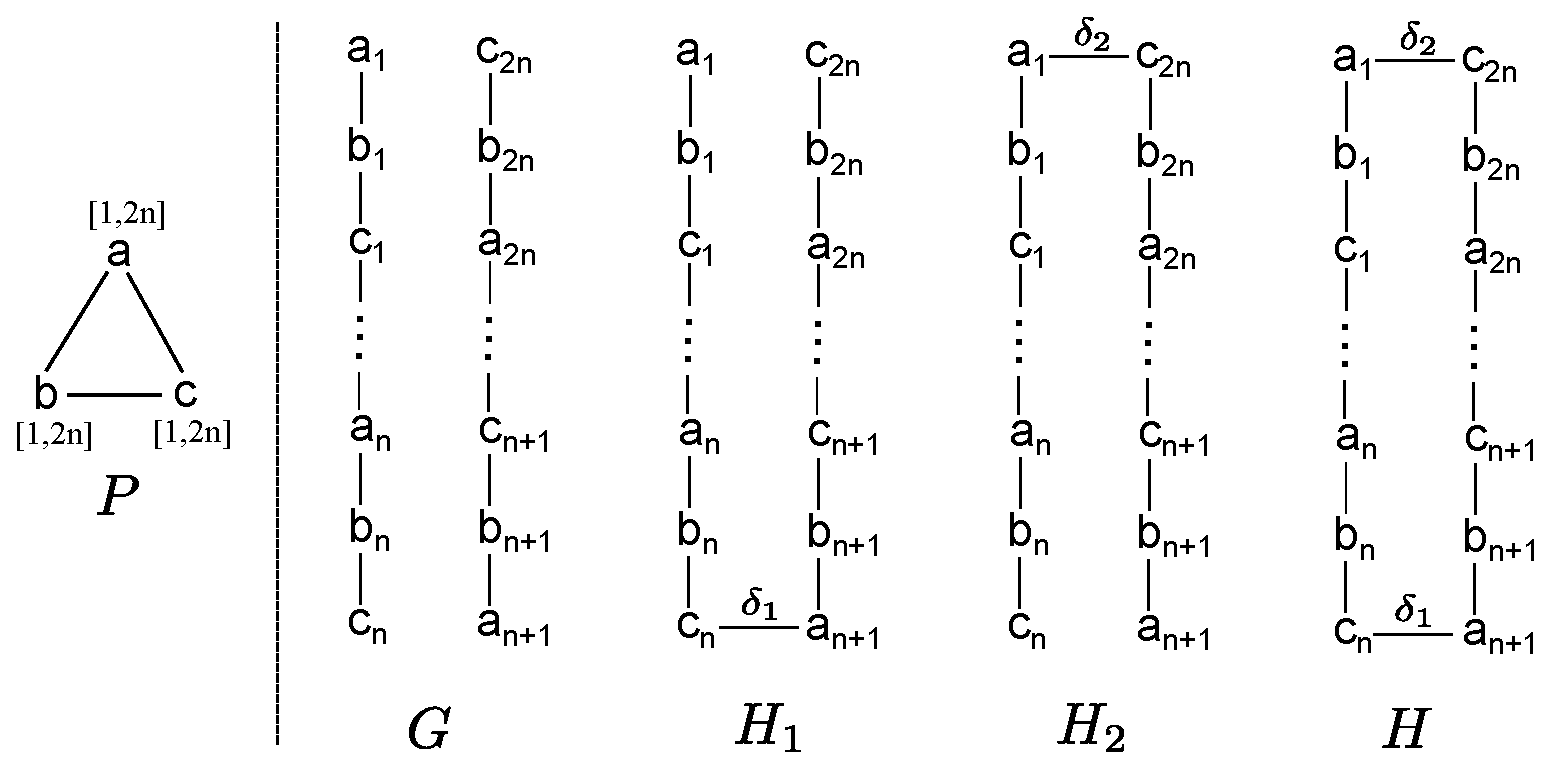
\includegraphics[scale=0.31]{./fig/inc-complexity-proof-data.eps}}
			\end{center}
			\vspace{-2.5ex}
		\end{minipage}
		\hspace{20ex}
		\begin{minipage}[t]{0.4\textwidth}
			\vspace{-0.6ex}
			\begin{center}
				\subfigure[{Unit pattern update}]{\label{fig-inc-complexity-pattern}
					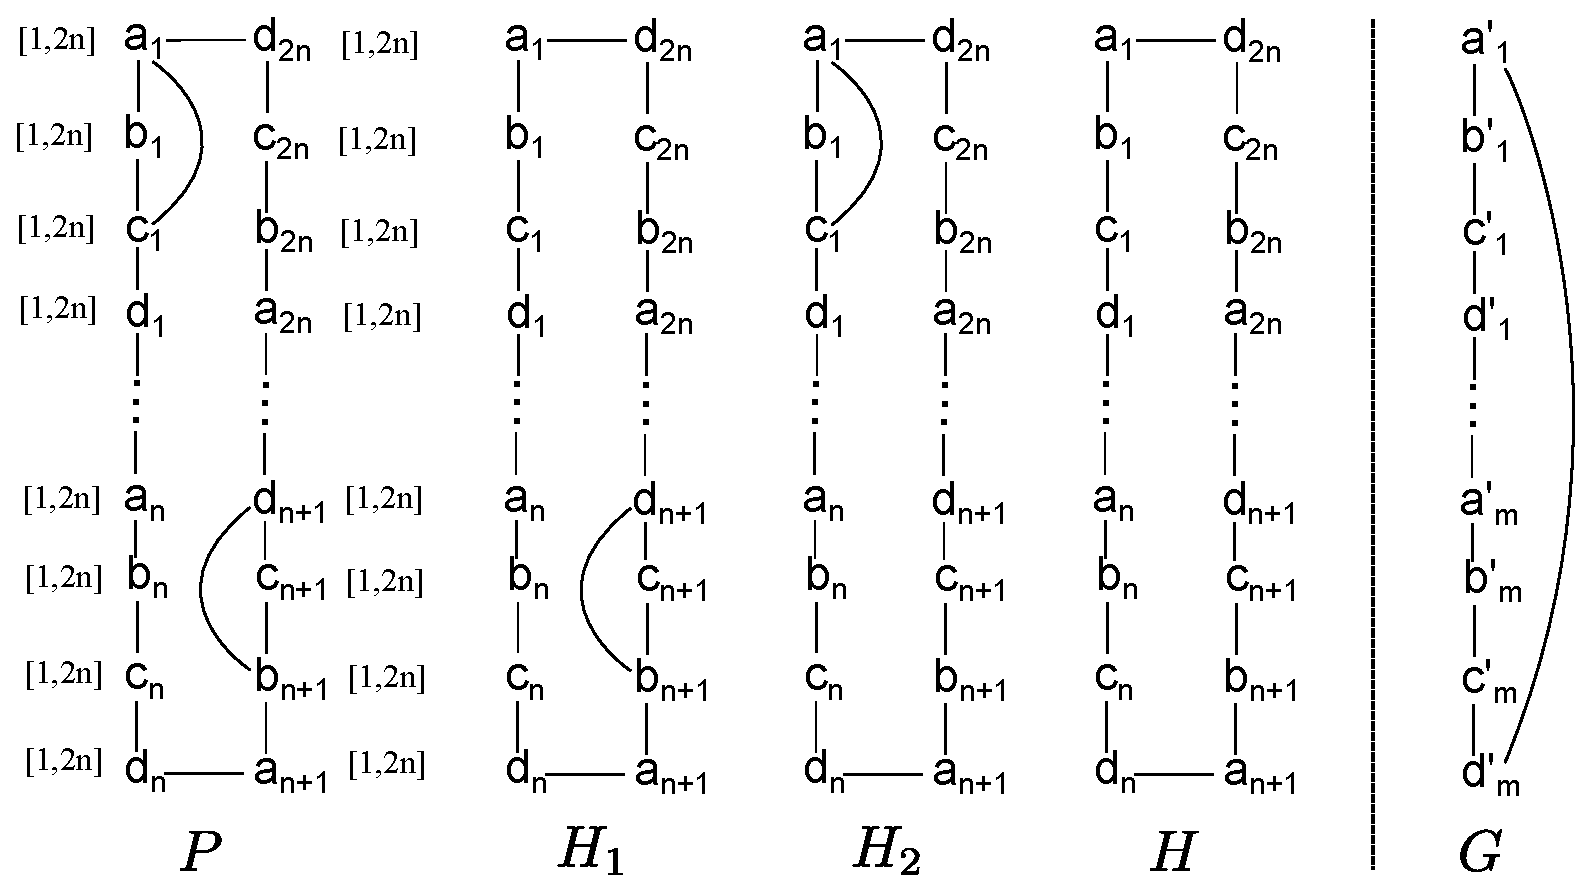
\includegraphics[scale=0.29]{./fig/inc-complexity-proof-pattern.eps}}
			\end{center}
			\vspace{-2.5ex}
		\end{minipage}
	\end{center}
	\vspace{-4ex}
	\caption{Unboundedness of unit data and pattern update}
	\label{proof-patdata-inc}
	%\end{widepage}
	\vspace{-3.0ex}
\end{figure*}

\vspace{-1.5ex}
(II) We then prove that when the algorithm outputs ``no", then pattern $P$ is unsatisfiable.
If the algorithm outputs ``no", then either (i) $P \not\eps P$ or (ii) $P \eps P$ but capacity bounds are not satisfied.
We will prove this by contradiction.
We consider case (i) $P \not\eps P$ and assume that $P$ is satisfiable.
For convenience, we use $P_1 \not\eps P_2$ to denote $P \not\eps P$, while $P_1$, $P_2$ and $P$ are exactly same.
From that $P$ is satisfiable, we know that there exists a data graph $G$ such that $P_1 \eeps G$, $P_2 \eeps G$ and $P_1 \eeps G_s$, where $G_s$ is the perfect subgraph in $G$.
By the definition of team simulation and graph simulation, from $P_2 \eeps G$, we know that $G_s \eps P_2$;
from $P_1 \eeps G_s$, we know that $P_1 \eps G_s$; and 
from $P_1 \eps G_s$ and  $G_s \eps P_2$, we know that $P_1 \eps P_2$.
This contradicts the assumption.
We then consider case (ii), $P \eps P$ \wrt $\Reps$ while there exists $(u, v)\in \Reps$ with the capacity bounds $[x_u, y_u]$ on $u$ and $[x_v, y_v]$ on $v$, respectively, and $x_v > y_u$, and assume that $P$ is satisfiable.
From $P$ is satisfiable, we know that there exists a data graph $G$ such that $P \eeps G$.
From $P \eps P$ \wrt $\Reps$ and $(u, v)\in \Reps$, we know that for any nodes $w$ in $G$, if $w$ matches the pattern node $v$, then it must match the pattern node $u$, that is, the number of data nodes match $u$ is larger than that of data nodes match $v$.
However, this contradicts that the upper bound of $u$ ($y_u$) is smaller than the lower bound of $v$ ($x_v$).
%From (I) and (II) the correctness of the algorithm follows.


\noindent
{\textbf{2. Proof of Theorem~\ref{thm-tsim-radius}}}

We will prove Theorem~\ref{thm-tsim-radius} (1) firstly.
We know that $P\eps \ball{[v, t]}$, and suppose that $M_t$ is the maximum match relation for $P$ in $\ball{[v, t]}$.
Since $\ball{[v, t]}$ is a subgraph of $\ball{[v, r]}$, 
there must exist a binary relation $M_r$ such that for any $(u, v) \in M_t$, where $u$ is a pattern node and $v$ is the matched data node of $u$ in $\ball{[v, t]}$, 
$(u, v) \in M_r$ holds, where $v$ is the matched data node of $u$ in $\ball{[v, r]}$, \ie $M_t \subset M_r$.
Since $M_t$ is the maximum match relation for $P$ in $\ball{[v, t]}$ and $M_t \subset M_r$, by the definition of graph simulation, then $P\eps \ball{[v, r]}$ and $M_r$ is a match relation for $P$ in $\ball{[v, r]}$.	

\vspace{-1ex}	
We will prove Theorem (2) using the lemma below. 

\vspace{-2.7ex}
\begin{lemma}
	\label{lemma-innerball}
	For any data graphs $G_1$ and $G_2$, and pattern graph $P$, if $G_1$ is a subgraph of $G_2$,
	then $M_1 \subset M_2$, where $M_i$ $(i=1,2)$ is the maximum match relation for $P$ in $G_i$ via graph simulation. 
\end{lemma}
\vspace{-2.5ex}

We next prove the lemma and then use the lemma to prove Theorem~\ref{thm-tsim-radius} (2).

\vspace{-1.3ex}
\stitle{Proof of Lemma~\ref{lemma-innerball}:} We will prove the lemma by contradiction. 
We know that $G_1$ is a subgraph of $G_2$, and suppose $M_1 \not\subset M_2$.
That is, there exists a pair of nodes $(u, v) \in M_1$, where $u$ is a pattern node 
and $v$ is the matched data node of $u$, but $(u, v) \not\in M_2$.
By the definition of graph simulation, from $(u, v) \in M_1$, we know that for any child node $u'$ of $u$ in $P$,
there exists a child node $v'$ of $v$ in $G_1$ such that $(u', v') \in M_1$.
From $(u, v) \not\in M_2$, we know that there exists a child node $u''$ of $u$ in $P$, 
but there exist no child nodes $v''$ of $v$ in $G_2$, such that $(u'', v'') \eps M_2$.
The process to compute maximum match relations for graph simulation is a recursive process to 
remove unmatched nodes from the initialized match relations $M$.
Because there exist no $u''$ in $G_2$ such that $(u'', v'') \eps M_2$, $(u, v)$ is removed from $M_2$.
Since $G_1$ is a subgraph of $G_2$, $(u, v)$ should also be removed from $M_1$, 
such that $(u, v) \not\in M_1$.
This contradicts the assumption that $(u, v) \in M_1$, and we get the lemma proved.
\eop

\vspace{-1.5ex}
By Lemma~\ref{lemma-innerball}, since $\ball{[v, t]}$ is a subgraph of $\ball{[v, r]}$, then $M' \subset M$.
By the definition of match graphs, since $M' \subset M$, then $G'_s$ is a subgraph of $G_s$.


\noindent
{\textbf{3. Proof of Proposition~\ref{thm-inc-grouprec-pat}}}

Incremental complexity is defined in terms of LP (locally persistent) graph algorithms \cite{Reps96}.
We also adopt the notion to prove unboundedness of graph algorithms for \dynteamF.

\vspace{-1.5ex}
The proofs below strictly follows the one in \cite{Reps96}.

%\vspace{-1.5ex}
%\begin{figure}[h]
%	\label{fig-inc-complexity-data}
%	\begin{center}
%		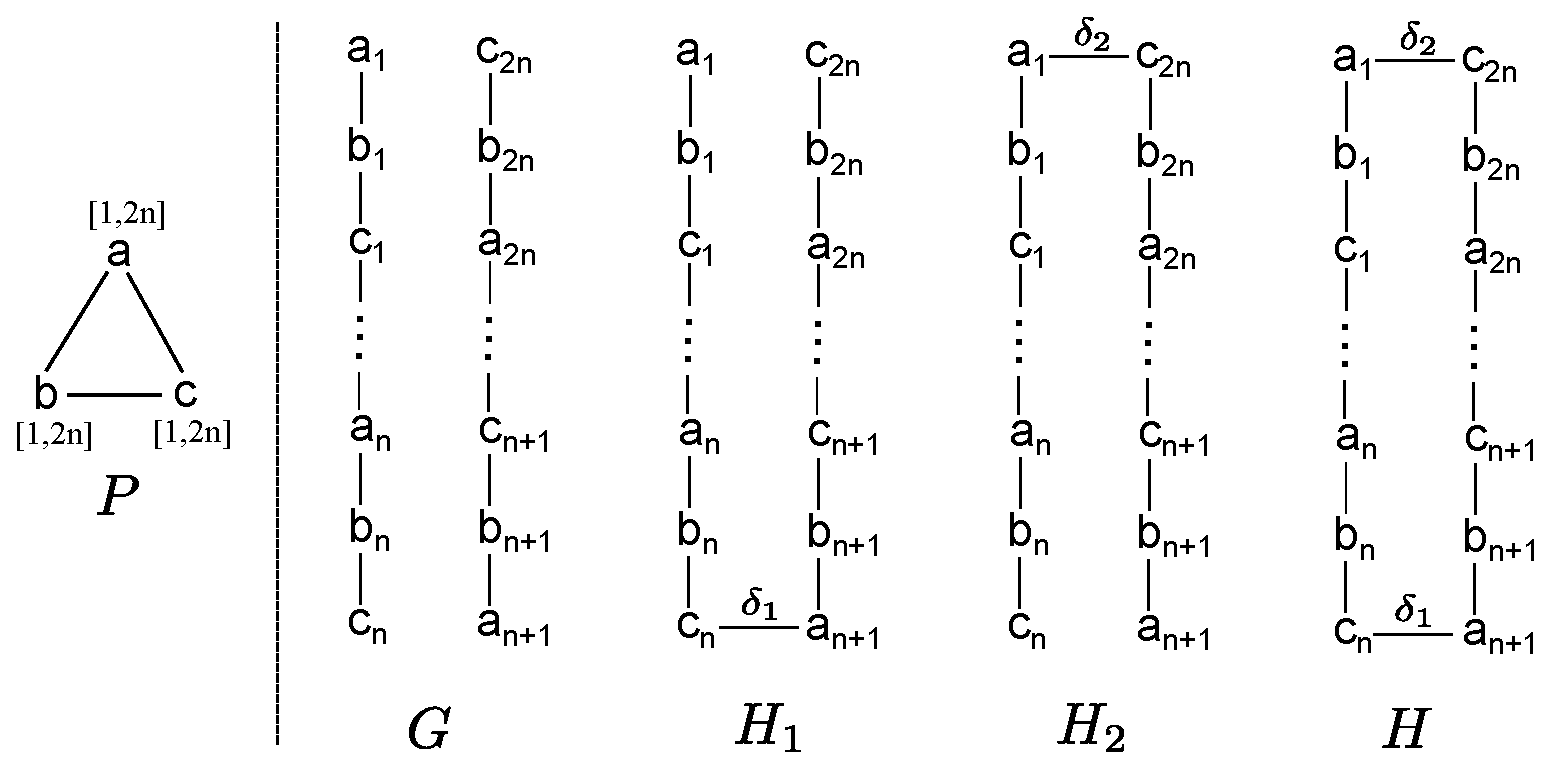
\includegraphics[scale=0.3]{./fig/inc-complexity-proof-data.eps}
%	\end{center}
%	\vspace{-3ex}
%	\caption{Unboundedness of unit data update}
%	\vspace{-2ex}
%\end{figure}

\vspace{-1.5ex}
\etitle{(I) \dynteamF\, is unbounded for unit data update}.
%Following \cite{Reps96, FanWW13-tods},
Consider the following pattern and data graph, and unit data updates, as shown in Fig.~\ref{proof-patdata-inc} (a).
Let data graph $G$ consist of two chains ($a_1$, $b_1$, $c_1$, \ldots, $a_n$, $b_n$, $c_n$) and ($a_{n+1}$, $b_{n+1}$, $c_{n+1}$, \ldots, $a_{2n}$, $b_{2n}$, $c_{2n}$) where $a_i$, $b_i$ and $c_i$ have labels $A$, $B$ and $C$ respectively.
Let pattern graph be a triangle with nodes $a$, $b$ and $c$ with labels $A$, $B$ and $C$ respectively.
Consider two unit edge insertions $\delta_1$ = $(c_n$, $a_{n+1})^+$ and $\delta_2$ = $(c_{2n}$, $a_1)^+$,
and set $k = 1$ and $r$ = $6n$.
Let $H_1$ and $H_2$ denote the graphs $G\oplus \delta_1$ and $G\oplus \delta_2$, respectively.
Obviously, $L_{k}(P, G) = L_{k}(P, H_1) = L_{k}(P, H_2) = \emptyset$,
while $L_{k}(P, H_1\oplus \delta_2) \neq \emptyset$.
Assume that there exists a locally persistent incremental algorithm ${\cal A}$ for \dynteamF.
Let $Trace(G', \delta')$ denote the sequence of steps executed by ${\cal A}$ in processing some update $\delta'$ to some graph $G'$.
Now consider the following two instances: the application of update $\delta_2$ to $G$ and the application of update $\delta_2$ to graph $H_1$.
Obviously, the update process must behave differently in these two cases, and $Trace(G, \delta_2)$ must be different from $Trace(H_1, \delta_2)$
(because many nodes of $H_1\oplus \delta_2$ are affected, while no node in $G\oplus \delta_2$ is affected).
Since a locally persistent algorithm makes no use of global storage, this can happen only both $Trace(G, \delta_2)$ and $Trace(H_1, \delta_2)$ include a visit to some node $w$ that contains different information in the graphs $G$ and $H_1$.
However, $H_1$ was obtained from $G$ by applying update $\delta_1$.
Hence the information at node $w$ must have been changed during the updating of applying $\delta_1$ to $G$.
Therefore, $Trace(G, \delta_1)$ must also contain a visit to node $w$.
As a characteristic of locally persistent algorithms is that if a node $w$ is visited during the updating of applying change $\delta'$ to graph $G'$,
then every node on some path in $G'$ from a modified node of $\delta'$ to $w$ must have been visited.
Therefore, $Trace(G, \delta_1)$ and $Trace(G, \delta_2)$ both contain a visit to $w$,
from the nodes in $\delta_1$ and $\delta_2$, respectively.
Thus, $Trace(G, \delta_1)$ and $Trace(G, \delta_2)$ include visits to every node on the path from $c_n$ or $a_{n+1}$ to $c_{2n}$ or $a_1$ respectively.
Hence, the time taken for processing update $\delta_1$ to $G$ plus the time taken for processing update $\delta_2$ to $G$ must be no smaller than the distance between $c_n$ or $a_{n+1}$ to $c_{2n}$ or $a_1$, \ie $n$, which is not a constant.
However, $|\kw{AFF}|$ in both cases are 1, such that the complexity of the incremental algorithm ${\cal A}$ cannot be measured by a function of $|\kw{AFF}|$.
Thus, ${\cal A}$ is not a bounded locally persistent incremental algorithm.
%which contradicts the assumption.

\vspace{-1.0ex}
That is, \dynteamF\, is unbounded even for $k=1$ and unit data update.
\looseness=-1

%\vspace{-1ex}
%\begin{figure}[h!]
%	\label{fig-inc-complexity-pattern}
%	\begin{center}
%		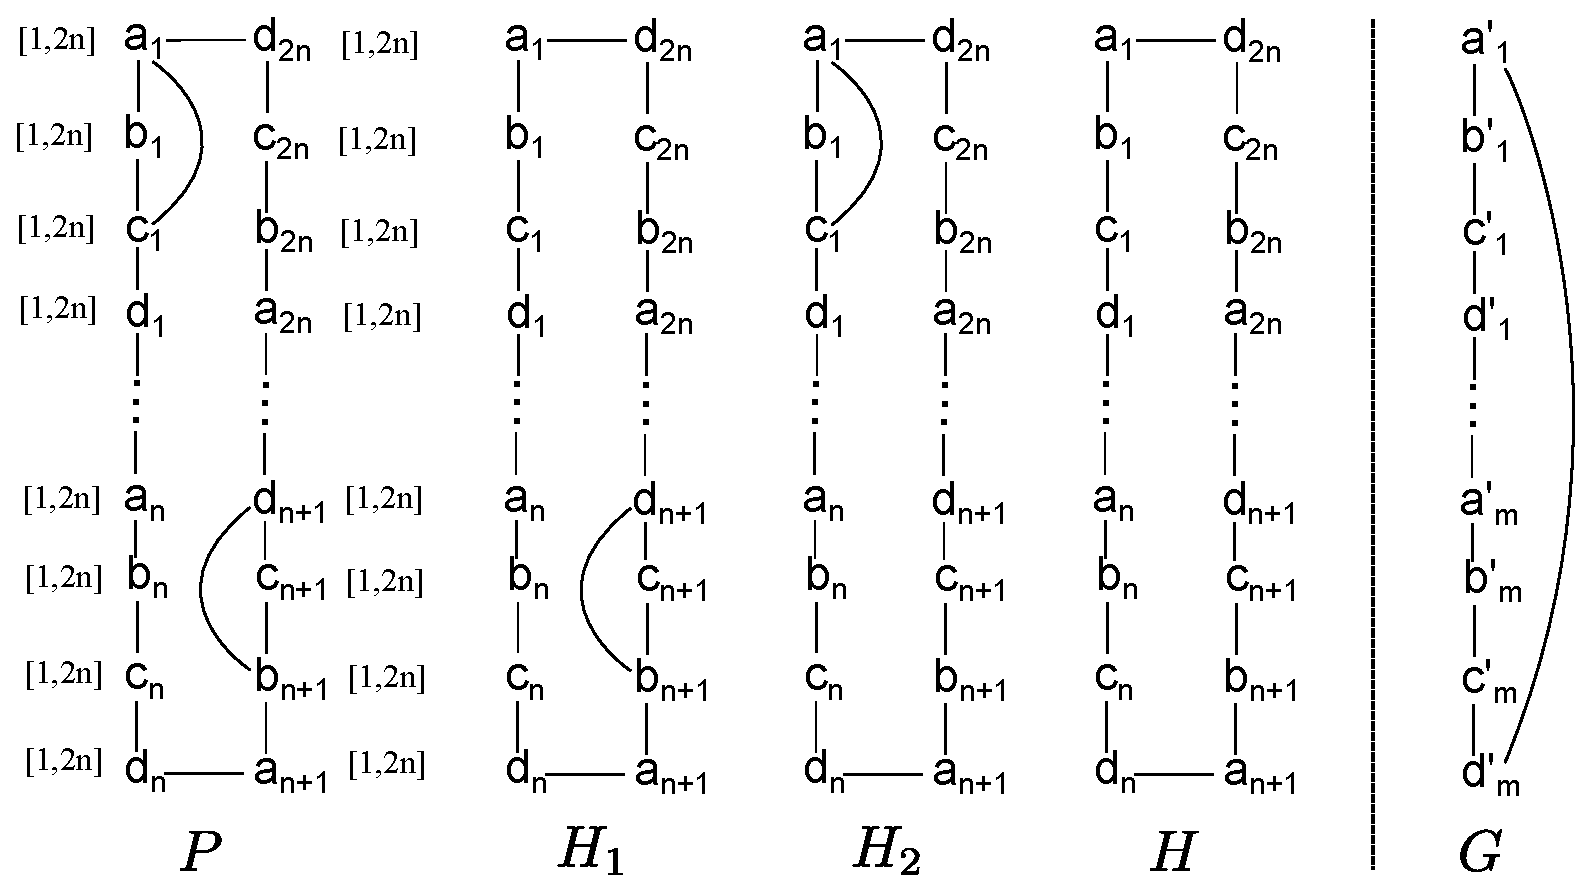
\includegraphics[scale=0.3]{./fig/inc-complexity-proof-pattern.eps}
%	\end{center}
%	\vspace{-3ex}
%	\caption{Unboundedness of unit pattern update}
%	\vspace{-2ex}
%\end{figure}

\vspace{-1.5ex}
\etitle{(II) \dynteamF\, is unbounded for unit pattern update}.
Consider the following pattern and data graph, and unit pattern updates, as shown in Fig.~\ref{proof-patdata-inc} (b).
Let data graph $G$ be a cycle ($a'_1$, $b'_1$, $c'_1$, $d'_1$, \ldots, $a'_m$, $b'_m$, $c'_m$, $d'_m$, $a'_1$),
where $a'_i$, $b'_i$, $c'_i$ and $d'_i$ have labels $A$, $B$, $C$ and $D$ respectively.
Let pattern graph be a cycle ($a_1$, $b_1$, $c_1$, $d_1$, \ldots, $a_n$, $b_n$, $c_n$, $d_n$, $a_{n+1}$, $b_{n+1}$, $c_{n+1}$, $d_{n+1}$, \ldots, $a_{2n}$, $b_{2n}$, $c_{2n}$, $d_{2n}$, $a_1$) and two extra edges ($a_1$, $c_1$) and ($b_{n+1}$, $d_{n+1}$),
where $a_i$, $b_i$, $c_i$ and $d_i$ have labels $A$, $B$, $C$ and $D$ respectively.
Consider two unit edge deletions $\delta_1$ = $(a_1$, $c_1)^-$ and $\delta_2$ = $(b_{n+1}$, $d_{n+1})^-$,
and set $k = 1$ and $r$ = $4m$.
Let $H_1$ and $H_2$ denote the graphs $P\oplus \delta_1$ and $P\oplus \delta_2$, respectively.
Obviously, $L_{k}(P, G) = L_{k}(H_1, G) = L_{k}(H_2, G) = \emptyset$,
while $L_{k}(H_1\oplus \delta_2, G) \neq \emptyset$.
Assume there exists a locally persistent incremental algorithm ${\cal A}$ for \dynteamF.
Let $Trace(P', \delta')$ denote the sequence of steps executed by ${\cal A}$ in processing some update $\delta'$ to some pattern $P'$.
Now consider two instances: the application of update $\delta_2$ to $P$ and the application of update $\delta_2$ to $H_1$.
Obviously, the update process must behave differently in these two cases, and $Trace(P, \delta_2)$ must be different from $Trace(H_1, \delta_2)$
(because many nodes in $G$ for $H_1\oplus \delta_2$ are affected, while no node in $G$ for $P\oplus \delta_2$ is affected).
Since a locally persistent algorithm makes no use of global storage,
this can happen only both $Trace(P, \delta_2)$ and $Trace(H_1, \delta_2)$ include a visit to some node $w$ that contains different information in $P$ and $H_1$.
However, $H_1$ was obtained from $P$ by applying $\delta_1$.
Hence the information at node $w$ must have been changed during the updating of applying $\delta_1$ to $P$.
Therefore, $Trace(P, \delta_1)$ must also contain a visit to node $w$.
%As a characteristic of locally persistent algorithms is that if a node $w$ is visited during the updating of applying update $\delta'$ to pattern $P'$,
%then every node in some path in $P'$ from a modified node of $\delta'$ to $w$ must have been visited.
According to the characteristics of locally persistent algorithms as illustrated in the data updates case,
$Trace(P, \delta_1)$ and $Trace(P, \delta_2)$ both contain a visit to $w$,
from the nodes in $\delta_1$ and $\delta_2$, respectively.
Thus, $Trace(P, \delta_1)$ and $Trace(P, \delta_2)$ include visits to every node on the path from $a_1$ or $c_1$ to $b_{n+1}$ or $d_{n+1}$ respectively.
Hence, the time taken for processing $\delta_1$ to $P$ plus the time taken for processing $\delta_2$ to $P$ must be no smaller than the distance between $a_1$ or $c_1$ to $b_{n+1}$ or $d_{n+1}$, \ie $4n$, which is not a constant.
However, $|\kw{AFF}|$ in both cases are 1, such that the complexity of algorithm ${\cal A}$ cannot be measured by a function of $|\kw{AFF}|$.
Thus, ${\cal A}$ is not a bounded locally persistent incremental algorithm.
%which contradicts the assumption.
That is, \dynteamF\, is unbounded even for $k=1$ and unit pattern update.

\vspace{-1.0ex}
(1) and (2) together prove that \dynteamF\, is unbounded even for $k=1$ and unit pattern or data update.


\noindent
{\textbf{4. Proof of Theorem~\ref{thm-compose}}}

We will prove the theorem by induction.
Given pattern $P(V_P,E_P)$ and its fragmentation \{${P}_{f1}$, \ldots, ${P}_{fh}$, $C$\},
we use $P^{C}(V_{P^{C}},E_{P^{C}})$ to denote the pattern with $V_{P^{C}}$=$V_P$ and $E_{P^{C}}$=$E_P/C$.
%we use $P^{C}(V_P,E_P/C)$ to denote the pattern with the same node set $V_P$ with $P$, and edges excluding the cut $C$ from $E_P$.
Graph simulation is an iterative process to remove unmatched nodes from the candidate nodes,
as illustrated in procedure \rgraphsim in Fig.~\ref{alg-rsim}.
We utilize $M_{C}^{k}$ (resp. $M_{i}^{k}$, $M^{k}$) to denote the match relation for $P^{C}$ (resp. $P_{fi}$, $P$) in $\ball{}$ in the $kth$ iteration.
By the definition of graph simulation, we have $M_{C}^{k}$ = $\bigcup_{i=1}^{h}M_{i}^{k}$.
To prove $M\subseteq\bigcup_{i=1}^{h}M_{i}$,
we next prove $M^{k}\subseteq M_{C}^{k}$ for each iteration instead.

\vspace{-1.8ex}
\sstab{(1)} For $k=0$, \ie the initialization step of graph simulation algorithm,
the algorithm computes the set of candidate matches for each pattern node.
As $P$ and $P^{C}$ have exactly the same node set, we have $M^{0}= M_{C}^{0}$.

\vspace{-1.8ex}
\sstab{(2)} For $k=n$ $(n\geq 0)$, if $M^{n}\subseteq M_{C}^{n}$ holds, we prove $M^{n+1}\subseteq M_{C}^{n+1}$ holds in the $(n+1)th$ iteration.
Suppose both $(u,w)\in M^{n}$ and $(u,w)\in M_{C}^{n}$ hold,
and in the $(n+1)th$ iteration, $(u,w)$ is removed from $M_{C}^{n}$ if there is an adjacent node $u'$ of $u$ in $P_{C}$,
but there exists no adjacent node $w'$ of $w$ in $G$ such that $(u',w')\in M_{C}^{n}$.
Therefore, $(u,w)$ must be removed from $M^{n}$ as $E_{P^{C}} \subseteq E_{P}$,
that is, the edge $(u,u')$ in $E_{P^{C}}$ must belong to $E_{P}$.
Thus, we have $M^{n+1}\subseteq M_{C}^{n+1}$.

\vspace{-1.5ex}
By (1) and (2), we have proven that $M\subseteq\bigcup_{i=1}^{h}M_{i}$.

\noindent
{\textbf{5. Proof of Proposition~\ref{prop-fragmentation}}}

The decision version of the {\em pattern fragmentation} problem, denoted by $\kw{dOFGP}(P, h, r_1, r_2)$,
is to decide whether there exists a fragmentation \{${P}_{f1}$, \ldots, $P_{fh}$, $C$\} such that,
(a) $\max_i |P_{fi}| \leq r_1\cdot\frac{|P|}{h}$ and (b) $|C|\leq r_2|P|$.

\vspace{-1.5ex}
\etitle{Upper bound.} We show the \NP upper bound by providing an \NP algorithm to determine whether there exists an $h$-fragmentation of $P$.\,Given $P$, the algorithm works as follows.
\looseness=-1

\vspace{-1.8ex}
\sstab{(1)} Guess an $h$-fragmentation ${\cal P}_h$ of $P$.

\vspace{-1.8ex}
\sstab{(2)} Check whether it satisfies restrictions of $r_1$ and $r_2$ (conditions (a) and (b) in the definition of $\kw{dOFGP}$).
If so, return yes, otherwise go to the first step and guess another instance.

\vspace{-1.5ex}
The algorithm is in \NP since step~(2) can be checked in \PTIME (liner time, indeed).

\revise{
\vspace{-1.5ex}
\etitle{Lower bound.}
We next show that it is \NP-hard to determine whether there exists an $h$-fragmentation and remains \NP-hard even when $h$ = 2,
by reduction from the {\em minimum cut} problem, which is known \NP-complete\footnote{\small http://www.nada.kth.se/$\sim$viggo/wwwcompendium/node85.html}.

\vspace{-1ex}
An instance of the minimum cut problem is given an undirected graph $H=(V_{H},E_{H})$ and a positive integer $m$,
to find a set $S \subseteq E_{H}$ of edges whose removal leaves two disjoint connected components, with $|S|\leq m$.

\vspace{-1ex}
Given an instance of the minimum cut problem,
we construct an instance of $h$-fragmentation problem.
It can be achieved by taking $H$ as $P$, and setting $h=2$, $r_1=h$ and $r_2 = m/|P|$.
Indeed, the minimum cut problem is a special case of the of $h$-fragmentation problem.}


\eat{%%%% Wrong proof %%%
\vspace{-2.5ex}
\etitle{Lower bound.}
We next show that it is \NP-hard to determine whether there exists an $h$-fragmentation and remains \NP-hard even when $h$ = 2,
by reduction from the {\em minimum cut} problem, which is known \NP-complete\footnote{\small http://www.nada.kth.se/$\sim$viggo/wwwcompendium/node85.html}.

\vspace{-2ex}
An instance of the minimum cut problem is given an undirected graph $H=(V_{H},E_{H})$ and a positive integer $m$,
to find a set $S \subseteq E_{H}$ of edges whose removal leaves two disjoint connected components, with $|S|\leq m$.

\vspace{-2ex}
Given an instance of the minimum cut problem,
we construct an instance of $h$-fragmentation problem.
It can be achieved by taking $H$ as $P$, and setting $h=2$, $r_1=h$ and $r_2 = m/|P|$.
Indeed, the minimum cut problem is a special case of the of $h$-fragmentation problem.
}%%EAT

\noindent
{\textbf{6. Proof of Proposition~\ref{prop-canaffballs}}}

The proposition is correct as when $\Delta P$ comes, the perfect subgraphs must reside in the balls that match all pattern fragments of $P\oplus \Delta P$.
\identifyaffball identifies \affballsx who already match all fragments of $P$;
Or else, if there exists a fragment $P_{fi}$ of $P$ that an \affballx cannot match,
there must exist an edge/node deletion in $\Delta P$ on $P_{fi}$,
such that the ball may match the updated fragment $P_{fi}\oplus \Delta P$.
Thus, \identifyaffball filters out the balls that cannot not match at least one fragment of $P$, and there are no deletion updates on the fragment.

\noindent
{\textbf{7. Proof of Proposition~\ref{prop-affected-datainc}}}
	
The proof is similar to the one of Proposition~\ref{prop-canaffballs}.
\identifyaffball filters out the balls that cannot match all pattern fragments,	and there are no data updates on the ball.


%%%%%%%%%%%%%%%%%%%%%%%%%%%%%%%%%%%%%%%%%%%%%%%%%
\begin{figure*}[tb!]
	%\begin{widepage}
	%\vspace{-2ex}
	\begin{center}
		%\hspace{-5.5ex}
		\subfigure[{\scriptsize Varying $|V_{P}|$ (\youtube)}]{\label{fig-exp-semantic-youtube-diameter}
			\includegraphics[scale=0.38]{./fig/youtube-semantic-diameter.eps}}
		\hspace{0.2ex}
		\subfigure[{\scriptsize Varying $|V_{P}|$ (\youtube)}]{\label{fig-exp-semantic-youtube-density}
			\includegraphics[scale=0.38]{./fig/youtube-semantic-density.eps}}
		\hspace{0.2ex}
		\subfigure[{\scriptsize Varying $|V_{P}|$ (\youtube)}]{\label{fig-exp-semantic-youtube-capacity}
			\includegraphics[scale=0.38]{./fig/youtube-semantic-capacity.eps}}
		\hspace{0.2ex}
		\subfigure[{\scriptsize Varying $|V_{P}|$ (\youtube)}]{\label{fig-exp-semantic-youtube-link}
			\includegraphics[scale=0.38]{./fig/youtube-semantic-link.eps}}
		\vspace{-2.5ex}
		
		%\hspace{-5.5ex}
		\subfigure[{\scriptsize Varying $k$ (\youtube)}]{\label{fig-exp-semantic-youtube-diameter-varyk}
			\includegraphics[scale=0.38]{./fig/youtube-semantic-diameter-varyk.eps}}
		\hspace{0.2ex}
		\subfigure[{\scriptsize Varying $k$ (\youtube)}]{\label{fig-exp-semantic-youtube-density-varyk}
			\includegraphics[scale=0.38]{./fig/youtube-semantic-density-varyk.eps}}
		\hspace{0.2ex}
		\subfigure[{\scriptsize Varying $k$ (\youtube)}]{\label{fig-exp-semantic-youtube-capacity-varyk}
			\includegraphics[scale=0.38]{./fig/youtube-semantic-capacity-varyk.eps}}
		\hspace{0.2ex}
		\subfigure[{\scriptsize Varying $k$ (\youtube)}]{\label{fig-exp-semantic-youtube-link-varyk}
			\includegraphics[scale=0.38]{./fig/youtube-semantic-link-varyk.eps}}
		\vspace{-2.0ex}
		
	\end{center}
	\vspace{-3.0ex}
	\caption{Performance evaluation of \optgrouprec for top-$k$ team formation problem}
	\label{exp-semantic-effectiveness-youtube}
	%\end{widepage}
	\vspace{-3.0ex}
\end{figure*}


%%%%%%%%%%%%%%%%%%%%%%%%%%%%%%%%%%%%%%%%%%%%%%%%%


\vspace{1ex}
\noindent
{\large \textbf{Appendix C: Detailed Correctness \& Complexity Analysis}}
\label{sec-apd-complexity}

\noindent
{\textbf{1. Algorithm \incp (Section~\ref{subsec-Qinc})}}

The correctness of \incp \wrt $\Delta P$ is assured by
the correctness of (a) \identifyaffball (by Proposition~\ref{prop-canaffballs});
(b) \incmatch, which is assured by the correctness of \rgraphsim that has been proved in Section~\ref{sec-tsimAlg}, and the correctness of of \patedgeinsert. Indeed, \patedgeinsert only removes
nodes that are no longer valid matches in each $M(P_{fi}, \ball{[v,r]})$;
(c) \comb, whose analysis follows the same way as that of \patedgeinsert; and
(d) the early return property (by Lemma~\ref{lemma-approximation-bound}).

\vspace{-1.5ex}
Procedure \identifyaffball runs in $O(2^{h}\cdot(|\Delta P|+h) +||\affballsx||)$ time, where it takes $O(2^{h}\cdot|\Delta P|)$ time to update \bfc, $O(2^{h}\cdot h)$ to do the AND-operation, and $O(||\affballsx||)$ to identify \affballsx.
%Thus, procedure \identifyaffball runs in $O(2^{h}\cdot(|\Delta P|+h) +||\affballsx||)$.
As $h$ is typically small, \eg 2 to 5, thus \identifyaffball is in $O(|\Delta P|+||\affballsx||)$;
\patedgeinsert is in $O(|M(P_{fi}, \ball{[v,r]})|+|V_{P_{fi}}||E_{\ball{[v,r]}}|)$ time.
Indeed, the recursive process for checking invalid nodes in $M(P_{fi}, \ball{[v,r]})$ is bounded by $O(|V_{P_{fi}}||E_{\ball{[v,r]}}|)$,
and the process to update $M(P_{fi}, \ball{[v,r]})$ is bounded by the size of its changes, which is monotonically decreasing;
According to \patedgeinsert,
\comb is in $O(|\bigcup^{h}_{i=1} rM(P_{fi}\oplus\Delta P_{fi},\ball{[v,r]})|+r|V_{P\oplus \Delta P}||E_{\ball{[v,r]}}|)$ time.

\vspace{-1.5ex}
Putting these together, algorithm \incp is in
$O(\bigcup_{\hat{G}\in \affballsx}\bigcup_{i\in[1,h]}(|M(P_{fi}, \hat{G})|+r|M(P_{fi} \oplus \Delta P_{fi}, \hat{G})|) + r|P \oplus \Delta P||\affballsx|$ +$|\Delta P|)$ time \wrt $\Delta P$.


\noindent
{\textbf{2. Algorithm \incd (Section~\ref{subsec-Ginc})}}

The correctness of \incd \wrt $\Delta G$ is assured by the correctness of
\identifyaffball (by Proposition~\ref{prop-affected-datainc}) and procedures \incmatch and \comb,
which can be proved along the same lines as for pattern updates.

\vspace{-1.5ex}
One can verify that \identifyaffball is in $O(|\affballsx| + |\Delta G|)$,
\incmatch for all fragments and all \affballsx is in $O(|P||\affballsx|)$ time, and \comb is in $O(\bigcup_{i\in[1,h]}r|M(P_{fi}, \widehat{G\oplus\Delta G})|$ + $r|V_{P}||E_{\widehat{G\oplus\Delta G}}|)$ time.
Therefore, algorithm \incd is in
$O(\bigcup_{\widehat{G\oplus\Delta G}\in \affballsx} \bigcup_{i\in[1,h]}r|M(P_{fi}, \widehat{G\oplus\Delta G})|+r|P||\affballsx| + |\Delta G|)$ time \wrt $\Delta G$.

\vspace{1ex}
\noindent
{\large \textbf{Appendix D: Extra Experiments}}
\label{sec-apd-exp}

\vspace{-0.5ex}
The experimental results on \youtube are reported here.

\vspace{-1.8ex}
\stitle{Exp-1: Performance of \optgrouprec}. We firstly evaluated the performance of \optgrouprec vs. \mindia, \minsumdis and \denalk on \youtube \wrt four quality measures.
The results are reported in Fig.~\ref{fig-exp-semantic-youtube-diameter} to~\ref{fig-exp-semantic-youtube-link-varyk}.
We find \optgrouprec strikes a balance at capturing the practical requirements.

\vspace{-1.8ex}
\stitle{Exp-2: Efficiency of \inc for one set of updates}. Varying the amount of updates in one update set from 4.5\% to 49.5\% for pattern updates, 2.5\% to 27.5\% (resp. 3\% to 33\%) for data insertions and hybrid data updates (resp. data deletions), and (4.5\%, 2.5\%) to (31.5\%, 17.5\%) for simultaneous pattern and data updates, the results are reported in Fig.~\ref{fig-exp-patinc-del-youtube} to~\ref{fig-exp-hyb-patdata-youtube}.
We find that \inc outperforms \optgrouprec when $\Delta P$, $\Delta G$ and $(\Delta P$, $\Delta G)$ are no more than 36\%, 22.5\% and (27\%, 15\%).
%for hybrid pattern, hybrid data, and simultaneous pattern and data updates.

\vspace{-1.8ex}
\stitle{Exp-3: Efficiency of \inc for continuous sets of updates}. We generated 5 sets of updates,
varying the amount of updates from 4.5\% to 27\% for pattern updates, 2.5\% to 15\% for data updates,
and (4.5\%, 2.5\%) to (22.5\%, 12.5\%) for simultaneous pattern and data updates.
We evaluated the average time took by \inc to process these sets of updates one by one.
The results are reported in Fig.~\ref{fig-exp-patinc-multi-youtube} to~\ref{fig-exp-hyb-datapat-multi-youtube}.
We find \inc outperforms \optgrouprec when changes are no more than 27\%, 10\% and (13.5\%, 7.5\%) for continuous pattern, data and simultaneous updates respectively.

\vspace{-1.8ex}
\stitle{Exp-4: Physical storage of auxiliary structures}. As shown in Fig.~\ref{fig-exp-youtube-extraspace},
it takes 58MB extra space to store all auxiliary structures utilized by \inc on \youtube, which need 114MB space to store itself,
\ie 50.8\% compared with the original dataset.

\begin{figure*}[t!]
	%\begin{widepage}
	%\vspace{-1.5ex}
	\begin{center}
		%\hspace{-5.5ex}
		\subfigure[{\scriptsize Varying $|\Delta P|$ (deletions)}]{\label{fig-exp-patinc-del-youtube}
			\includegraphics[scale=0.38]{./fig/youtube-pattern-deletion.eps}}
		\hspace{0.2ex}
		\subfigure[{\scriptsize Varying $|\Delta P|$ (insertions)}]{\label{fig-exp-patinc-ins-youtube}
			\includegraphics[scale=0.38]{./fig/youtube-pattern-insertion.eps}}
		\hspace{0.2ex}
		\subfigure[{\scriptsize Varying $|\Delta P|$ (capacity)}]{\label{fig-exp-patinc-cap-youtube}
			\includegraphics[scale=0.38]{./fig/youtube-pattern-capchange.eps}}
		\hspace{0.2ex}
		\subfigure[{\scriptsize Varying $|\Delta P|$ (hybrid updates)\hspace{-8.5ex}}]{\label{fig-exp-patinc-hyb-youtube}
			\includegraphics[scale=0.38]{./fig/youtube-pattern-hybrid.eps}}
		\vspace{-2.5ex}
		
		%\hspace{-5.5ex}
		\subfigure[{\scriptsize Varying $|\Delta G|$ (deletions)}]{\label{fig-exp-datainc-del-youtube}
			\includegraphics[scale=0.38]{./fig/youtube-data-deletion.eps}}
		\hspace{0.2ex}
		\subfigure[{\scriptsize Varying $|\Delta G|$ (insertions)}]{\label{fig-exp-datainc-ins-youtube}
			\includegraphics[scale=0.38]{./fig/youtube-data-insertion.eps}}
		\hspace{0.2ex}
		\subfigure[{\scriptsize Varying $|\Delta G|$ (hybrid updates)}\hspace{-5.5ex}]{\label{fig-exp-datainc-hyb-youtube}
			\includegraphics[scale=0.38]{./fig/youtube-data-hybrid.eps}}
		\hspace{0.2ex}
		\subfigure[{\scriptsize Vary $(|\Delta P|,|\Delta G|)$ (simultaneous)}\hspace{-8.5ex}]{\label{fig-exp-hyb-patdata-youtube}
			\includegraphics[scale=0.38]{./fig/youtube-pattern-data.eps}}
		\vspace{-2.5ex}
		
		%\hspace{-5.5ex}
		\subfigure[{\scriptsize Varying $|\Delta P|$ in update sets}]{\label{fig-exp-patinc-multi-youtube}
			\includegraphics[scale=0.38]{./fig/youtube-pattern-multi.eps}}
		\hspace{0.2ex}
		\subfigure[{\scriptsize Varying $|\Delta G|$ in update sets}]{\label{fig-exp-datainc-multi-youtube}
			\includegraphics[scale=0.38]{./fig/youtube-data-multi.eps}}
		\hspace{0.2ex}
		\subfigure[{\scriptsize Vary $(|\Delta P|,|\Delta G|)$ in update sets}\hspace{-8.5ex}]{\label{fig-exp-hyb-datapat-multi-youtube}
			\includegraphics[scale=0.38]{./fig/youtube-pattern-data-multi.eps}}
		\hspace{0.2ex}
		\subfigure[{\scriptsize Storage sizes}]{\label{fig-exp-youtube-extraspace}
			\includegraphics[scale=0.38]{./fig/youtube-space.eps}}
		\vspace{-2ex}
		
	\end{center}
	\vspace{-3.0ex}
	\caption{Performance evaluation of \inc for dynamic top-$k$ team formation problem (\youtube)}
	\label{exp-inc-youtube}
	%\end{widepage}
	\vspace{-3.0ex}
\end{figure*}

%\newpage
%%\newcommand{\EQ}{\kw{EQ}}
\newpage
\addtolength{\parskip}{0.25cm}
\newpage
\section*{\Large \sf APPENDIX-cp}
\label{sec-proofs}



\subsection{Optimization Techniques for Algorithm \grouprec}.
%
\begin{figure}[tb!]
\vspace{2ex}
\begin{center}
{\small

\myhrule \vspace{-2ex}
\mat{0ex}{
\sstab {\sl Input:\/} Pattern graph $P(V_p$, $E_p$, $l_p$, $f_p)$.\\
{\sl Output:\/} A minimum equivalent pattern graph $P_m$ of $P$.\\
\bcc \quad if $P$ is not a consistent pattern graph then return null.\\
\icc \quad Compute the maximum match relation $S$ of $P \eps P$;\\
\icc \quad Compute equivalent classes of nodes in $P$ based on $S$;\\
\icc \quad Create a node for each equivalent class in $P_m$;\\
\icc \quad Connect different equivalent classes by necessary edges in $P_m$;\\
\icc \quad Compute the intersection of interval bounds on pattern nodes in \\each equivalent class and put on the corresponding node in $P_m$;\\
\icc return $P_m$;\\
}
\vspace{-2.5ex}

\myhrule
}
\end{center}
\vspace{-4ex}
\caption{minP} \label{minP-alg}
\vspace{-3ex}
\end{figure}

%
We next present optimization techniques for algorithm \grouprec, by means of query minimization, as stated below, yielding the optimization algorithm \grouprecopt.

Query minimization is important for any query language. Minimizing pattern graphs is an effective way for improving the efficiency of querying data graphs. By Proposition~\ref{prop-pattern-consistency}, a pattern graph can be determined whether is satisfiable or not in quadratic time. Once we know a pattern graph is consistent, the $r$-simulation computing process can be optimized by minimizing the pattern graphs.

We say two pattern graphs $P$ and $P'$ are {\em equivalent via $r$-simulation}, denoted by $P\equiv P'$, iff for any data graph $G$, $P(G) = P'(G)$ via $r$-simulation. We say $P$ is {\em minimum} if for any other pattern graph $P'$ such that $P\equiv P'$, $|P|\leq |P'|$.

\eat{
\begin{theorem}
\label{thm-pattern-minimization-ap}
For any pattern graph $P$ and radius $r$, (1) there exists a unique minimum equivalent pattern graph $P_m$, via $r$-simulation with, that finds the same maximum match relation on any data graph; (2) taking the intersection of interval bounds on pattern nodes in each equivalent class in $P_m$, and putting it on the corresponding pattern node in $P_m$, $P$ and $P_m$ are equivalent via $r$-simulation; and (3) there exists a quadratic time algorithm to find its minimum equivalent pattern graph.
\end{theorem}
}

\begin{theorem}
\label{thm-pattern-minimization-ap}
For any pattern graph $P(V_p, E_p)$ and radius $r$, (1) there exists a unique minimum equivalent pattern graph $P_m$ via $r$-simulation;
and (2) there exists an algorithm that finds $P_m$ in $((|V_p|+|E_p|)^2)$ time.
\end{theorem}


\eat{
\stitle{Remarks}.
(1) A pattern graph $P$ may have multiple minimum equivalent pattern graphs $P_m^1$, $P_m^2$,..., $P_m^k$, of the same size but are not isomorphic to each other. Their structures must be exactly same, while the capacity on the corresponding nodes may be different, but they still return the same match result on any data graph.
%
(2) There exists method to get a unique minimum equivalent pattern graph, which takes linear time. Is unifying step necessary? Adopt or not?
}

\etitle{Algorithm \minp} As a proof of Theorem~\ref{thm-pattern-minimization}, we present Algorithm \minp to minimize pattern graphs as shown in Fig.~\ref{minP-alg}. It takes as input a pattern graph $P$, and outputs a minimum equivalent pattern graph $P_m$ of $P$ via graph simulation and some capacity bound computing. For any pattern graph $P$, it first checks to see whether $P$ is consistent. If the answer is yes, it then executes the following minimization steps. In the minimization process, It first computes the maximum match relation $R$ by treating $P$ as both a pattern and a data graph(line 2). It then computes equivalent classes for nodes in $P$ such that $u$ and $v$ are in the same class iff both $(u, v)\in R$ and $(v, u)\in R$ (line 3). Finally, it constructs the minimum equivalent pattern graph $P_m$ as follows (lines 4-6).(a) For each equivalent class \kw{eq}, it creates a node \kw{eq} for $P_m$; (b) there is an edge (\kw{eq}, \kw{eq'}) in $P_m$ iff there exist nodes $u \in \kw{eq}$ and $u' \in \kw{eq'}$ such that there is an edge $(u, u')$ in $P_m$; and (c) it computes the intersection of capacity bounds on pattern nodes in each equivalent class \kw{eq} and put on the corresponding node \kw{eq} in $P_m$.


\eat{%%%%%%%%%%%EAT
\begin{figure}[tb!]
\vspace{-2ex}
\begin{center}
{\small

\myhrule \vspace{-2ex}
\mat{0ex}{
\sstab {\sl Input:\/} Pattern graph $P(V_p$, $E_p$, $l_p$, $f_p)$.\\
{\sl Output:\/} A minimum equivalent pattern graph $P_m$ of $P$.\\
\bcc \quad if $P$ is not a consistent pattern graph then return null.\\
\icc \quad Compute the maximum match relation $R$ of $P \eps P$;\\
\icc \quad Compute equivalent classes of nodes in $P$ based on $R$;\\
\icc \quad Create a node for each equivalent class in $P_m$;\\
\icc \quad Connect different equivalent classes by necessary edges in $P_m$;\\
\icc \quad Compute the intersection of interval bounds on pattern nodes in \\each equivalent class and put on the corresponding node in $P_m$;\\
\icc return $P_m$;\\
}
\vspace{-2.5ex}

\myhrule
}
\end{center}
\vspace{-4ex}
\caption{\minp} \label{minP-alg}
\vspace{-3ex}
\end{figure}
}%%%%%%%%%%%%%EAT

\begin{example}
Takes as input the pattern graph $P_3$ given in Fig.~\ref{fig-consistency-example}. Algorithm works as follows. By Proposition~\ref{prop-pattern-consistency}, it determines that $P_3$ is a consistent pattern graph. In the minimization process, it first computes the maximum match relation $S$ by taking $P_3$ as both pattern and data graph, producing $S$ = \{$(A, A)$, $(B_1, B_2)$, $(B_2, B_1)$, $(C_i, C_j)$\} ($i,j \in [1,3]$). It then computes three equivalent classes: $\kw{eq_A}$=\{$A$\}, $\kw{eq_B}$=\{$B_1, B_2$\}, and $\kw{eq_C}$=\{$C_1, C_2, C_3$\}. Finally, it constructs the minimum equivalent pattern graph $P_m$ of $P$, as shown in Fig.~\ref{fig-consistency-example}. (a) For each equivalent class $\kw{eq_A}$, $\kw{eq_B}$ and $\kw{eq_C}$, it creates node labeled with $A$, $B$, and $C$ respectively; (b) it creates an edge $(A,B)$ connecting the class nodes of $\kw{eq_A}$ and $\kw{eq_B}$ in $P_m$, as there exists an edge $(u,v)$ in $P_3$ with $u \in \kw{eq_A}$ and $v \in \kw{eq_B}$, the same for edge $(B,C)$; and (c) for equivalent class $eq_B$, it computes the intersection of interval bounds on pattern nodes in it, that is, $[1,3]\cap[2,5] = [2,3]$, and [1,1], [3,4] for $eq_A$, $eq_C$. At last it puts them on the corresponding nodes in $P_{3m}$.
\end{example}

\etitle{Correctness and Complexity}. The correctness of Algorithm \minp is assured by the following. (1) $P_m \equiv P$, ensuring they return exactly the same result on any data graph; and (2) $P_m$ is minimum in size, \ie there is no other equivalent query $P'$ smaller than $P_m$.

Algorithm minP is in $O((|V_p|+|E_p|)^2)$ time. Indeed, step 1 (line 2), 2 (line 3), 3 (line 4-5) and 4 (line 6) of minP take $O((|V_p|+|E_p|)^2)$ time, $O(|V_p|^2)$ time, $O(|E_p|)$ time and $O(|V_p|^2)$ time, respectively.

Besides, algorithm \grouprecopt builds balls only using the set of data nodes with labels included in pattern nodes, instead of using all data nodes, which is an effective improvement for algorithm \grouprec.

\eat{
\stitle{Algorithm $\incgrpat^+$}

\begin{figure}[hb!]
\vspace{-2ex}
\begin{center}
{\small

\myhrule \vspace{-2ex}
\mat{0ex}{
\sstab {\sl Input:\/} Pattern graph $Pt_i(V_{Pt_i}$, $E_{Pt_i})$, data ball $\ball{w,r}$, $mat_i(\cdot)$,\\ and an edge $e=(u,u')$ to be inserted into $Pt_i$.\\
{\sl Output:\/} The updated match relation $mat_i(\cdot)$.\\
\bcc \quad $AFNode:=\emptyset$;\\
\icc \quad for each node $v \in mat_i(u)$ do\\
\icc \quad\quad if there is no $v' \in mat_i(u')$ with $(v, v')\in V_{\hat{G}}$\\
\icc \quad\quad then $AFNode:=AFNode \cup \{v\}$;\\
\icc \quad for each node $v' \in mat_i(u')$ do\\
\icc \quad\quad if there is no $v \in mat_i(u)$ with $(v', v)\in V_{\hat{G}}$\\
\icc \quad\quad then $AFNode:=AFNode \cup \{v'\}$;\\
\icc \quad for each node $v \in AFNode$ do\\
\icc \quad\quad $wSet:=\emptyset$;\\
\icc \quad\quad for each adjacent edge $(v,v')$ of $v$ do\\
\icc \quad\quad\quad for all $(u,u')\in E_p$ having $v \in mat_i(u)$ and $v'\in mat_i(u')$ do\\
\icc \quad\quad\quad\quad if $adjacent(l_p(u),v')\cap mat_i(u)=\emptyset$ then\\
\icc \quad\quad\quad\quad\quad $wSet$.push($(u',v')$);\\
\icc \quad\quad\quad\quad\quad while ($wSet\neq \emptyset$) do\\
\icc \quad\quad\quad\quad\quad\quad $(u',v'):=wSet$.pop();\\
\icc \quad\quad\quad\quad\quad\quad $mat_i(u')=mat_i(u')\backslash\{v'\}$;\\
\icc \quad\quad\quad\quad\quad\quad for all $(u',u'')\in E_p$ do\\
\icc \quad\quad\quad\quad\quad\quad\quad for all $v''\in adjacent(l_p(u''),v')\cap mat_i(u'')$ do\\
\icc \quad\quad\quad\quad\quad\quad\quad\quad if $adjacent(l_p(u'),v'')\cap mat_i(u')=\emptyset$ then \\
\icc \quad\quad\quad\quad\quad\quad\quad\quad\quad $wSet$.push($(u'',v'')$);\\
\icc if there is a pattern node $u$ having $|mat_i(u)| = 0$ then $mat_i=\emptyset$\\
\icc return $mat_i(\cdot)$;
}

\vspace{-2.5ex} \myhrule
}
\end{center}
\vspace{-4ex}
\caption{$\incgrpat^+$} \label{incpat-unit-insert}
\vspace{-3ex}
\end{figure}
}



\stitle{Linear $2$-approximation for density upper bounding}.
Given a ball $\ball{v,r}$ in $G$ and a pattern $P$, it computes density bound $ub$ to the perfect graph $\hat{G}_s$ of $P$ in $\ball{v,r}$ in $O(|\ball{v,r}|)$ time, such that $\kw{den}(\hat{G}_s) \leq d_{\kw{max}} \leq ub$, where $\kw{den}(\hat{G}_s)$ is the density of $\hat{G}_s$ and $d_{\kw{max}}$ is the density of the densest subgraph of $\ball{v,r}$.
Therefore, we can treat $ub$ as an upper bound on the density of $\hat{G}_s$. More specifically, it computes the $ub$ in three steps, as follows.

\sstab (1) Filter out to get a subgraph $\hat{G}_P$ from ball $\ball{v,r}$ such that $\hat{G}_P$ contains nodes with labels appeared in $P$ only, and the induced edges, in $O(|\ball{v,r}|)$ time.

\sstab (2) Compute the density $d$ of the {\em maximum core} of $\hat{G}_P$ in $O(|\hat{G}_P|)$ time.

\sstab (3) Return $2d$ as the density upper bound for $\hat{G}_s$ in $\ball{v,r}$.

Here the maximum core of a graph $G$ is defined as follows~\cite{EVMK12}.
A $l$-core of a graph $G$ is a subgraph $G_l$ of $G$ such that, each node in $G_l$ has degree no smaller than $l$.
A maximum core of a graph $G$ is a $l$-core $G_l$ of $G$ such that, for any non-empty $l'$-core $G_{l'}$ of $G$, $l'\leq l$. It is known that the maximum core of a graph $G$ can be computed in $O(|G|)$ time.

The following result ensures the above linear time algorithm returns $ub$ with the property claim above.

\begin{prop}
\label{prop-approximation-bound}
Given a graph $G$, let $d$ be the density of the maximum core of $G$, and $d_{\kw{max}}$ is the density of the densest subgraph of $G$, then $d\leq d_{\kw{max}} \leq 2d$.
\end{prop}



\subsection{NP-hardness}

We first formulate the {\em optimal $m$-fragmentation problem} ($\kw{OFGP}(P,m)$) as a bi-criteria optimization problem as follows.
\bi
\item Input: pattern graph $P$, an integer $m$.
\item Output: an $m$-fragmentation ${\cal P}_{m}$ composed of ${Pf}_1$, \ldots, ${Pf}_m$ and $F$ of $P$ such that (a) $\max_i |{Pf}_i|$ = $\max_i (|V_{{Pf}_i}| + |E_{{Pf}_i}|)$ is minimized; and (b) $|F|$ is minimized.
\ei
%Here $w(u)$ (resp. $w(e)$) is to represent the probability that a pattern update was applied to node $u$ (resp. edge $e$) in, \eg history pattern update workload, and can be set to 1 if no historical information is known.
That is, the problem is to implement the ``divide and conquer'' incremental strategy of the framework by finding a good $m$-fragmentation ${Pf}_1$, \ldots, ${Pf}_m$ and $F$ of the pattern graph such that
(i) the chances of the fragments ${Pf}_i$ to be updated are roughly the same, which further guarantees that the update time on any pattern fragment ${Pf}_i$ will be roughly equal, and the update time in all fragments is also minimized; and
(ii) the size of $F$ is also minimized such that the combination cost is minimized.

The decision version of $\kw{OFGP}(P, m)$, denoted by $\kw{dOFGP}(P, m, r_1, r_2)$, is to decide whether there exists a fragmentation ${Pf}_1$, \ldots, ${Pf}_m$ and $F$ such that, (a) $\max_i |{Pf}_i| \leq r_1\cdot\frac{|P|}{m}$ and (b) $|F|\leq r_2|P|$.
The corresponding single-criteria {\em cut}-minimization (resp. {\em fragment}-minimization) problem of $\kw{OFGP}(P, m)$, denoted by $\kw{OFFGP}(P, m, r)$ (resp. $\kw{OPFGP}(P, m, r)$), is to find an $m$-fragmentation ${Pf}_1$, \ldots, ${Pf}_m$ and $F$ such that $\max_i |{Pf}_i| \leq r\cdot\frac{|P|}{m}$ (resp. $|F|\leq r\cdot |P|$) and $|F|$ (resp. $\max_i |{Pf}_i|$) is minimized.

The problems are hard, as shown below.

\begin{prop}
\label{thm-fragmentation-hardness}
(1) $\kw{dOFGP}(P, m, r_1, r_2)$ is \NP-complete. It remains \NP-hard even $m$ = 2.

\sstab (2) Both $\kw{OFFGP}(P, m, r)$ and $\kw{OPFGP}(P, m, r)$ are \NPO-hard.
\end{prop}

Here \NPO is the class of all \NP optimization problems. An
\NPO-complete problem is \NP-hard to optimize, and is among the
hardest \NP optimization problems.

\begin{proofS}
(1) We show $\kw{dOFGP}$ is in \NP by giving an \NP algorithm that first guesses an $m$-cut $F$, and then check whether it divides $P$ into an $m$-fragmentation ${Pf}_1$, \ldots, ${Pf}_m$ such that $\max_i |{Pf}_i| \leq r_1\frac{|P|}{m}$ and $|F|\leq r_2|P|$. We show it is \NP-hard by reduction from the {\sc Minimum Bisection} problem, which is known \NP-hard even when $k=2$.
(2) We shown both $\kw{OFFGP}(P, m, r)$ and $\kw{OPFGP}(P, m, r)$ are \NPO-hard by proving that it is \NP-hard to decide whether there exists a feasible solution to both of them ({\bf To be verified}).
Indeed, there is no polynomial time approximation algorithm can guarantee a finite approximation ratio for $\kw{OFFGP}(P,m,r=1)$~\cite{AndreevR06}.
\end{proofS}


In light of Theorem~\ref{thm-fragmentation-hardness}, we give a heuristic algorithm, denoted by \kw{PFrag} and shown in Fig.~\ref{alg-PFrag}, for $\kw{OFGP}(P,m)$.
Algorithm \kw{PFrag} works by connecting $\kw{OFGP}(P,m)$ to the {\sc $(k, \nu)$-Balanced Partition} problem, which is to divided the vertices of a graph into $k$ components such that each component is of size more than $\nu\cdot\frac{n}{k}$, so that the number of edges between different compopents is minimized. The $(k,\nu)$-balanced partition problem, though is not approximable in general, has a number of sophisticated heuristic algorithms~\cite{AndreevR06}.

%%%%%%%%%%%%%%%%%%%%%Algorithm PFrag
\begin{figure}[t]
\begin{center}
{\small
\begin{center}
\myhrule \vspace{-2ex}
\mat{0ex}{
\sstab {\sl Input:\/} \= Pattern graph $P$, integer $m$.\\
{\sl Output:\/} An $m$-fragmentation ${Pf}_1$, \ldots, ${Pf}_m$, $F$ of $P$.\\
\stab \bcc \hspace{0.5ex} \= $k$ = $m$; $\nu$ = $m$; $M_P$ = $|P|$; $M_F$ = 0;\\
\icc \> $({Pf}^\nu_1, \ldots, {Pf}^\nu_m, F^\nu)$ := $\kw{BalanceP}(k,\nu)$; \\
\icc \> $M^\nu_P$ := $\kw{max}\{|{Pf}^\nu_1|, \ldots, |{Pf}^\nu_m|\}$; $M^\nu_F$ = $|F^\nu|$;\\
\icc\> \While $\kw{max}\{M_P, M_F\} > \kw{max}\{M^\nu_P, M^\nu_F\}$ \Do\\
\icc \>\hspace{2ex}\= ${Pf}_1$ := ${Pf}^\nu_1$, \ldots, ${Pf}_m$ := ${Pf}^\nu_m$;\\
\icc \>\hspace{2ex}\= $F$ := $F^\nu$; $M_P$ := $M^\nu_P$; $M_F$ := $M^\nu_F$;\\
\icc \>\> \If $M^\nu_P \geq M^\nu_F$ \Then $\nu := \frac{\nu}{2}$ \Else $\nu := \frac{3\nu}{2}$;\\
\icc \>\> $({Pf}^\nu_1, \ldots, {Pf}^\nu_m, F)$ := $\kw{BalanceP}(k,\nu)$;\\
\icc \>\> $M^\nu_P$ := $\kw{max}\{|{Pf}^\nu_1|, \ldots, |{Pf}^\nu_m|\}$; $M^\nu_F$ = $|F^\nu|$;\\
\icc \> \Return ${Pf}_1$, \ldots, ${Pf}_m$, $F$;
}
\vspace{-2.5ex} \myhrule
\end{center}
}
\end{center}
\vspace{-4ex}
\caption{Algorithm \kw{PFrag} \label{alg-PFrag}}
\vspace{-3ex}
\end{figure}


Given a pattern $P$ and an integer $m$, algorithm \kw{PFrag} finds an $m$-fragmentation for $P$ by recursively invoking algorithm $\kw{BalanceP}(k,\nu)$ for the {\sc $(k,\nu)$-Balanced partition} problem with different $\nu$, such that the final returned $m$-fragmentation strikes a balance between the size of each fragment ${Pf}_i$ of $P$ and the size of the cut $F$.
More specifically, \kw{PFrag} maintains $M_P$ and $M_F$ as the size of the maximum fragment of ${Pf}_i$  and the size of the cut in the $m$-fragmentation, respectively. Initially, it sets $M_p$ to $|P|$ and $M_F$ to 0 (line~1).
It then invokes \kw{BalanceP} with both $k$ and $\nu$ being $m$, \ie has no constraints on the size of fragments of $P$ (line~2).
After that, it iteratively checks whether the generated $m$-fragmentation can be improved (line~4) by adjusting $m$ in a {\em binary search style} (lines~4-9). If the current size of maximum fragment $M^\nu_P$ is no smaller than the size $M^\nu_F$ of the cut, it invokes \kw{BalanceP} with $m$ and $\frac{\nu}{2}$, and with $m$ and $\frac{3\nu}{2}$ otherwise (line~7). It returns the $m$-fragmentation if it cannot be improved anymore in this way (line~10).

\stitle{Correctness \& Complexity}.
The correctness is obvious as \kw{PFrag} always returns $m$-fragmentations.
Algorithm~\kw{PFrag} runs in $O(\log m\cdot t_{\kw{BalanceP}})$ time, where $t_{\kw{BalanceP}}$ is the complexity of the algorithm for the {\sc $(k,\nu)$-Balanced Partition} problem. Indeed, \kw{PFrag} calls at most $\log m$ times \kw{BalanceP}.\\

\stitle{Remark}. Given pattern $P$, an $m$-fragmentation ${\cal P}_{m}$ of $P$, a data
graph $G$ and $\tilde{M}(P,G)$, one can construct \matchindex of $O(2^{m} + |V|)$ bits
 within $O(|V|)$ time.


\subsection{Proof of Proposition~\ref{thm-inc-grouprec-pat}}


\begin{figure}[tb!]
\label{fig-inc-complexity-data}
\begin{center}
\includegraphics[scale=0.3]{./fig/inc-complexity-proof-data.eps}
\end{center}
\vspace{-3ex}
\caption{Unboundedness of single data update}
\vspace{-5ex}
\end{figure}

To show the unboundedness, we need to define what is an allowed algorithm to be discussed.  Here we adopt the notion of LP (locally persistent) graph algorithms \cite{Reps96} for proving unboundedness of graph algorithms.

The proof strictly follows the one in \cite{Reps96}.

\etitle{(1) \dyngr is unbounded for single data update}.
Following \cite{Reps96, FanWW13-tods}, consider the following pattern and data graphs, and single data updates. Let data graph $G$ consist of two chains ($a_1$, $b_1$, $c_1$, \ldots, $a_n$, $b_n$, $c_n$) and ($a_{n+1}$, $b_{n+1}$, $c_{n+1}$, \ldots, $a_{2n}$, $b_{2n}$, $c_{2n}$) where $a_i$, $b_i$ and $c_i$ have labels $A$, $B$ and $C$ respectively. Let pattern graph be a triangle with nodes $a$, $b$ and $c$ (labels are $A$, $B$ and $C$ respectively). Consider two single-edge insertions $\delta_1$ = ($c_n$, $a_{n+1}$) and $\delta_2$ = $(c_{2n}, a_1)$. Let $k = 1$ and $r$ = $6n$. Let $H_1$ and $H_2$ denote the graphs $G\oplus \delta_1$ and $G\oplus \delta_2$, respectively. Obviously, $PG_1(P, G) = PG_1(P, H_1) = PG_1(P, H_2) = \emptyset$, while $PG_1(P, H_1\oplus \delta_2) \neq \emptyset$. Assume that there exists a locally persistent incremental algorithm ${\cal A}$ for \dyngr. Let $Trace(G', \delta')$ denote the sequence of steps executed by the algorithm in processing some change $\delta'$ to some graph $G'$. Now consider the following two instances: the application of update $\delta_2$ to $G$ and the application of update $\delta_2$ to graph $H_1$. Obviously, the update procedure must behave differently in these two cases, and $Trace(G, \delta_2)$ must be different from $Trace(H_1, \delta_2)$ (because many vertices of $H_1\oplus \delta_2$ are affected, while no node in $G\oplus \delta_2$ is affected). Since a locally persistent algorithm makes use of no global storage, this can happen only both $Trace(G, \delta_2)$ and $Trace(H_1, \delta_2)$ include a visit to some node $w$ that contains different information in the graphs $G$ and $H_1$. However, $H_1$ was obtained from $G$ by applying change $\delta_1$. Hence the information at node $w$ must have been changed during the updating of applying $\delta_1$ to $G$. Therefore, $Trace(G, \delta_1)$ must also contain a visit to node $w$. As a characteristic of locally persistent algorithms is that if a vertex $w$ is visited during the updating of applying change $\delta'$ to graph $G'$, then every node in some path in $G'$ from a modified node of $\delta'$ to $w$ must have been visited.
Therefore, $Trace(G, \delta_1)$ and $Trace(G, \delta_2)$ both contain a visit to $w$, from the nodes in $\delta_1$ and $\delta_2$, respectively. Thus, $Trace(G, \delta_1)$ and $Trace(G, \delta_2)$ include visits to every node on some path from $c_n$ or $a_{n+1}$ to $c_{2n}$ or $a_1$ respectively. Hence, the time taken for processing change $\delta_1$ to $G$ plus the time taken for processing change $\delta_2$ to $G$ must be no smaller than the distance between $c_n$ or $a_{n+1}$ to $c_{2n}$ or $a_1$, \ie $n$, which is not a constant.
However, $|\kw{AFF}|$ in both cases are 1. Thus, the algorithm is not a bounded locally persistent incremental algorithm, which contradicts the assumption. That is, \dyngr is unbounded even for $k=1$ and single data update.


\begin{figure}[tb!]
\label{fig-inc-complexity-pattern}
\begin{center}
\includegraphics[scale=0.3]{./fig/inc-complexity-proof-pattern.eps}
\end{center}
\vspace{-3ex}
\caption{Unboundedness of single pattern update}
\vspace{-5ex}
\end{figure}

\etitle{(2) \dyngr is unbounded for single pattern update}.
Consider the following pattern and data graphs, and single pattern updates. Let data graph $G$ be a cycle ($a_1^G$, $b_1^G$, $c_1^G$, $d_1^G$, \ldots, $a_m^G$, $b_m^G$, $c_m^G$, $d_m^G$, $a_1^G$), where $a_i$, $b_i$, $c_i$ and $d_i$ have labels $A$, $B$, $C$ and $D$ respectively. Let pattern graph be a cycle ($a_1$, $b_1$, $c_1$, $d_1$, \ldots, $a_n$, $b_n$, $c_n$, $d_n$, $a_{n+1}$, $b_{n+1}$, $c_{n+1}$, $d_{n+1}$, \ldots, $a_{2n}$, $b_{2n}$, $c_{2n}$, $d_{2n}$, $a_1$) and two extra edges ($a_1$, $c_1$) and ($b_{n+1}$, $d_{n+1}$), where $a_i$, $b_i$, $c_i$ and $d_i$ have labels $A$, $B$, $C$ and $D$ respectively. Consider two single-edge deletions $\delta_1$ = ($a_1$, $c_1$) and $\delta_2$ = ($b_{n+1}$, $d_{n+1}$). Let $k = 1$ and $r$ = $4m$. Let $H_1$ and $H_2$ denote the graphs $P\oplus \delta_1$ and $P\oplus \delta_2$, respectively. Obviously, $PG_1(P, G) = PG_1(H_1, G) = PG_1(H_2, G) = \emptyset$, while $PG_1(H_1\oplus \delta_2, G) \neq \emptyset$. Assume that there exists a locally persistent incremental algorithm ${\cal A}$ for \dyngr. Let $Trace(P', \delta')$ denote the sequence of steps executed by the algorithm in processing some change $\delta'$ to some graph $P'$. Now consider the following two instances: the application of update $\delta_2$ to $P$ and the application of update $\delta_2$ to graph $H_1$. Obviously, the update procedure must behave differently in these two cases, and $Trace(P, \delta_2)$ must be different from $Trace(H_1, \delta_2)$ (because many vertices of $H_1\oplus \delta_2$ are affected, while no node in $P\oplus \delta_2$ is affected). Since a locally persistent algorithm makes use of no global storage, this can happen only both $Trace(P, \delta_2)$ and $Trace(H_1, \delta_2)$ include a visit to some node $w$ that contains different information in the graphs $P$ and $H_1$. However, $H_1$ was obtained from $P$ by applying change $\delta_1$. Hence the information at node $w$ must have been changed during the updating of applying $\delta_1$ to $P$. Therefore, $Trace(P, \delta_1)$ must also contain a visit to node $w$. As a characteristic of locally persistent algorithms is that if a vertex $w$ is visited during the updating of applying change $\delta'$ to graph $P'$, then every node in some path in $P'$ from a modified node of $\delta'$ to $w$ must have been visited.
Therefore, $Trace(P, \delta_1)$ and $Trace(P, \delta_2)$ both contain a visit to $w$, from the nodes in $\delta_1$ and $\delta_2$, respectively. Thus, $Trace(P, \delta_1)$ and $Trace(P, \delta_2)$ include visits to every node on some path from $a_1$ or $c_1$ to $b_{n+1}$ or $d_{n+1}$ respectively. Hence, the time taken for processing change $\delta_1$ to $P$ plus the time taken for processing change $\delta_2$ to $P$ must be no smaller than the distance between $a_1$ or $c_1$ to $b_{n+1}$ or $d_{n+1}$, \ie $n$, which is not a constant.
However, $|\kw{AFF}|$ in both cases are 1. Thus, the algorithm is not a bounded locally persistent incremental algorithm, which contradicts the assumption. That is, \dyngr is unbounded even for $k=1$ and single data update.

(1) and (2) together prove that \dyngr is unbounded even for $k=1$ and single pattern or data updates.


\subsection{Proof of Theorem~\ref{thm-fragmentation}}

The decision version of $\kw{OFGP}(P, m)$, denoted by $\kw{dOFGP}(P, m, r_1, r_2)$, is to decide whether there exists a fragmentation ${Pf}_1$, \ldots, ${Pf}_m$ and $F$ such that, (a) $\max_i |{Pf}_i| \leq r_1\cdot\frac{|P|}{m}$ and (b) $|F|\leq r_2|P|$.

\etitle{Upper bound}.
We show the \NP upper bound by providing an \NP algorithm to determine whether there exists an $m$-fragmentation of $P$. Given a pattern graph $P$, the algorithm works as follows.
\bi
\item Guess an $m$-fragmentation ${\cal P}_m$ of $P$;
\item check whether it satisfies restrictions of $r_1$ and $r_2$ (conditions (a) and (b) in the definition of decision problem $\kw{dOFGP}$, if so, return yes, otherwise go to the first step and guess another instance.
\ei

The algorithm is in \NP since step~2 can be checked in \PTIME (liner time, indeed).

\etitle{Lower bound}.
We next show that it is \NP-hard to determine whether there exists an $m$-fragmentation and remains \NP-hard even $m$ = 2, by reduction from the minimum cut problem, which is known \NP-complete\footnote{\small http://www.nada.kth.se/~viggo/wwwcompendium/node85.html}.

An instance of the minimum cut problem is given a undirected graph $H=(V,E)$ and a positive integer $k$, find a set $S \subseteq E$ of edges whose removal leaves two disjoint connected components, with $|S|\leq k$.

Given an instance of the minimum cut problem, we construct an instance of $m$-fragmentation problem, it can be achieved by taking $H$ as $P$, $m=2$, and setting $r_1=m$, $r2 = k/|P|$. Indeed, the minimum cut problem is a special case of the of $m$-fragmentation problem.



\subsection{Experiment}

\ni(1) {\em YouTube} provides a video network with video-video edges\footnote{\small http://netsg.cs.sfu.ca/youtubedata/} indicate recommendation relationships. We also used the undirected version of it, the edges between two videos indicate the correlate relationships. The dataset has 2,028,274 nodes and 12,218,972 edges, and we generated 403 labels according to the genre and age attributes of videos.

We generated the labels by the following routine. Each video in YouTube contains a set of attributes, \eg uploader, age, category, length. There are 13 categories in the data, and the age is calculated in terms of days. We classified the age into 31 periods, each contained 35 days. We then combined the period and the category attribute, get total 403 labels.


%\etitle{Multiple batch updates}. We secondly evaluated the performance of \optpatinc to process multiple batch updates. We fixed the number of hybrid unit updates in each batch update to be 3, and executed 5 batches one by one. We fixed the hybrid updates ratio with the same setting as in the hybrid updates experiment. X-axis represents the order of 5 batch updates, and Y-axis represents the elapsed time of each batch.
%
%The results are shown in Figures ~\ref{fig-exp-patinc-citation-multibatch}, ~\ref{fig-exp-patinc-youtube-multibatch} and ~\ref{fig-exp-patinc-synthetic-multibatch}. We find the following.
%(a) \optpatinc improves \grouprec by 12\% on on Citation and YouTube, 15\% on synthetic data in average for all batches.
%(b) The time increases with the coming of batch updates, while still pertains high efficiency in returning top-$k$ results. This justifies the effectiveness of {\em lazy update manner} developed in Section~\ref{subsubsec-affball}. Note that the case the elapsed time of \optpatinc surpasses \grouprec did not happen here. This is because even when all balls are identified as \affballsx, \optpatinc need not to process all accumulated pattern updates for them.
%Due to {\em update planner}, \optpatinc had already processed part of pattern updates for the set of \affballsx identified in the previous batches.
%(c) The time taken by \optpatinc on the 3$th$ batch update is the highest and further decreased a lot from the 4$th$ batch update. This is because all balls are identified as \affballsx on the 3$th$ batch update and the accumulated pattern updates stored in {\em update planner} are all processed. This makes the number of \affballsx identified and the elapsed time taken by \optpatinc on the 4$th$ batch update less. These justifies the effectiveness of the incremental model for pattern changes we have developed.

The results are shown in Figures ~\ref{fig-exp-patinc-citation-impper}, ~\ref{fig-exp-patinc-youtube-impper} and ~\ref{fig-exp-patinc-synthetic-impper}. We find the following.
(a) \kw{Affected} significantly improves \kw{Baseline} for 5 kinds of updates, especially for single-insertion updates. For multiple batch updates, \kw{Affected} outperforms \kw{Baseline} by 38\%, 54\% and 77\% on Citation, YouTube and synthetic data.
(b) \kw{ElrReturn} improves \kw{Baseline} a lot, especially for single-deletion updates. This is because more pattern nodes/edges removed from patterns will yield more results, which will enhance the pruning power.
(c) By utilizing the two techniques together, \grouprec outperforms \kw{Baseline} by 40\%, 56\% and 77\% on Citation, YouTube and synthetic data for multiple batch updates.



%\begin{figure*}[tb!]
%%\vspace{-2ex}
%\begin{center}
%
%\hfill
%\subfigure[{\small Real-life matches on Citation}]{\label{fig-exp-1-effect-citation}
%\includegraphics[scale=0.88]{./fig/exp-real-match-citation.eps}}
%\hfill
%\subfigure[{\small Vary $P$ (Citation)}]{\label{fig-exp-semantic-citation-density}
%\includegraphics[scale=0.39]{./fig/citation-semantic-density.eps}}
%\hfill
%\subfigure[{\small Vary $P$ (Citation)}]{\label{fig-exp-semantic-citation-capacity}
%\includegraphics[scale=0.39]{./fig/citation-semantic-capacity.eps}}
%\hfill
%\vspace{-2.5ex}
%
%\hfill
%\subfigure[{\small Vary $P$ (Citation)}]{\label{fig-exp-semantic-citation-link}
%\includegraphics[scale=0.39]{./fig/citation-semantic-link.eps}}
%\hfill
%\subfigure[{\small Vary $k$ (Citation)}]{\label{fig-exp-semantic-citation-density-varyk}
%\includegraphics[scale=0.39]{./fig/citation-semantic-density-varyk.eps}}
%\hfill
%\subfigure[{\small Vary $k$ (Citation)}]{\label{fig-exp-semantic-citation-capacity-varyk}
%\includegraphics[scale=0.39]{./fig/citation-semantic-capacity-varyk.eps}}
%\hfill
%\subfigure[{\small Vary $k$ (Citation)}]{\label{fig-exp-semantic-citation-link-varyk}
%\includegraphics[scale=0.39]{./fig/citation-semantic-link-varyk.eps}}
%\hfill
%\vspace{-2.5ex}
%
%\end{center}
%\vspace{-2.5ex}
%\caption{Performance evaluation of top-$k$ team formation semantic}
%\label{exp-semantic-effectiveness} \vspace{-2ex}
%\end{figure*}
%
%
%\begin{figure*}[tb!]
%%\vspace{-2ex}
%\begin{center}
%
%\hfill
%\subfigure[{\small Vary deletions (Citation)}]{\label{fig-exp-patinc-citation-del}
%\includegraphics[scale=0.314]{./fig/citation-pattern-deletion.eps}}
%\hfill
%\subfigure[{\small Vary insertions (Citation)}]{\label{fig-exp-patinc-citation-ins}
%\includegraphics[scale=0.314]{./fig/citation-pattern-insertion.eps}}
%\hfill
%\subfigure[{\small Vary capacity (Citation)}]{\label{fig-exp-patinc-citation-cap}
%\includegraphics[scale=0.314]{./fig/citation-pattern-capchange.eps}}
%\hfill
%\subfigure[{\small Vary hybrid updates (Citation)}]{\label{fig-exp-patinc-citation-hyb}
%\includegraphics[scale=0.314]{./fig/citation-pattern-hybrid.eps}}
%\hfill
%\subfigure[{\small Vary workloads (Citation)}]{\label{fig-exp-patinc-citation-multibatch}
%\includegraphics[scale=0.314]{./fig/citation-pattern-multi.eps}}
%\hfill
%\vspace{-2.5ex}
%
%\end{center}
%\vspace{-4ex}
%\caption{Performance evaluation of pattern incremental algorithms}
%\label{exp-patinc-efficiency} \vspace{-2ex}
%\end{figure*}
%
%
%\begin{figure*}[tb!]
%%\vspace{-2ex}
%\begin{center}
%
%\hfill
%\subfigure[{\small Vary data deletions (Citation)($\times 10^{4}$)}]{\label{fig-exp-datainc-citation-del}
%\includegraphics[scale=0.395]{./fig/citation-data-deletion.eps}}
%\hfill
%\subfigure[{\small Vary data insertions (Citation)($\times 10^{4}$)}]{\label{fig-exp-datainc-citation-ins}
%\includegraphics[scale=0.395]{./fig/citation-data-insertion.eps}}
%\hfill
%\subfigure[{\small Vary data hybrid updates (Citation)}]{\label{fig-exp-datainc-citation-hyb}
%\includegraphics[scale=0.395]{./fig/citation-data-hybrid.eps}}
%\hfill
%\subfigure[{\small Vary degree 1 (Synthetic)}]{\label{fig-exp-patinc-citation-multiworkload}
%\includegraphics[scale=0.395]{./fig/citation-pattern-multi.eps}}
%\hfill
%\vspace{-2.5ex}
%
%\end{center}
%\vspace{-4ex}
%\caption{Performance evaluation of data incremental algorithms}
%\label{exp-datainc-efficiency} \vspace{-2ex}
%\end{figure*}


%\etitle{Techniques comparison}. In this set of experiments we evaluated the effectiveness of (1)
%{\em affected balls identification}, and (2) {\em early-return strategy}. We implemented another three algorithms: (a) \kw{Baseline}, update $\tilde{M}(P,G)$ for all pattern updates and all balls in $G$; (b) \kw{Affected}, incorporating {\em affected balls} into \kw{Baseline}; (c) \kw{ElrReturn}, incorporating {\em early-return strategy} into \kw{Baseline}. Along with \grouprec, incorporating both {\em affected balls} and {\em early-return strategy} into \kw{Baseline}, we test to see the improved percentage of \kw{Affected}, \kw{ElrReturn} and \grouprec compared with \kw{Baseline}.


\subsection{To Read}

\stitle{Space analysis of all auxiliary structures}.

\etitle{Fragment-ball status index}. The time to construct Fragment-ball status index is bounded by $O(2^hh)$, and the storage space is $2^hh$, which is small compared to $G$ ($h$ is typically small, \eg 3 or 4, as shown in Section~\ref{sec-expt}). The index does not change during the following incremental process.

\etitle{Ball status index}. The time to construct Fragment-ball status index is bounded by $O(|V|)$, and the storage space is $3V$. The time to maintain the index is bounded by $O(||\affballsx||)$ ($||\affballsx||$ denotes the number of \affballsx). As it need to update the match status, \cflag and optional density bound \dens of each \affballx, after the incremental computation on partial match results.

\etitle{Fragment-ball matches}. The time to construct Fragment-ball matches is bounded by $O(|P|\Sigma_{v\in G}|\ball{v, r}|)$, and the storage space is $|P|\Sigma_{v\in G}|\ball{v, r}|$. Due to the cubic complexity, we adopt the storage strategy to bound the storage consumption within $|G|$. Given pattern update $\Delta P$ and data update $\Delta G$, the time to maintain the fragment-ball matches is bounded by $O(\bigcup_{\widehat{G\oplus\Delta G}\in \affballsx}(|\Delta P||M(P, \hat{G})|^2 + |P \oplus \Delta P||\affballsx|)$. Indeed, the time to maintain fragment-ball matches by refining on previous stored matches in processing certain updates in $\Delta P$ is bounded by $O(\bigcup_{\widehat{G\oplus\Delta G}\in \affballsx}(|\Delta P||M(P, \hat{G})|^2)$, and the time to maintain fragment-ball matches by recomputing matches in in processing certain updates $\Delta P$ and all updates in $\Delta G$ is bounded by $O(\bigcup_{\widehat{G\oplus\Delta G}\in \affballsx}(|P \oplus \Delta P||\affballsx|)$


\etitle{Ball filtering code}. The time to construct ball filtering code is bounded by $O(2^hh)$, and the storage space is $2^hh$. Given pattern update $\Delta P$, the time to maintain the code is in $O(2^h|\Delta P|)$. As for each single pattern update, the incremental process changes at most all $2^h$ type codes in the ball filtering code.

\etitle{Update planner}. The update planner is empty at beginning of the incremental process, it records the id of all single pattern updates. Given pattern update $\Delta P$, the time to maintain it is bounded by $O(|\Delta P|)$, and the storage space is $|\Delta P|$.

In summary, by storing the fragment-ball matches within storage size bound $|G|$, it can be assured the total size of auxiliary structure is $2^{h+1}h+|G|+3|V|+|\Delta P|$.

The time to construct them is bounded by $O(2^{h}h+|P|\Sigma_{v\in G}|\ball{v, r}|)$, and the time to maintain it is bounded by $O(\bigcup_{\widehat{G\oplus\Delta G}\in \affballsx}(|\Delta P||M(P, \hat{G})|^2 + |P \oplus \Delta P||\affballsx|)+2^h|\Delta P|)$


In the experiment, we find that at beginning of the incremental process, it takes 17MB and 120MB to store fragment-ball status index, ball status index and ball filtering code on Citation and synthetic data, compared to 36MB and 482MB to store the entire data graph. For storing fragment-ball matches, whose space complexity is rather higher, however, in practice, it cannot have that much matches due to the constraints carried by pattern graphs. It only takes 6MB and 4MB to store fragment-ball matches on Citation and synthetic data.



\stitle{The Facebook and Twitter statistics}.

We have conducted a survey on real-life network. The user increments on Facebook\footnote{\small http://www.statista.com/statistics/264810/number-of-monthly-active-facebook-users-worldwide/} and Twitter \footnote{\small http://www.statista.com/statistics/282087/number-of-monthly-active-twitter-users/} network daily reaches 1.23\textperthousand\ and 2.47\textperthousand. According to the statistics before, \datainc can process much more than 10\% increments at a high efficiency, which means \datainc can process the increments efficiently accumulated in 40 days and 81 days on Facebook and Twitter.


\stitle{The running example on incremental problem}.

\begin{example}
\label{exm-pattern-challenge-cp}
Consider pattern graph $P_1$ (without dashed lines) and data graph $G_1$ of Fig.~\ref{exm-motivation}, and fix $r=2$. When set $k=|V_{G_1}|=24$, meaning $PG_k(P,G)$ = $PG(P,G)$, \ie we have all perfect subgraphs as input for incremental process, that is the one resides in $\ball{SA_1, 2}$ and the other one in $\ball{SA_2, 2}$. For simplicity, we only consider the case there are no matched subgraphs in $G_1$, that satisfy the structural constraints but pruned by capacity constraints. We set $k'=1$, meaning we only want to find top-1 perfect subgraph in updated $P_1$ and $G_1$.

(1) When a pattern update comes, containing only an edge delete $(\kw{SD},\kw{ST})^-$, which will turn more unmatched nodes to matched. $\ball{SA_1, 2}$ and $\ball{SA_2, 2}$ certainly contain matches for the updated pattern structure but need recomputed for new matched nodes and further capacity constraint check. For all the other balls, the update will introduce matches within them and we need to compute for all.

(2) When a pattern update comes, containing only an edge insert $(\kw{BA},\kw{UD})^-$, which will turn matched nodes to unmatched, it means the balls do not have matches for $P$ will not have matches for the updated pattern graph. Therefore, we can get updated subgraphs by incremental computation on the results in $\ball{SA_1, 2}$ and $\ball{SA_2, 2}$.

(3) When a pattern update comes, containing only a capacity change on pattern node $\kw{UD}$, the lower bound changes from 1 to 2. We can get updated subgraphs by checking the results in $\ball{SA_1, 2}$ and $\ball{SA_2, 2}$.

(4) Consider another case when a data edge delete $(\kw{UD_5},\kw{ST_4})^-$ comes, which will turn matched nodes to unmatched. We need to identify the balls that are affected by the data changes, which can be time-consuming. However, if a ball do not have matches for $P$ in $G$, it cannot have matches for $P$ in the updated $G$, and do not need to check for new results.

(5) Consider another case when a data edge insert $(\kw{PM_3},\kw{BA_3})^+$ comes, which will certainly introduce new matches. We need to identify the balls that are affected by the data changes. Unlike the delete case, no matter a ball have matches or not for $P$ in $G$ may have matches for $P$ in the updated $G$, and should be checked for new results.



\end{example}



{\bf Section 3}:

In light of the challenges, we propose a unified incremental framework for $\dyngr$.
By designing novel auxiliary structures, the framework effectively localizes the impacts of pattern and data changes by (a) decomposing the maximum match relation $M(P, G)$ \wrt structure of pattern $P$ and balls in $G$, and (b) effectively restricting, localizing and locating impacts of changes to small parts of the decomposed $M(P,G)$.
More specifically, the structure contains two components: (1) {\em fragment-ball matches}, to achieve (a) decomposing and storing $M(P, G)$; and (2) index structures to achieve (b) identifying affected parts in the fragment-ball matches \wrt pattern and data changes.

The auxiliary structure is designed based on the following two observation.

\etitle{(1) The computation of graph simulation is decomposable}.
The computation of the match relation $R$ of a pattern $P$ in a data graph $G$ via graph simulation, which is the building block of $r$-simulation, is {\em decomposable} with {\em no overhead}. More specifically, we can compute $R$ in two phases:
we first break down $P$ into fragments $Pf_{1}$, \ldots, $Pf_{m}$, by removing a set $F$ of pattern edges; we then compute $R$ in two steps:
(a) computing match relation $R_{i}$ of $Pf_{i}$ in $G$ and (b) combining $R_{1}$, \ldots, $R_{m}$ into $R$ with $F$.
Indeed, both of the two steps can be implemented with the standard and fastest graph simulation algorithm~\cite{infsimu95}.
The benefit of this decomposed computation of $R$ is obviously: for any pattern changes, which has global impacts on $G$, we can restrict its impacts {\em within $R_{i}$}, where $R_{i}$ is the maximum match relation of $Pf_{i}$ in $G$. That is, instead of trying to recompute $R$ for $P$ and $G$ from scratch, by using $R_{1}$, \ldots, $R_{m}$, we can {\em control} the impacts of pattern changes, which are global with traditional approaches.
Moreover, this benefit comes with {\em no cost}. Indeed, let the computation cost (total steps) of steps (a) and (b) to be $C_{a}$ and $C_{b}$, and let $C$ be the cost of directly computing $R$ with $P$ and $G$, then by the nature of the graph simulation computation, one can verify that $C_{a} + C_{b} = C$, for any $P$, $G$ and any fragmentation $Pf_{1}$, \ldots, $Pf_{m}$ and $F$ of $P$.

This motivates us to store match relations with pattern fragments, instead of patterns as in conventional approaches. The framework makes use of this idea by maintaining the fragment-ball matches, which will be discussed later.

\etitle{(2) Impacts of pattern and data changes are localizable}.
Since the computation unit of $r$-simulation are balls of the data graph, and the impacts of pattern and data changes can be localized within those {\em affected balls}, who (a) are impacted by the changes and (b) have the possibility to contain match results. In other words, we only need to compute the new match relations in these affected balls. This gives us another dimension to localize the impacts of pattern and data changes, from the data graph perspective. The difficulty includes how to efficiently identify the affected balls, and how to update their match results \wrt pattern and data changes afterwards. This motivates us to devise index structures that organizes pattern fragments and balls effectively.


\begin{figure}[tb!]
\label{fig-framework}
\begin{center}
\includegraphics[scale=0.43]{./fig/inc-framework.eps}
\end{center}
\vspace{-3ex}
\caption{Incremental framework}
\vspace{-5ex}
\end{figure}

We are now ready to introduce the framework.

\stitle{Framework}. The framework, shown in Fig.~\ref{fig-framework}, consists of five components as follows.

\etitle{(1) Pattern fragmentation}, which breaks down the pattern graph into fragments while keeping its structure integrity.

\etitle{(2) Building auxiliary structures}, which initializes auxiliary structures to localize impacts of pattern and data changes.

\etitle{(3) Indentifying affected balls}, which makes use of the auxiliary structure to localizing the impacts.

\etitle{(4) Updating auxiliary structures}, which processes the auxiliary structure with pattern and data updates.

\etitle{(5) Combining partial results}, which combines processed partial matches to the final updated match results.


We below first present the auxiliary structures in Sections~\ref{subsubsec-fragmentation} and \ref{subsubsec-structure}. We then show how the framework handles the challenges with these structures in Section~\ref{subsubsec-handle}.

\subsubsection{Fragment-ball Matches}
\label{subsubsec-fragmentation}
We first discuss the pattern fragmentation (steps (1)) of the framework. Based on it, we then introduce the {\em fragment-ball match} structure.




\stitle{Fragment-ball matches}.
The {\em fragment-ball matches} $\tilde{M}(P,G)$ of pattern $P$ in data graph $G(V,E)$ \wrt $m$-fragmentation ${Pf}_1$, \ldots, ${Pf}_m$ is the set $\bigcup_{i\in[1,m], v\in V} M({Pf}_i, \ball{v,r})$, where $\ball{v,r}$ is the ball of $G$ with center $v$ and radius $r$, and $M({Pf}_i, \ball{v,r})$ is the maximum match relation of ${Pf}_i$ in ball $\ball{v,r}$.

Observe that, compared to $PG_k(P,G)$ or $M(P,G)$, $\tilde{M}(P, G)$ is much more informative to help localizing the impacts of pattern and data changes, and moreover, is of the same size asymptotically.



\subsubsection{Organizing Fragment-ball Matches}
\label{subsubsec-structure}

We next introduce the second part of the auxiliary structure, to organize the fragment-ball matches and to localize of impacts \wrt input changes.

\stitle{(1) Organize fragment-ball matches}.
Instead of storing fragment-ball matches $\tilde{M}(P, G)$ in a set, we organize $\tilde{M}(P, G)$ with two structures for the convenience of localizing the impacts in it.
More specifically, we use (a) {\em fragment-ball status index} and (b) {\em ball status index} to organize $\tilde{M}(P, G)$ in terms of the match status between balls and pattern fragments. We then link them to the fragment-ball matches, to form an integrated organization of $\tilde{M}(P, G)$, called {\em fragment-ball math struct}, denoted by \fb.

\etitle{Fragment-ball status index}. Given an $m$-fragmentation ${\cal P}_m$ of $P$, it consists of $2^m$ tuples of boolean values $(b_1, b_2, \ldots, b_m)$ that classify balls in $G$ \wrt ${\cal P}_m$, referred to as {\em type codes}, where each $b_i (i\in [1,m])$ is either 0 or 1,
such that, for each ball that are classified with type code $(b_1, b_2, \ldots, b_m)$, $b_i (i\in [1, m])$ is 1 if and only if $Pf_i$ has matches in it. Intuitively, it is to encode the match relationships between pattern fragments and balls, which will be used for organizing fragment-ball matches.


\etitle{Ball status index}. It consists of $|V_G|$ triples $(bid, cflag, den)$, where $bid$ is an integer recording the $id$ of a ball, $cflag$ is an integer recording the id of a pattern update , and $den$ is a natural number recording the density bound of the ball. The usage of $cflag$ and $den$ is illustrated in next section.

\etitle{Fragment-ball match struct} (\fb). We next link fragment-ball matches, fragment-ball status index and ball status index together, referred to as {\em fragment-ball match struct} and denoted by \fb, as follows.
For each type code $tc$ = $(b_{1}, \ldots, b_{m})$ in the fragment-ball status component, there is a link from $tc$ to a record in the ball status component for a ball $\ball{v,r}$ such that if $b_i$ is 1, then fragment ${Pf}_{i}$ of ${\cal P}_{m}$ has a match in $\ball{v,r}$, and we say that ball $\ball{v,r}$ is of type $tc$.
For each ball $\ball{v,r}$, there exists a pointer from the record of $\ball{v,r}$ in the ball status component to $M({Pf}_{i}, \ball{v,r}) (i\in [1, m])$ in $\tilde{M}(P,G)$, if it is associated to a type code $tc$ with $tc[i] = 1$, \ie $M({Pf}_{i}, \ball{v,r})$ is not empty.


\begin{example}
\label{exa-matchindex}
An example of \fbmatstruct is illustrated in Fig.~\ref{fig-auxstr-index}, with pattern graph $P_1$ (without dashed edges) and data graph $G_1$ in Fig.~\ref{exm-motivation}, $r=2$, $k=k'=2$, and $m=2$, \ie $P_1$ is divided into fragments $Pf_{1}$ and $Pf_{2}$ according to Algorithm \kw{PFrag} shown in Fig.~\ref{alg-PFrag}. \fbmatstruct consists of three parts: structure (i) the fragment-ball status index, structure (ii) the local status index and (iii) the fragment-ball matches.
In structure (i), there are $2^2=4$ type codes that classify balls of $G_1$ into 4 types.
For balls linked from type code (1, 1), \eg balls $\ball{\kw{SA_1},2}$ and $\ball{\kw{SA_2},2}$, there are matches to both $Pf_{1}$ and $Pf_{2}$ in them.
For balls connected to type code (1, 0), \eg ball $\ball{\kw{PM_2},2}$, as depicted in Fig.~\ref{exm-motivation}, the left part of the dashed vertical line (II) together with node \kw{SA_1} and the related edge. There exist matches for $Pf_{2}$, but no matches for $Pf_{1}$ in the ball.
For balls connected to type code (0, 1), \eg ball $\ball{\kw{SA_3},2}$, there exist matches for $Pf_{1}$, but no matches for $Pf_{2}$.
For balls connected to type code (0, 0), \eg ball $\ball{\kw{BA_3},2}$, there exist no match for either of $Pf_{1}$ or $Pf_{2}$. We only consider these 5 balls shown in the figure in the following.
\end{example}

\stitle{(2) Localizing impacts in fragment-ball matches}.
We next introduce the structure for identifying {\em affected balls}. We firstly give a formal definition of {\em affected balls} below. We then describe the structure, called {\em ball filtering code}.

\etitle{Affected balls}.
For any pattern $P$, $m$-fragmentation ${\cal P}_{m}$, data graph $G$, update $\Delta P$, update $\Delta G$, and fragment-ball matches $\tilde{M}(P,G)$,
we say a ball $\ball{v,r}$ is an {\em affected ball} \wrt $P$, ${\cal P}_{m}$, $G$, $\tilde{M}(P,G)$, $\Delta P$ and $\Delta G$, denoted by \affballx, if for any algorithm $\Gamma$
that takes as input $P$, ${\cal P}_{m}$, $G$, $\tilde{M}(P,G)$, $\Delta P$ and $\Delta G$,
and computes $P\oplus\Delta P(G\oplus\Delta G)$ by updating $\tilde{M}(P,G)$ in terms of balls, $\Gamma$ has to check for update in $M(P,\ball{v,r})$.
That is, \affballsx are balls of $G$ that have to be checked for update in {\em fragment-ball matches} by any correct pattern incremental algorithm in the presence of $\tilde{M}(P,G)$.


It is worth mentioned that a pattern edge/node insert will turn a matched node to unmatched, and a pattern edge/node delete will turn a unmatched node to matched.
Given a pattern fragmentation $Pf_{1}$, \ldots, $Pf_{m}$ of $P$, $\Delta P$ and a ball $\ball{v,r}$, if there exists a perfect subgraph in $\ball{v,r}$ for $P \oplus P$, then the following is true.
Suppose (1) $\Delta P$ contains (a) only an edge/node insert on $Pf_{1}$, (b) only a capacity change or (c) only an edge insert/delete on the cut edges, there exist (partial) matches for each fragment of $P$ in $\tilde{M}(P,G)$;
(2) $\Delta P$ contains only an edge/node delete on $Pf_{1}$, there exist (partial) matches for $Pf_{2}$, \ldots, $Pf_{m}$ of $P$ in $\tilde{M}(P,G)$;

The framework utilizes this idea to filter out balls cannot match with $P \oplus P$, based on the current partial match status, and regard the other candidate balls who may contain perfect subgraphs as {\em affected balls}. It restrict the pattern change impact from global to local, by turning the incremental computation for all balls to {\em affected balls} in $G$.


According to \fbmatstruct, all balls in $G$ are classified to $2^m$ types. For pattern update $\Delta P$, we will next present the auxiliary structure {\em ball filtering code} to identify \affballsx \wrt $\Delta P$, referred to as \ballfilter.
More specifically,  \ballfilter is used to encode whether $\Delta P$ causes a need to update $\tilde{M}(P,G)$ and further whether causes a visit to a ball in $G$.

\etitle{Ball filtering code} (\ballfilter).
Given an $m$-fragmentation ${\cal P}_{m}$ of pattern $P$, and $\Delta P$, \ballfilter for $P$ \wrt $\Delta P$ consists of $2^{m}$ tuples of $m$-bit boolean strings, referred to as {\em filtering codes}. They are all initially set to $fc=\underbrace{11\ldots 1}_{m}$, corresponding to a type code in {\em fragment-ball status index}, and are updated for all unit update $\delta$ in $\Delta P$:
(i) when $\delta$ is a single-node delete $(u)^{-}$ or a single-edge delete $(u_{1}, u_{2})^{-}$ to fragment ${Pf}_{i}$ of ${\cal P}_{m}$, the $i$-th bit of the ball filtering code for $P$ is set to 0; otherwise, (ii) \ballfilter remains unchanged.

For data update $\Delta G$, the ball based team formation semantic provides the convenience for localizing data change impacts, allowing us to find the set of affected balls, and only compute matches within them. The method to identify \affballsx \wrt $\Delta G$ involves some structural computation on $G$, which will be shown in in Section~\ref{sec-IncAlg}.

\begin{example}
\label{exa-ball-filtering-code}
An example of \ballfilter is illustrated in Fig.~\ref{fig-inc-maintain-unit}, with pattern graph $P_1$ and data graph $G_1$ in Fig.~\ref{exm-motivation}. The \ballfilter contains $2^{2}=4$ $2$-bit boolean strings and are all initialized to be $11$, as shown in the first column in the \ballfilter table. When a batch update $\Delta P_1$ comes, which contains one single update $\delta_1$, a single-edge deletion $(\kw{SD},\kw{ST})^-$, which is included in $Pf_{1}$. Thus all the 4 boolean strings change to 10, as shown in the second column.

Consider another case a batch update $\Delta P_5$ comes, which contains two single update $\delta_1$ and $\delta_2$, a single-edge deletion $(\kw{SD},\kw{ST})^-$ in $Pf_{1}$ and a single-edge insert $(\kw{BA},\kw{UD})^+$ in $Pf_{2}$. The \ballfilter changes as shown in the second column in Fig.~\ref{fig-inc-maintain-batch}, the 4 boolean strings are also 10, which is same with the former case as the edge insert does not change \ballfilter.

Consider the third case a data edge insert $(\kw{PM_3},\kw{BA_3})^+$ comes, the match results must be contained in (1) the balls with type code (1,1), and (2) the balls centered with $\kw{SA_3}$, $\kw{PM_3}$, $\kw{UD_4}$, $\kw{BA_3}$ and $\kw{UD_5}$. For (1), we only need to retrieve partial match results from $\tilde{M}(P,G)$ and compute to get final results; for (2), we need to access $G$ to update the partial results in $\tilde{M}(P,G)$ and further compute to get final results. The method to identify \affballsx for $\Delta G$ will be discussed later.
\end{example}



\eat{%%%%%%%%%%%
a triple $B_{i}(\checkflag,
\dens, \densityflag)$ for ball $B_{i}$ (suppose balls in $G$ are numbered from $1$ to $V$), such that, $B_{i}[\checkflag]$ recors which update in $\Delta P$ has been processed up by the last time when the $i$-th ball in $G$ is treated as an \affball when processing updates in $\Delta P$ one by one; $B_{i}[\dens]$ records the density of ball $B_{i}$, which will be used later to optimize the process of reusing results in $\tilde{M}(P,G)$; and $B_{i}[\densityflag]$ records a flag denoting whether we need to refresh the $B_{i}[\dens]$ or not.
For each type code $tc$ = $(b_{1}, \ldots, b_{m})$ in the fragment-ball status component, there is also a link from $c$ to records in the local status component for balls $B_{i}$ such that fragment $P_{i}$ of ${\cal P}_{m}$ has a match in $B_{i}$, and say that ball $B_{i}$ is of type $tc$.
For each ball $B_{i}$ ($i\in [1, |V|])$, there exists a pointer from the record of $B_{i}$ in the local status component to $M(P_{j}, B_{i}) (j\in [1, m])$ if it is associated to a type code $tc$ with $tc[P_{j}] = 1$, \ie
$M(P_{j}, B_{i})$ is not empty.
}%EAT%%%%%%%%%%%



%Based on ${\cal P}_{m}$ and $\tilde{M}(P,G)$, we are readily to define the notion of {\em affected balls} \wrt $\Delta P$ and $\Delta G$.



\stitle{Auxiliary structure storage principle}. One typically has a budget on the size of space that can be used for storing auxiliary structure. We set the space bound to $C\cdot |G|$, where $C$ is small.



%%%%%%%%%%%%%%%%%%%%%%%%%%%%%%%%%%%%%%%%%%%%%
\begin{figure*}[tb!]
\begin{center}
\hspace{-4ex}
\subfigure{\label{fig-auxstr-index}
\includegraphics[scale=0.56]{./fig/fig-auxstr-index.eps}}
\subfigure{\label{fig-inc-maintain-unit}
\hspace{-1.5ex} \vrule \hspace{0.3ex} \hfill
\includegraphics[scale=0.55]{./fig/fig-inc-maintain-unit.eps}}
\subfigure{\label{fig-inc-maintain-batch}
\hspace{-1.5ex} \vrule \hspace{0.3ex} \hfill
\includegraphics[scale=0.55]{./fig/fig-inc-maintain-batch.eps}}
\caption{Auxiliary data structures}
\label{fig-auxiliary-data-structures}
\end{center}
\vspace{-4ex}
\end{figure*}
%%%%%%%%%%%%%%%%%%%%%%%%%%%%%%%%%%%%%%%%%%%%%


\subsubsection{Handling challenges}
\label{subsubsec-handle}

With the auxiliary structures, the framework can achieve the following.
%, which solves the challenges raise at the beginning of the section.

\begin{theorem}
\label{thm-pattern-incremental}
For any pattern $P$, an $m$-fragmentation ${\cal P}_{m}$ of $P$, and data graph $G$,
with the auxiliary structure, there exists an incremental algorithm underlying the framework for \dyngr such that, for any batch update $(\Delta P, \Delta G)$, it can computes $(P\oplus \Delta P)(G\oplus \Delta G)$ in time determined by $P$, $\Delta P$, $\Delta G$, $\tilde{M}(P, G)$ and \affballx only, and is not directly dependent of $|G|$.
\end{theorem}

Based on this, below we discuss how the framework handles the challenges raised in Sectioin~\ref{subsec-challenges}. We prove Theorem~\ref{thm-pattern-incremental} by providing such algorithms in Section~\ref{sec-IncAlg}.

\sstab {\bf Solution (1): localizing changes impacts}. To solve challenge (1), the framework computes new matches in a ``{\em global-to-local}'' way with \fb and \ballfilter structures.

\sstab (I) for $\Delta P$, by storing $\tilde{M}(P,G)$ and the indexes in \fbmatstruct, it changes the problem of updating $PG_k(P,G)$ or $M(P,G)$ for $\Delta P$ to $P$, into updating $M({Pf}_i, G)$ for fragments ${Pf}_i$ to which $\Delta P$ apply, and then merging all $M({Pf}_i, G)$ together to $M(P\oplus \Delta P, G)$, which gives $PG(P\oplus \Delta P, G)$. This process localize the pattern change impacts from the whole patterns to pattern fragments.

\sstab (II) for $\Delta P$/$\Delta G$, by identifying \affballsx, it changes the problem of updating $\tilde{M}(P,G)$ for each ball in $G$, into updating $\tilde{M}(P, \ball{v,r})$ only within the set of \affballsx, and then merging all $M({Pf}_i, \ball{v,r})$ together to $M(P\oplus \Delta P, G\oplus \Delta G)$ within \affballsx, which gives $PG(P\oplus \Delta P,G\oplus \Delta G)$. This process localizes the pattern and data change impacts only to the related balls that may contain {\em new} match results \wrt $P$, $G$, \fbmatstruct, $\Delta P$ and $\Delta G$.

These two techniques restrict the pattern and data change impacts to those updated pattern fragments and the set of related balls in $G$, instead of entire $P$ and $G$. As will be shown later, this process theoretically effectively reduces the computation cost when compared to computing from scratch or computing from $M(P,G)$ directly via conventional unbounded incremental algorithms.


\sstab {\bf Solution (2): informative auxiliary data structures and space budget storage method}.

\sstab (I) To solve the problem what information to store in challenge (2), the framework maintains the {\em fragment-ball matches} $\tilde{M}(P,G)$,
 which has the following advantages compared to store $PG_k(P,G)$ directly as conventional incremental algorithms, or store $M(P,G)$ as some pattern incremental algorithms ~\cite{FanWW13-tods}.
 (i) On one hand, by the nature of graph simulation based algorithms~\cite{infsimu95}, the partial match relations $M({Pf}_i, \ball{v,r})$ in $\tilde{M}(P,G)$ are actually intermediate results for computing $M(P,\ball{v,r})$ (and thus $PG_k(P,G)$), which do not incur higher maintenance cost than maintaining $PG_k(P,G)$ as conventional incremental algorithms.
(ii) On the other hand, $\tilde{M}(P,G)$, together with $P$, is more informative than $PG_k(P,G)$ and even $M(P,G)$, as both $PG_k(P,G)$ and $M(P,G)$ can be naturally derived from $\tilde{M}(P,G)$ and $P$ by conducting graph simulation algorithms over $\tilde{M}(P,G)$ without additional computation cost, \ie $O(C_{\tilde{M}(P,G)} + C_{\tilde{M}\ra M}) = O(C_{M(P,G)})$, where $C_{\tilde{M}(P,G)}$ is the cost of computing $\tilde{M}(P,G)$ from $P$ and $G$, $C_{\tilde{M}\ra M}$ is the cost of computing $M(P,G)$ from $\tilde{M}(P,G)$ and $P$, and $C_{M(P,G)}$ is the cost of computing $M(P,G)$ directly from $P$ and $G$.


\sstab (II) To solve the problem on how to store information with space budget in challenge (2), the framework obeys the storage principle proposed above to store all auxiliary structures.
Moreover, the size of the auxiliary structure is not an overhead, as its size is comparable to the size of the match relation $M(P, G)$ of $P$ in $G$, which has anyway to be stored in the process of computing of $PG_{k}(P, G)$.
More specifically, observe that the total size of the auxiliary structures is $O(|\Sigma_{Pf\in {\cal P}_{m}}\Sigma_{v\in G}|Pf||\ball{v,r}|)$ + $C_{m}$ = $O(|P|\Sigma_{v\in G}|\ball{v,r}|)$ + $C_{m}$, where $C_{m}$ = $2^{m}$ is small compared to $G$ ($m$ is typically small, \eg 3 or 4, as shown in Section~\ref{sec-expt}). Observe that the match relation $M(P, G)$ is also of size $O(|P|\Sigma_{v\in G}|\ball{v, r}|)$, which has to be stored in the computation of $PG_{k}(P, G)$.


%\textbf{Space analysis of all auxiliary structures: the space of $\tilde{M}(P,G)$ is bounded by $O(|V||P||G|)$, two indexes: $O(|2^m+V_G|)$, ballfiltercode: $O(2^m)$.. the time of construct $\tilde{M}(P,G)$ is $O(|V||P||G|)$, two indexes: $O(|2^m+V_G|)$, ballfiltercode: $O(2^m)$.}


Despite of this, we next show how to, given a pattern graph $P$, a data graph $G(V,E)$, a size bound factor $C$ and an $m$-fragmentation $({Pf}_1, \ldots, {Pf}_m, F)$ of $P$,  construct $\tilde{M}^{C}(P,G)$ of size no larger than $C|G|$. Remember that $\tilde{M}(P,G)$ is the set $\bigcup_{i\in[1,m], v\in V} M({Pf}_i, \ball{G}[v,r])$. We below show how to pick a subset $\tilde{M}^C(P,G)$ of $\tilde{M}(P,G)$ such that the chances that $\tilde{M}^C(P,G)$ can best support our incremental approach.
To do this, we first define a ranking function that assigns scores to balls in $G$. We then show how to maintain the bounded size $\tilde{M}^{C}(P,G)$ through the whole computation.

\etitle{Ranking function}.
Given a data graph $G$, an $m$-fragmentation ${\cal P}_m$, we define a ranking function $\rho(\cdot)$ satisfying the following.
For each ball $\ball{v,r}$, $\rho(\ball{v,r})$ is a $(h, s)$, where $h\in [1, m]$ is an integer, $s$ is a real number, such that
\bi
\item [(i)] there are $h$ fragments in ${\cal P}_m$ to which $P$ matches;
\item [(ii)] $s = \dfrac{h}{\sum_{i\in [1,m]} |M(Pf_i, \ball{v,r})|}$.
\ei

Given two balls $\ball{v,r}$ and $\ball{v',r}$, we say $\ball{v,r}$ is ranked higher than $\ball{v',r}$ \wrt $\rho(\cdot)$, if
\bi
\item [(1)] $h_v > h_{v'}$; {\bf or}
\item [(2)] $h_v = h_{v'}$ and $s_v > s_{v'}$,
\ei
where $\rho(\ball{v,r}) = (h_v, s_v)$ and $\rho(\ball{v',r}) = (h_{v'}, s_{v'})$.

Intuitively, $\ball{v,r}$ ranks higher than $\ball{v', r}$ when (1) there are more pattern fragments matches $\ball{v,r}$ than $\ball{v',r}$, this is because the more pattern fragments have matches in a ball, the higher possibility it has a perfect subgraph with the updated $P$ and $G$; (2) If the number of fragments matches the two are equal, but it takes smaller space to store partial match relations of fragments in $\ball{v,r}$ than in $\ball{v',r}$, we adopt this method because with the equal space budget, it contains more information and can store more partial matches in terms of balls, surely reducing the computation work on computing balls and partial matches in the following incremental process.


\etitle{Maintaining $\tilde{M}^C(P,G)$}.
We next describe how to maintain $\tilde{M}^C(P,G)$. We processes balls of $G$ one by one. For each ball $\ball{v,r}$, we computes its ranking score $(h_v, s_v)$ by the ranking function $\rho(\cdot)$ defined above.
If there are enough space to store partial match relations in $\ball{v,r}$ in $\tilde{M}^C(P,G)$ within the space budget $C|G|$, we put it into $\tilde{M}^C(P,G)$. Otherwise, we check whether there are balls whose partial match relations are stored in $\tilde{M}^C(P,G)$ but rank lower than $\ball{v,r}$. If the total size of partial match relations in these balls is larger than that in $\ball{v,r}$, we then replace partial match relations in the lowest ranked balls in $\tilde{M}^C(P,G)$ with the ones in $\ball{v,r}$ instead. If no such balls found, then we do not put partial match relations in $\ball{v,r}$ into $\tilde{M}^C(P,G)$.



\sstab {\bf Solution (3): support for both pattern and data graph changes}. The unified framework can process pattern and data changes together or in any arbitrary order. This is because for pattern or data updates, the framework processes them following the same routine. More specifically,

\sstab (I) the framework constructs the same auxiliary structures \fbmatstruct for incremental computation;

\sstab (II) for either $\Delta P$, $\Delta G$ or $\Delta P$ and $\Delta G$ together, the incremental process identifies \affballsx by taking the union of \affballsx \wrt $\Delta P$ and \affballsx \wrt $\Delta G$.

\sstab (III) for the set of \affballsx, the incremental process updates the partial results in $\tilde{M}(P,G)$ and maintains the other auxiliary structures \wrt $\Delta P$ and $\Delta G$. It then combines the updated partial results to get the final match results.


{\bf Section 4}:

\stab
\etitle{(1) Updating update planner and \ballfilter}. When a batch update $\Delta P$ arrives, the update planner is updated by processing all unit updates in $\Delta P$ in an ascending order by their update IDs. \ballfilter is also updated \wrt $\Delta P$.

\stab
\etitle{(2) Identifying \affballsx}. \patinc then invokes \identifyaffball to identify \affballsx due to the arrival of $\Delta P$.

\stab
\etitle{(2) Compute partial match relations in \affballsx}. For each ball $\ball{v,r}$ that is marked as \affballx, for each pattern fragment ${Pf}_i$, computes $M({Pf}_i\oplus \Delta {Pf}_i, \ball{v,r})$ from $M({Pf}_i, \ball{v,r})$ by using the methods which will proposed in Section~\ref{subsubsec-ball}, where $\Delta {Pf}_i$ consists of all unit updates stored in $T({Pf}_i)$ with update IDs larger then $\ball{v,r}[\cflag]$ in \matchindex.

\stab
\etitle{(4) Combining partial match relations}. \patinc then uses the method which will proposed in Section~\ref{subsubsec-merge} to merge $M({Pf}_i\oplus \Delta {Pf}_i, \ball{v,r})$ computed above for all \affballsx along with updates in $T(F)$ to the cut $F$ of $P$. \patinc outputs the top-$k$ results of this step as answers to the current batch update received.

\stab
\etitle{(5) Updating \matchindex}. To handle future batch updates, \patinc also updates \matchindex by setting $\ball{v,r}[\cflag]$ to $\kw{id}_\delta$ for each ball $\ball{v,r}$ marked as \affballx. \patinc then checks on the match status of the ball according to $M({Pf}_i\oplus \Delta {Pf}_i, \ball{v,r})$ and updates the link from the corresponding type code $tc$ in fragment-ball status component to the record of $\ball{v,r}$ in the ball status component. \patinc finally sets all balls non \affballsx at the end and reset the corresponding $fc$ in \ballfilter of \affballsx to 11.


%%%%%%%%%%%%%%%%%%%%%%%%%%%%%%
\stitle{Remark}. When $\Delta P$ contains a node-insert update with new label on the node, the density upper bound stored in $\ball{v,r}[\kw{den}]$ for each ball $\ball{v,r}$ needs to be refreshed as Step (1) of the linear approximation algorithm has to be recomputed. We handle this by
(i) extending the ball status component of \matchindex for each ball $\ball{v,r}$ with a new field called \dflag, which is a natural number that indicates whether the density of a ball needs to be refreshed; and
(ii) extending the fragment-ball status component of \matchindex for each match status with a new field called \rflag, which is a natural number that decides whether the density upper bound of all balls of the current type code are updated (omitted).
With these, algorithm \optpatinc is able to
\bi
\item [(a)] determine whether $\ball{v,r}[\kw{den}]$ needs update for each \affballx $\ball{v,r}$ in $O(1)$ time; and
\item [(b)] decide whether the density upper bounds of all \affballsx are updated within $O(2^m)$ time ($m$ is the number of fragment of pattern $P$ and is typically very small), {\em independent of the number of \affballsx}.
\ei

%%%%%%%%%%%%%%%%%%%%%%%%%%%%%%

\subsubsection{Bounded Storage Principle}


In summary, the space of the entire auxiliary structures is $2^{h+1}h+ \sizeof(fbm)+3|V|+|\Delta P|$.  One typically has a budget on the size of space that can be used for storing auxiliary structure. We set the space bound to $\sizeof(fbm)\le \sizeof(G)$, where $C$ is small.

In the experiment, we find that at beginning of the incremental process, it takes 17MB and 120MB to store fragment-ball status index, ball status index and ball filtering code on Citation and synthetic data, compared to 36MB and 482MB to store the entire data graph. For storing fragment-ball matches, whose space complexity is rather higher, however, in practice, it cannot have that much matches due to the constraints carried by pattern graphs. It only takes 6MB and 4MB to store fragment-ball matches on Citation and synthetic data.

\stitle{Ranking based space bounding policy}.
Given a data graph $G$, an $m$-fragmentation ${\cal P}_m$, we define a ranking function $\rho(\cdot)$ satisfying the following.
For each ball $\ball{v,r}$, $\rho(\ball{v,r})$ is a $(h, s)$, where $h\in [1, m]$ is an integer, $s$ is a real number, such that
\bi
\item [(i)] there are $h$ fragments in ${\cal P}_m$ to which $P$ matches;
\item [(ii)] $s = \dfrac{h}{\sum_{i\in [1,m]} |M(Pf_i, \ball{v,r})|}$.
\ei

Given two balls $\ball{v,r}$ and $\ball{v',r}$, we say $\ball{v,r}$ is ranked higher than $\ball{v',r}$ \wrt $\rho(\cdot)$, if
\bi
\item [(1)] $h_v > h_{v'}$; {\bf or}
\item [(2)] $h_v = h_{v'}$ and $s_v > s_{v'}$,
\ei
where $\rho(\ball{v,r}) = (h_v, s_v)$ and $\rho(\ball{v',r}) = (h_{v'}, s_{v'})$.

Intuitively, $\ball{v,r}$ ranks higher than $\ball{v', r}$ when (1) there are more pattern fragments matches $\ball{v,r}$ than $\ball{v',r}$, this is because the more pattern fragments have matches in a ball, the higher possibility it has a perfect subgraph with the updated $P$ and $G$; (2) If the number of fragments matches the two are equal, but it takes smaller space to store partial match relations of fragments in $\ball{v,r}$ than in $\ball{v',r}$, we adopt this method because with the equal space budget, it contains more information and can store more partial matches in terms of balls, surely reducing the computation work on computing balls and partial matches in the following incremental process.




\end{document}
